%%%%%%%%%%%%%%%%%%%%%%%%%%%%%%%%%%%%%%%%%%%%%%%%%%%%%%%%%%%%%%%%%%%%%%%%%%%%%%%%
%  Zawartość: Główny plik szablonu pracy dyplomowej (magisterskiej/inżynierskiej). 
%  Opracował: Tomasz Kubik <tomasz.kubik@pwr.edu.pl>
%  Data: 28 grudnia 2022
%  Wersja: 0.8
%  Wymagania: kompilator pdflatex
%%%%%%%%%%%%%%%%%%%%%%%%%%%%%%%%%%%%%%%%%%%%%%%%%%%%%%%%%%%%%%%%%%%%%%%%%%%%%%%%

\documentclass[a4paper,onecolumn,oneside,12pt,extrafontsizes]{memoir}
%  W celu przygotowania wydruku do archiwum można:
%  a) przygotować pdf, w którym dwie strony zostaną wstawione na jedną fizyczną stronę i taki dokument wydrukować dwustronnie (podejście zalecane)
%
%   Taki dokument można przygotować poprzez
%   - wydruk z Adobe Acrobat Reader z opcją "Wiele" - sekcja "Rozmiar i obsługa stron"
%   - wykorzystanie narzędzi psutils
%
%      Windows (zakładając, że w dystrybucji MiKTeX jest pakiet miktex-psutils-bin-x64-2.9):
%        "c:\Program Files\MiKTeX 2.9\miktex\bin\x64\pdf2ps.exe" Dyplom.pdf Dyplom.ps
%        "c:\Program Files\MiKTeX 2.9\miktex\bin\x64\psnup.exe" -2 Dyplom.ps Dyplom2.ps
%        "c:\Program Files\MiKTeX 2.9\miktex\bin\x64\ps2pdf.exe" Dyplom2.ps Dyplom2.pdf
%        Del Dyplom2.ps Dyplom.ps
%
%     Linux:
%        pdf2ps Dyplom.pdf - | psnup -2 | ps2pdf - Dyplom2.pdf
%
%  b) przekomplilować dokument zmniejszając czcionkę (podejście niezalecane, bo zmienia formatowanie dokumentu)
%
%    Do tego wystarczy posłużyć się poniższymi komendami (zamiast documentclass z pierwszej linijki):
%   \documentclass[a4paper,onecolumn,twoside,10pt]{memoir} 
%   \renewcommand{\normalsize}{\fontsize{8pt}{10pt}\selectfont}

% \usepackage[cp1250]{inputenc} % Proszę zostawić, jeśli kodowanie edytowanych plików to cp1250 
\usepackage[utf8]{inputenc} % Proszę użyć zamiast powyższego, jeśli kodowanie edytowanych plików to UTF8
\usepackage[T1]{fontenc}
\usepackage[english,polish]{babel} % Tutaj ważna jest kolejność atrybutów (dla pracy po polsku polish powinno być na końcu)
%\DisemulatePackage{setspace}
\usepackage{setspace}
\usepackage{float}
\usepackage{color,calc}
\usepackage{amsmath}
%\usepackage{soul} % pakiet z komendami do podkreślania, przekreślania, podświetlania tekstu (raczej niepotrzebny)
\usepackage{ebgaramond} % pakiet z czcionkami garamond, potrzebny tylko do strony tytułowej, musi wystąpić przed pakietem tgtermes

% Diagrams!
\usepackage{tikz}
\usetikzlibrary{shapes.geometric, arrows}

\tikzstyle{startstop} = [rectangle, rounded corners, 
minimum width=3cm, 
minimum height=1cm,
text centered, 
text width=3cm, 
draw=black, 
fill=red!30]

\tikzstyle{io} = [trapezium, 
trapezium stretches=true, % A later addition
trapezium left angle=70, 
trapezium right angle=110, 
minimum width=3cm, 
minimum height=1cm, text centered, 
draw=black, fill=blue!30]

\tikzstyle{process} = [rectangle, 
minimum width=3cm, 
minimum height=1cm, 
text centered, 
text width=3cm, 
draw=black, 
fill=orange!30]

\tikzstyle{decision} = [diamond, 
minimum width=3cm, 
minimum height=1cm, 
text centered, 
draw=black, 
fill=green!30]
\tikzstyle{arrow} = [thick,->,>=stealth]

%% Aby uzyskać polskie literki w pdfie (a nie zlepki) korzystamy z pakietu czcionek tgterms. 
%% W pakiecie tym są zdefiniowane klony czcionek Times o kształtach: normalny, pogrubiony, italic, italic pogrubiony.
%% W pakiecie tym brakuje czcionki o kształcie: slanted (podobny do italic). 
%% Jeśli w dokumencie gdzieś zostanie zastosowana czcionka slanted (np. po użyciu komendy \textsl{}), to
%% latex dokona podstawienia na czcionkę standardową i zgłosi to w ostrzeżeniu (warningu).
%% Ponadto tgtermes to czcionka do tekstu. Wszelkie matematyczne wzory będą sformatowane domyślną czcionką do wzorów.
%% Jeśli wzory mają być sformatowane z wykorzystaniem innych czcionek, trzeba to jawnie zadeklarować.

%% Po zainstalowaniu pakietu tgtermes może będzie trzeba zauktualizować informacje 
%% o dostępnych fontach oraz mapy. Można to zrobić z konsoli (jako administrator)
%% initexmf --admin --update-fndb
%% initexmf --admin --mkmaps

\usepackage{tgtermes}   
\renewcommand*\ttdefault{txtt}


%%%%%%%%%%%%%%%%%%%%%%%%%%%%%%%%%%%%%%%%%%%%%%%%%%%%%%%%%%%%%%%%%%%%%%%%%%%%%%%%
%% Ustawienia odpowiedzialne za sposób łamania dokumentu
%% i ułożenie elementów pływających
%%%%%%%%%%%%%%%%%%%%%%%%%%%%%%%%%%%%%%%%%%%%%%%%%%%%%%%%%%%%%%%%%%%%%%%%%%%%%%%%
%\hyphenpenalty=10000		% nie dziel wyrazów zbyt często
\clubpenalty=10000      % kara za sierotki
\widowpenalty=10000     % nie pozostawiaj wdów
%\brokenpenalty=10000		% nie dziel wyrazów między stronami - trzeba było wyłączyć, bo nie łamały się linie w lstlisting
%\exhyphenpenalty=999999		% nie dziel słów z myślnikiem - trzeba było wyłączyć, bo nie łamały się linie w lstlisting
\righthyphenmin=3			  % dziel minimum 3 litery

%\tolerance=4500
%\pretolerance=250
%\hfuzz=1.5pt
%\hbadness=1450

\renewcommand{\topfraction}{0.95}
\renewcommand{\bottomfraction}{0.95}
\renewcommand{\textfraction}{0.05}
\renewcommand{\floatpagefraction}{0.35}

%%%%%%%%%%%%%%%%%%%%%%%%%%%%%%%%%%%%%%%%%%%%%%%%%%%%%%%%%%%%%%%%%%%%%%%%%%%%%%%%
%%  Ustawienia rozmiarów: tekstu, nagłówka i stopki, marginesów
%%  dla dokumentów klasy memoir 
%%%%%%%%%%%%%%%%%%%%%%%%%%%%%%%%%%%%%%%%%%%%%%%%%%%%%%%%%%%%%%%%%%%%%%%%%%%%%%%%
\setlength{\headsep}{10pt} 
\setlength{\headheight}{13.6pt} % wartość baselineskip dla czcionki 11pt tj. \small wynosi 13.6pt
\setlength{\footskip}{\headsep+\headheight}
\setlength{\uppermargin}{\headheight+\headsep+1cm}
\setlength{\textheight}{\paperheight-\uppermargin-\footskip-1.5cm}
\setlength{\textwidth}{\paperwidth-5cm}
\setlength{\spinemargin}{2.5cm}
\setlength{\foremargin}{2.5cm}
\setlength{\marginparsep}{2mm}
\setlength{\marginparwidth}{2.3mm}
%\settrimmedsize{297mm}{210mm}{*}
%\settrims{0mm}{0mm}	
\checkandfixthelayout[fixed] % konieczne, aby się dobrze wszystko poustawiało
%%%%%%%%%%%%%%%%%%%%%%%%%%%%%%%%%%%%%%%%%%%%%%%%%%%%%%%%%%%%%%%%%%%%%%%%%%%%%%%%
%%  Ustawienia odległości linii, wcięć, odstępów
%%%%%%%%%%%%%%%%%%%%%%%%%%%%%%%%%%%%%%%%%%%%%%%%%%%%%%%%%%%%%%%%%%%%%%%%%%%%%%%%
\linespread{1}
%\linespread{1.241}
\setlength{\parindent}{14.5pt}


\usepackage{multicol} % pakiet umożliwiający stworzenie wielokolumnowego tekstu
%%%%%%%%%%%%%%%%%%%%%%%%%%%%%%%%%%%%%%%%%%%%%%%%%%%%%%%%%%%%%%%%%%%%%%%%%%%%%%%%
%% Pakiety do formatowania tabel
%%%%%%%%%%%%%%%%%%%%%%%%%%%%%%%%%%%%%%%%%%%%%%%%%%%%%%%%%%%%%%%%%%%%%%%%%%%%%%%%
\usepackage{tabularx}
% Proszę używać tylko tabularx. Innych pakietów proszę nie stosować !!!
% Dokument na pewno da się zredagować bez ich użycia.
%\usepackage{longtable}
%\usepackage{ltxtable}
%\usepackage{tabulary}

%%%%%%%%%%%%%%%%%%%%%%%%%%%%%%%%%%%%%%%%%%%%%%%%%%%%%%%%%%%%%%%%%%%%%%%%%%%%%%%%
%% Pakiet do wstawiania fragmentów kodu
%%%%%%%%%%%%%%%%%%%%%%%%%%%%%%%%%%%%%%%%%%%%%%%%%%%%%%%%%%%%%%%%%%%%%%%%%%%%%%%%
\usepackage{listings} 
\usepackage{xpatch}
\makeatletter
\xpatchcmd\l@lstlisting{1.5em}{0em}{}{}
\makeatother
% Pakiet dostarcza otoczenia lstlisting. Jest ono wysoce konfigurowalne. 
% Konfigurować można indywidualnie każdy z listingów lub globalnie, w poleceniu \lstset{}.

% Zalecane jest, by kod źródłowy był wyprowadzany z użyciem czcionki maszynowej \ttfamily
% Ponieważ kod źródłowy, nawet po obcięciu do interesujących fragmentów, bywa obszerny, należy zmniejszyć czcionkę.
% Zalecane jest \small (dla krótkich fragmentów) oraz \footnotesize (dla dłuższych fragmentów).

% Ponadto podczas konfiguracji można zadeklarować sposób numerowania linii. Numerowanie linii zalecane jest jednak 
% tylko w przypadkach, gdy w redagowanym tekście znajdują się jakieś odwołania do konkretnych linii.
% Jeśli takich odwołań nie ma, numerowanie linii jest zbędne. Proszę wtedy go nie stosować.
% Przy włączaniu numerowania linii należy zwrócić uwagę na to, gdzie pojawią się te numery.
% Bez zmiany dodatkowych parametrów pojawiają się one na marginesie strony (co jest niepożądane).

\lstset{
  basicstyle=\small\ttfamily, % lub basicstyle=\footnotesize\ttfamily
  %%columns=fullflexible,
	%%showstringspaces=false,
	%%showspaces=false,
  breaklines=true,
  postbreak=\mbox{\textcolor{red}{$\hookrightarrow$}\space}, 
  %%numbers=left,  % ta i poniższe linie dotyczą ustawienia numerowania i sposobu jego wyprowadzania
  %%firstnumber=1, 
  %%numberfirstline=true, 
	%%xleftmargin=17pt,
  %%framexleftmargin=17pt,
  %%framexrightmargin=5pt,
  %%framexbottommargin=4pt,
	belowskip=.5\baselineskip,
	literate={\_}{{\_\allowbreak}}1 % ta deklaracja przydaje się, jeśli na listingu mają być łamane nazwy zawierające podkreślniki
}

% Jeśli edytowany plik nie jest w kodowaniu cp1250, to jest problem z polskimi znakami występującymi we wstawianym kodzie.
% Dlatego podczas pracy na plikach w kodowaniu UTF8 trzeba zadeklarować mapowanie jak niżej (wystarczy odmarkować).
% Niestety, jak się zastosuje to mapowanie mogą pojawić się problemy z podświetlaniem składni (patrz dalej).
\lstset{literate=%-
{ą}{{\k{a}}}1 {ć}{{\'c}}1 {ę}{{\k{e}}}1 {ł}{{\l{}}}1 {ń}{{\'n}}1 {ó}{{\'o}}1 {ś}{{\'s}}1 {ż}{{\.z}}1 {ź}{{\'z}}1 {Ą}{{\k{A}}}1 {Ć}{{\'C}}1 {Ę}{{\k{E}}}1 {Ł}{{\L{}}}1 {Ń}{{\'N}}1 {Ó}{{\'O}}1 {Ś}{{\'S}}1 {Ż}{{\.Z}}1 {Ź}{{\'Z}}1 
    {Ö}{{\"O}}1
    {Ä}{{\"A}}1
    {Ü}{{\"U}}1
    {ß}{{\ss}}1
    {ü}{{\"u}}1
    {ä}{{\"a}}1
    {ö}{{\"o}}1
    {~}{{\textasciitilde}}1
		{—}{{{\textemdash} }}1
}%{\ \ }{{\ }}1}


%% lstlisting pozwala na ostylowania podświetlania składni wybranych języków.
%% Działa to na zasadzie zdefiniowania słów kluczowych oraz sposobu ich wyświetlania.
%% Ponieważ jest to prosty mechanizm, czasem trudno osiągnąć takie efekty, jakie dają narzędzia IDE. 
%% Jednak w większości przypadku osiągane rezutlaty są zadowalające.


%% lstlisting obsługuje domyślnie kilka najpopularniejszych języków.
%%\lstloadlanguages{% Check Dokumentation for further languages ...
%%C,
%%C++,
%%csh,
%%Java
%%}
%% Inne języki muszą być dodefiniowane. Poniżej podano przykłady definicji języków i styli.

\definecolor{lightgray}{rgb}{.9,.9,.9}
\definecolor{darkgray}{rgb}{.4,.4,.4}
\definecolor{purple}{rgb}{0.65, 0.12, 0.82}
\definecolor{javared}{rgb}{0.6,0,0} % for strings
\definecolor{javagreen}{rgb}{0.25,0.5,0.35} % comments
\definecolor{javapurple}{rgb}{0.5,0,0.35} % keywords
\definecolor{javadocblue}{rgb}{0.25,0.35,0.75} % javadoc
 
% \definecolor{keyword_color}{RGB}{0, 191, 255}
\usepackage[dvipsnames]{xcolor}

\lstdefinelanguage{Rust}{ 
	keywords={type, true, false, catch, fn, return, None, catch, match, var, if, in, for, else, impl, break},
	keywordstyle=\color{Blue}\bfseries,
	ndkeywords={let, while},
	ndkeywordstyle=\color{Plum}\bfseries,
	identifierstyle=\color{black},
	sensitive=false,
	comment=[l]{//},
	morecomment=[s]{/*}{*/},
	commentstyle=\color{purple}\ttfamily,
	stringstyle=\color{red}\ttfamily,
	morestring=[b]',
	morestring=[b]"
}
\lstdefinestyle{RustStyle}{
	language=Rust,
	commentstyle=\color{javagreen}, % niestety, jeśli w linii komentarza pojawią się słowa kluczowe, to zostaną pokolorowane
	backgroundcolor=,%\color{lightgray}, % można ustwić kolor tła, ale jest to niezalecane
	extendedchars=true,
	basicstyle=\footnotesize\ttfamily,
	showstringspaces=false,
	showspaces=false,
	numbers=none,%left,
	numberstyle=\footnotesize,
	numbersep=9pt,
	tabsize=2,
	breaklines=true,
	showtabs=false,
	captionpos=t
}

\lstdefinestyle{JavaStyle}{
basicstyle=\footnotesize\ttfamily,
keywordstyle=\color{javapurple}\bfseries,
stringstyle=\color{javared},
commentstyle=\color{javagreen},
morecomment=[s][\color{javadocblue}]{/**}{*/},
numbers=none,%left,
numberstyle=\tiny\color{black},
stepnumber=2,
numbersep=10pt,
tabsize=4,
showspaces=false,
showstringspaces=false,
captionpos=t
}

\definecolor{pblue}{rgb}{0.13,0.13,1}
\definecolor{pgreen}{rgb}{0,0.5,0}
\definecolor{pred}{rgb}{0.9,0,0}
\definecolor{pgrey}{rgb}{0.46,0.45,0.48}
\definecolor{dark-grey}{rgb}{0.4,0.4,0.4}
% styl json
\newcommand\JSONnumbervaluestyle{\color{blue}}
\newcommand\JSONstringvaluestyle{\color{red}}

\newif\ifcolonfoundonthisline

\makeatletter

\lstdefinestyle{json-style}  
{
	showstringspaces    = false,
	keywords            = {false,true},
	alsoletter          = 0123456789.,
	morestring          = [s]{"}{"},
	stringstyle         = \ifcolonfoundonthisline\JSONstringvaluestyle\fi,
	MoreSelectCharTable =%
	\lst@DefSaveDef{`:}\colon@json{\processColon@json},
	basicstyle          = \footnotesize\ttfamily,
	keywordstyle        = \ttfamily\bfseries,
	numbers				= left, % zakomentować, jeśli numeracja linii jest niepotrzebna
	numberstyle={\footnotesize\ttfamily\color{dark-grey}},
	xleftmargin			= 2em % zakomentować, jeśli numeracja linii jest niepotrzebna
}

\newcommand\processColon@json{%
	\colon@json%
	\ifnum\lst@mode=\lst@Pmode%
	\global\colonfoundonthislinetrue%
	\fi
}

\lst@AddToHook{Output}{%
	\ifcolonfoundonthisline%
	\ifnum\lst@mode=\lst@Pmode%
	\def\lst@thestyle{\JSONnumbervaluestyle}%
	\fi
	\fi
	\lsthk@DetectKeywords% 
}

\lst@AddToHook{EOL}%
{\global\colonfoundonthislinefalse}

\makeatother

%%\definecolor{red}{rgb}{0.6,0,0} % for strings
%%\definecolor{blue}{rgb}{0,0,0.6}
%%\definecolor{green}{rgb}{0,0.8,0}
%%\definecolor{cyan}{rgb}{0.0,0.6,0.6}
%%
%%\lstdefinestyle{sqlstyle}{
%%language=SQL,
%%basicstyle=\footnotesize\ttfamily, 
%%numbers=left, 
%%numberstyle=\tiny, 
%%numbersep=5pt, 
%%tabsize=2, 
%%extendedchars=true, 
%%breaklines=true, 
%%showspaces=false, 
%%showtabs=true, 
%%xleftmargin=17pt,
%%framexleftmargin=17pt,
%%framexrightmargin=5pt,
%%framexbottommargin=4pt,
%%keywordstyle=\color{blue}, 
%%commentstyle=\color{green}, 
%%stringstyle=\color{red}, 
%%}
%%
%%\lstdefinestyle{sharpcstyle}{
%%language=[Sharp]C,
%%basicstyle=\footnotesize\ttfamily, 
%%numbers=left, 
%%numberstyle=\tiny, 
%%numbersep=5pt, 
%%tabsize=2, 
%%extendedchars=true, 
%%breaklines=true, 
%%showspaces=false, 
%%showtabs=true, 
%%xleftmargin=17pt,
%%framexleftmargin=17pt,
%%framexrightmargin=5pt,
%%framexbottommargin=4pt,
%%morecomment=[l]{//}, %use comment-line-style!
%%morecomment=[s]{/*}{*/}, %for multiline comments
%%showstringspaces=false, 
%%morekeywords={  abstract, event, new, struct,
                %%as, explicit, null, switch,
                %%base, extern, object, this,
                %%bool, false, operator, throw,
                %%break, finally, out, true,
                %%byte, fixed, override, try,
                %%case, float, params, typeof,
                %%catch, for, private, uint,
                %%char, foreach, protected, ulong,
                %%checked, goto, public, unchecked,
                %%class, if, readonly, unsafe,
                %%const, implicit, ref, ushort,
                %%continue, in, return, using,
                %%decimal, int, sbyte, virtual,
                %%default, interface, sealed, volatile,
                %%delegate, internal, short, void,
                %%do, is, sizeof, while,
                %%double, lock, stackalloc,
                %%else, long, static,
                %%enum, namespace, string},
%%keywordstyle=\color{cyan},
%%identifierstyle=\color{red},
%%stringstyle=\color{blue}, 
%%commentstyle=\color{green},
%%}



%%%%%%%%%%%%%%%%%%%%%%%%%%%%%%%%%%%%%%%%%%%%%%%%%%%%%%%%%%%%%%%%%%%%%%%%%%%%%%%%
%%  Pakiety i komendy zastosowane tylko do zamieszczenia informacji o użytych komendach i fontach w tym szablonie.
%%  Normalnie nie są one potrzebne. Proszę poniższe deklaracje zamarkować podczas redakcji pracy !!!!
%%%%%%%%%%%%%%%%%%%%%%%%%%%%%%%%%%%%%%%%%%%%%%%%%%%%%%%%%%%%%%%%%%%%%%%%%%%%%%%%
\usepackage{memlays}     % extra layout diagrams, zastosowane w szblonie do 'debuggowania', używa pakietu layouts
%\usepackage{layouts}
\usepackage{printlen} % pakiet do wyświetlania wartości zdefiniowanych długości, stosowany do 'debuggowania'
\usepackage{enumitem} % pakiet do numerowania 1.1 1.2 w sekcji enumrate
\uselengthunit{pt}
\makeatletter
\newcommand{\showFontSize}{\f@size pt} % makro wypisujące wielkość bieżącej czcionki
\makeatother
% do pokazania ramek można byłoby użyć:
%\usepackage{showframe} 

%%%%%%%%%%%%%%%%%%%%%%%%%%%%%%%%%%%%%%%%%%%%%%%%%%%%%%%%%%%%%%%%%%%%%%%%%%%%%%%%
%%  Formatowanie list wyliczeniowych, wypunktowań i własnych otoczeń
%%%%%%%%%%%%%%%%%%%%%%%%%%%%%%%%%%%%%%%%%%%%%%%%%%%%%%%%%%%%%%%%%%%%%%%%%%%%%%%%

% Domyślnie wypunktowania mają zadeklarowane znaki, które nie występują w tgtermes
% Aby latex nie podstawiał w ich miejsca znaków z czcionki standardowej można zrobić podstawienie:
%    \DeclareTextCommandDefault{\textbullet}{\ensuremath{\bullet}}
%    \DeclareTextCommandDefault{\textasteriskcentered}{\ensuremath{\ast}}
%    \DeclareTextCommandDefault{\textperiodcentered}{\ensuremath{\cdot}}
% Jednak jeszcze lepszym pomysłem jest zdefiniowanie otoczeń z wykorzystaniem enumitem
\usepackage{enumitem} % pakiet pozwalający zarządzać formatowaniem list wyliczeniowych
\setlist{noitemsep,topsep=4pt,parsep=0pt,partopsep=4pt,leftmargin=*} % zadeklarowane parametry pozwalają uzyskać 'zwartą' postać wypunktowania bądź wyliczenia
\setenumerate{labelindent=0pt,itemindent=0pt,leftmargin=!,label=\arabic*.} % można zmienić \arabic na \alph, jeśli wyliczenia mają być z literkami
\setlistdepth{4} % definiujemy głębokość zagnieżdżenia list wyliczeniowych do 4 poziomów
\setlist[itemize,1]{label=$\bullet$}  % definiujemy, jaki symbol ma być użyty w wyliczeniu na danym poziomie
\setlist[itemize,2]{label=\normalfont\bfseries\textendash}
\setlist[itemize,3]{label=$\ast$}
\setlist[itemize,4]{label=$\cdot$}
\renewlist{itemize}{itemize}{4}

%%%http://tex.stackexchange.com/questions/29322/how-to-make-enumerate-items-align-at-left-margin
%\renewenvironment{enumerate}
%{
%\begin{list}{\arabic{enumi}.}
%{
%\usecounter{enumi}
%%\setlength{\itemindent}{0pt}
%%\setlength{\leftmargin}{1.8em}%{2zw} % 
%%\setlength{\rightmargin}{0zw} %
%%\setlength{\labelsep}{1zw} %
%%\setlength{\labelwidth}{3zw} % 
%\setlength{\topsep}{6pt}%
%\setlength{\partopsep}{0pt}%
%\setlength{\parskip}{0pt}%
%\setlength{\parsep}{0em} % 
%\setlength{\itemsep}{0em} % 
%%\setlength{\listparindent}{1zw} % 
%}
%}{
%\end{list}
%}

\makeatletter
\renewenvironment{quote}{
	\begin{list}{}
	{
	\setlength{\leftmargin}{1em}
	\setlength{\topsep}{0pt}%
	\setlength{\partopsep}{0pt}%
	\setlength{\parskip}{0pt}%
	\setlength{\parsep}{0pt}%
	\setlength{\itemsep}{0pt}
	}
	}{
	\end{list}}
\makeatother

%%%%%%%%%%%%%%%%%%%%%%%%%%%%%%%%%%%%%%%%%%%%%%%%%%%%%%%%%%%%%%%%%%%%%%%%%%%%%%%%
%%  Pakiet i komendy do generowania indeksu 
%% (ważne, by pojawiły się przed pakietem hyperref)
%%%%%%%%%%%%%%%%%%%%%%%%%%%%%%%%%%%%%%%%%%%%%%%%%%%%%%%%%%%%%%%%%%%%%%%%%%%%%%%%
% pdftex jest w stanie wygenerować indeks (czyli spis haseł z referencjami do stron, na których te hasła się pojawiły).
% Generalnie z indeksem jest sporo problemów, zwłaszcza, gdy pojawiają się polskie literki.
% Trzeba wtedy korzystać z xindy.
% Zwykle w pracach dyplomowych indeksy nie są wykorzystywane. Dlatego są zamarkowane.
%\DisemulatePackage{imakeidx}
%\usepackage[makeindex,noautomatic]{imakeidx} % tutaj mówimy, żeby indeks nie generował się automatycznie, 
%\makeindex
%
%\makeatletter
%%%%\renewenvironment{theindex}
							 %%%%{\vskip 10pt\@makeschapterhead{\indexname}\vskip -3pt%
								%%%%\@mkboth{\MakeUppercase\indexname}%
												%%%%{\MakeUppercase\indexname}%
								%%%%\vspace{-3.2mm}\parindent\z@%
								%%%%\renewcommand\subitem{\par\hangindent 16\p@ \hspace*{0\p@}}%%
								%%%%\phantomsection%
								%%%%\begin{multicols}{2}
								%%%%%\thispagestyle{plain}
								%%%%\parindent\z@                
								%%%%%\parskip\z@ \@plus .3\p@\relax
								%%%%\let\item\@idxitem}
							 %%%%{\end{multicols}\clearpage}
%%%%
%\makeatother




%%%%%%%%%%%%%%%%%%%%%%%%%%%%%%%%%%%%%%%%%%%%%%%%%%%%%%%%%%%%%%%%%%%%%%%%%%%%%%%%
%%  Sprawy metadanych w wynikowym pdf, hyperlinków itp.
%%%%%%%%%%%%%%%%%%%%%%%%%%%%%%%%%%%%%%%%%%%%%%%%%%%%%%%%%%%%%%%%%%%%%%%%%%%%%%%%
% Szablon przygotowano głównie dla pdflatex. Specyficzne komendy dla pdf-owej kompilacj wstawiono 
% w instrukcję warunkową dostarczaną przez pakiet ifpdf 
% Jeśli metadane zawierają przecinki lub średniki, domyślnie metadane te otaczane są apostrofami.
% Piszą o tym na stronie: https://tex.stackexchange.com/questions/3708/hyperref-enquotes-metadata
% Aby pozbyć się tych apostrofów użyto pakietu hyperxmp (ładującego kilka innych pakietów)
\usepackage{hyperxmp}
\usepackage{ifpdf}
%\newif\ifpdf \ifx\pdfoutput\undefined
%\pdffalse % we are not running PDFLaTeX
%\else
%\pdfoutput=1 % we are running PDFLaTeX
%\pdftrue \fi
\ifpdf
 \usepackage{datetime2} % INFO: pakiet potrzeby do uzyskania i sformatowania daty 
 \usepackage[pdftex,bookmarks,breaklinks,unicode]{hyperref}
 \usepackage[pdftex]{graphicx}
 \DeclareGraphicsExtensions{.pdf,.jpg,.mps,.png} % po zadeklarowaniu rozszerzeń można będzie wstawiać pliki z grafiką bez konieczności podawania tych rozszerzeń w ich nazwach
\pdfcompresslevel=9
\pdfoutput=1

% Dobrze przygotowany dokument pdf to taki, który zawiera metadane.
% Poniżej zadeklarowano pola metadanych, jakie będą włączone do dokumentu pdf.
% Można je zmodyfikować w zależności od potrzeb
\makeatletter
\AtBeginDocument{  
  \hypersetup{
	pdfinfo={
    Title = {\@title},
    Author = {\@author},
    Subject={Praca dyplomowa \ifMaster magisterska\else inżynierska\fi},  
    Keywords={\@kvpl}, 
		Producer={}, 
	  CreationDate= {}, % należy wstawiać zgodnie ze składnią: {D:yyyymmddhhmmss}, np. D:20210208175600
    ModDate={\pdfcreationdate},   % data modyfikacji będzie datą kompilacji
		Creator={pdftex},
	}}
}
\pdftrailerid{} %Remove ID
\pdfsuppressptexinfo15 %Suppress PTEX.Fullbanner and info of imported PDFs
\makeatother
\else             % jeśli kompilacja jest inna niż pdflatex
\usepackage{graphicx}
\DeclareGraphicsExtensions{.eps,.ps,.jpg,.mps,.png}
\fi
\sloppy

% INFO: dodane by lepiej łamać urle 
\def\UrlBreaks{\do\/\do-\do_} 
% INFO: choć można zadeklarować foldery, w jakich pojawiać się mają pliki z grafiką, zaleca się jednak, by tego nie robić
%\graphicspath{{rys01/}{rys02/}}  


%%%%%%%%%%%%%%%%%%%%%%%%%%%%%%%%%%%%%%%%%%%%%%%%%%%%%%%%%%%%%%%%%%%%%%%%%%%%%%%%
%%  Formatowanie dokumentu
%%%%%%%%%%%%%%%%%%%%%%%%%%%%%%%%%%%%%%%%%%%%%%%%%%%%%%%%%%%%%%%%%%%%%%%%%%%%%%%%
% INFO: Deklaracja głębokościu numeracji
\setcounter{secnumdepth}{2}
\setcounter{tocdepth}{2}
\setsecnumdepth{subsection} 
% INFO: Dodanie kropek po numerach sekcji
\makeatletter
\def\@seccntformat#1{\csname the#1\endcsname.\quad}
\def\numberline#1{\hb@xt@\@tempdima{#1\if&#1&\else.\fi\hfil}}
\makeatother
% INFO: Numeracja rozdziałów i separatory
\renewcommand{\chapternumberline}[1]{#1.\quad}
\renewcommand{\cftchapterdotsep}{\cftdotsep}


%\usepackage{etoolbox} % odstępy w spisie treści (jeden ze sposobów ustawiania)
%%\makeatletter
%%\pretocmd{\chapter}{\addtocontents{toc}{\protect\addvspace{-1\p@}}}{}{}
%%\pretocmd{\section}{\addtocontents{toc}{\protect\addvspace{-1\p@}}}{}{}
%%\pretocmd{\subsection}{\addtocontents{toc}{\protect\addvspace{-1\p@}}}{}{}
%%\makeatother

\makeatletter % odstępy w spisie pomiędzy rozdziałami
\renewcommand*{\insertchapterspace}{%
  \addtocontents{lof}{\protect\addvspace{3pt}}%
  \addtocontents{lot}{\protect\addvspace{3pt}}%
	\addtocontents{toc}{\protect\addvspace{3pt}} %
  \addtocontents{lol}{\protect\addvspace{3pt}}}
\makeatother 


\setlength{\cftbeforechapterskip}{0pt} % odstępy w spisie treści przed rozdziałem, działa w korelacji z:
\renewcommand{\aftertoctitle}{\afterchaptertitle\vspace{-4pt}} % 
% https://stackoverflow.com/questions/3029271/latex-make-listoffigures-look-like-listoftables-or-lstlistoflistings
%\renewcommand{\memchapinfo}[4]{%
%  \addtocontents{lol}{\protect\addvspace{10pt}}
%}

%\cftsetindents{section}{1.5em}{2.3em}

%\setbeforesecskip{10pt plus 0.5ex}%{-3.5ex \@plus -1ex \@minus -.2ex}
%\setaftersecskip{10pt plus 0.5ex}%\onelineskip}
%\setbeforesubsecskip{8pt plus 0.5ex}%{-3.5ex \@plus -1ex \@minus -.2ex}
%\setaftersubsecskip{8pt plus 0.5ex}%\onelineskip}
%\setlength\floatsep{6pt plus 2pt minus 2pt} 
%\setlength\intextsep{12pt plus 2pt minus 2pt} 
%\setlength\textfloatsep{12pt plus 2pt minus 2pt} 

% Ustawienie odstępu od góry w nienumerowanych rozdziałach oraz wykazach:
% Spis treści, Spis tabel, Spis rysunków, Indeks rzeczowy
%\newlength{\linespace}
%\setlength{\linespace}{-\beforechapskip-\topskip+\headheight+\topsep}
%%%\makechapterstyle{noNumbered}{%
%%%\renewcommand\chapterheadstart{\vspace*{\linespace}}
%%%}
%% powyższa komenda załatwia to, co robią komendy poniższe dla spisów
%\renewcommand*{\tocheadstart}{\vspace*{\linespace}}
%\renewcommand*{\lotheadstart}{\vspace*{\linespace}}
%\renewcommand*{\lofheadstart}{\vspace*{\linespace}}


% INFO: Czcionka do podpisów tabel, rysunków, listingów
\captionnamefont{\small}
\captiontitlefont{\small}


% INFO: Sformatowanie podpisu nad dwukolumnowym listingiem
\newcommand{\listingcaption}[1]
{%
\vspace*{\abovecaptionskip}\small 
\refstepcounter{lstlisting}\hfill%
Listing \thelstlisting: #1\hfill%\hfill%
\addcontentsline{lol}{lstlisting}{\protect\numberline{\thelstlisting}#1}
}%



% INFO: Pomocnicze marko do wyróżniania tekstu w języku angielskim
\newcommand{\eng}[1]{(ang.~\emph{#1})}
% IFNO: Pomocnicze makro do dołączania podpisów do rysunków ze wskazaniem źródła (bez wypisywania tego źródła w spisie rysunków)
\newcommand*{\captionsource}[2]{%
  \caption[{#1}]{%
    #1 \emph{Źródło:} #2%
  }%
}


% INFO: Makro pozwalające zmienić sposób wypisywania rozdziału (proszę z niego nie korzystać)
%\def\printchaptertitle##1{\fonttitle \space \thechapter.\space ##1} 

% INFO: definicje etykiet i tytułów spisów

%\AtBeginDocument{% 
        \addto\captionspolish{% 
        \renewcommand{\tablename}{Tab.}%% INFO: Przedefiniowanie etykiet w podpisach tabel 
}%} 

%\AtBeginDocument{% 
%        \addto\captionspolish{% 
%        \renewcommand{\chaptername}{Rozdział}% INFO: Przedefiniowanie nazwy rozdziału, niepotrzebne, bo przy polskich ustawieniach językowych jest 'Rozdział'
%}} 

% Przedefiniowanie etykiet oraz nazw wykazu literatury, spisów, indeksu
%\AtBeginDocument{% 
        \addto\captionspolish{% 
        \renewcommand{\figurename}{Rys.}%% INFO: Przedefiniowanie etykiet w podpisach rysunków 
}%}

%\AtBeginDocument{% 
        \addto\captionspolish{% 
        \renewcommand{\lstlistlistingname}{Spis listingów}%% INFO: Przedefiniowanie nazwy spisu listingów
}%} 
\newlistof{lstlistoflistings}{lol}{\lstlistlistingname}


%\AtBeginDocument{% 
        \addto\captionspolish{% 
        \renewcommand{\bibname}{Literatura}%% INFO: Przedefiniowanie nazwy wykazu literatury 
}%}

%\AtBeginDocument{% 
        \addto\captionspolish{% 
        \renewcommand{\listfigurename}{Spis rysunków}%% INFO: Przedefiniowanie nazwy spisu rysunków 
}%}

%\AtBeginDocument{% 
        \addto\captionspolish{% 
        \renewcommand{\listtablename}{Spis tabel}%% INFO: Przedefiniowanie nazwy spisu tabel 
}%}

%\AtBeginDocument{% 
        \addto\captionspolish{% 
\renewcommand\indexname{Indeks rzeczowy}%% INFO: Przedefiniowanie nazwy indeksu 
}%}

%\AtBeginDocument{% 
%    \addto\captionspolish{
%\renewcommand\abstractname{Streszczenie}%% INFO: Przedefiniowanie nazwy strzeszczenia, niepotrzebne, bo przy polskich ustawieniach językowych jest 'Streszczenie'
%}%}

%\AtBeginDocument{% 
%    \addto\captionsenglish{
%\renewcommand\abstractname{Abstract} 
%}%}

\renewcommand{\abstractnamefont}{\normalfont\Large\bfseries}
\renewcommand{\abstracttextfont}{\normalfont}


%%%%%%%%%%%%%%%%%%%%%%%%%%%%%%%%%%%%%%%%%%%%%%%%%%%%%%%%%%%%%%%%%%%%%%%%%%%%%%%%
%% Definicje stopek i nagłówków
%%%%%%%%%%%%%%%%%%%%%%%%%%%%%%%%%%%%%%%%%%%%%%%%%%%%%%%%%%%%%%%%%%%%%%%%%%%%%%%%
\addtopsmarks{headings}{%
\nouppercaseheads % added at the beginning
}{%
\createmark{chapter}{both}{shownumber}{}{. \space}
%\createmark{chapter}{left}{shownumber}{}{. \space}
\createmark{section}{right}{shownumber}{}{. \space}
}%use the new settings

\makeatletter
\copypagestyle{outer}{headings}
\makeoddhead{outer}{}{}{\small\itshape\rightmark}
\makeevenhead{outer}{\small\itshape\leftmark}{}{}
\makeoddfoot{outer}{\small\@author:~\@titleShort}{}{\small\thepage}
\makeevenfoot{outer}{\small\thepage}{}{\small\@author:~\@title}
\makeheadrule{outer}{\linewidth}{\normalrulethickness}
\makefootrule{outer}{\linewidth}{\normalrulethickness}{2pt}
\makeatother

% fix plain
\copypagestyle{plain}{headings} % overwrite plain with outer
\makeoddhead{plain}{}{}{} % remove right header
\makeevenhead{plain}{}{}{} % remove left header
\makeevenfoot{plain}{}{}{}
\makeoddfoot{plain}{}{}{}

\copypagestyle{empty}{headings} % overwrite plain with outer
\makeoddhead{empty}{}{}{} % remove right header
\makeevenhead{empty}{}{}{} % remove left header
\makeevenfoot{empty}{}{}{}
\makeoddfoot{empty}{}{}{}

% INFO: deklaracja zmiennej logicznej wykorzystywanej do rozróżnienia pracy inżynierskiej i magisterskiej
\newif\ifMaster% domyślnie false (czyli domyślnie mamy pracę inżynierską)

%%%%%%%%%%%%%%%%%%%%%%%%%%%%%%%%%%%%%%%%%%%%%%%%%%%%%%%%%%%%%%%%%%%%%%%%%%%%%%%%
%% Definicja strony tytułowej 
%%%%%%%%%%%%%%%%%%%%%%%%%%%%%%%%%%%%%%%%%%%%%%%%%%%%%%%%%%%%%%%%%%%%%%%%%%%%%%%%
\makeatletter
%Uczelnia
\newcommand\uczelnia[1]{\renewcommand\@uczelnia{#1}}
\newcommand\@uczelnia{}
%Wydział
\newcommand\wydzial[1]{\renewcommand\@wydzial{#1}}
\newcommand\@wydzial{}
%Kierunek
\newcommand\kierunek[1]{\renewcommand\@kierunek{#1}}
\newcommand\@kierunek{}
%Specjalność
\newcommand\specjalnosc[1]{\renewcommand\@specjalnosc{#1}}
\newcommand\@specjalnosc{}
%Tytuł po angielsku
\newcommand\titleEN[1]{\renewcommand\@titleEN{#1}}
\newcommand\@titleEN{}
%Tytuł krótki
\newcommand\titleShort[1]{\renewcommand\@titleShort{#1}}
\newcommand\@titleShort{}
%Promotor
\newcommand\promotor[1]{\renewcommand\@promotor{#1}}
\newcommand\@promotor{}
%Słowa kluczowe
\newcommand\kvpl[1]{\renewcommand\@kvpl{#1}}
\newcommand\@kvpl{}
\newcommand\kven[1]{\renewcommand\@kven{#1}}
\newcommand\@kven{}
%Komenda wykorzystywana w streszczeniu
\newcommand\mykeywords{\hspace{\absleftindent}%
\parbox{\linewidth-2.0\absleftindent}{
       \iflanguage{polish}{\textbf{Słowa kluczowe:} \@kvpl}{%
			 \iflanguage{english}{\textbf{Keywords:} \@kven}}{}}
				}

\def\maketitle{%
  \pagestyle{empty}%
%%\garamond 
	\fontfamily{\ebgaramond@family}\selectfont % na stronie tytułowej czcionka garamond
%%%%%%%%%%%%%%%%%%%%%%%%%%%%%%%%%%%%%%%%%%%%%%%%%%%%%%%%%%%%%%%%%%%%%%%%%%%%%%	
%% Poniżej, w otoczniu picture, wstawiono tytuł i autora. 
%% Tytuł (z autorem) musi znaleźć się w obszarze 
%% odpowiadającym okienku 110mmx75mm, którego lewy górny róg 
%% jest w położeniu 77mm od lewej i 111mm od górnej  krawędzi strony 
%% (tak wynika z wycięcia na okładce). 
%% Poniższy kod musi być użyty dokładnie w miejscu gdzie jest.
%% Jeśli tytuł nie mieści się w okienku, to należy tak pozmieniać 
%% parametry użytych komend, aby ten przydługi tytuł jednak 
%% upakować do okienka.
%%
%% Sama okładka (kolorowa strona z wycięciem, kiedyś była do pobrania z dydaktyki) 
%% powinna być przycięta o 3mm od każdej z krawędzi.
%% Te 3mm pewnie zostawiono na ewentualne spady czy też specjalną oprawę.
%%%%%%%%%%%%%%%%%%%%%%%%%%%%%%%%%%%%%%%%%%%%%%%%%%%%%%%%%%%%%%%%%%%%%%%%%%%%%%
\newlength{\tmpfboxrule}
\setlength{\tmpfboxrule}{\fboxrule}
\setlength{\fboxsep}{2mm}
\setlength{\fboxrule}{0mm} 
%\setlength{\fboxrule}{0.1mm} %% INFO: Jeśli chcemy zobaczyć ramkę, wystarczy odmarkować tę linijkę
\setlength{\unitlength}{1mm}
\begin{picture}(0,0)
%\put(26,-124){\fbox{% ustawienie do "wyciętego okienka"
\put(20,-124){\fbox{% ustawienie na środku
\parbox[c][71mm][c]{104mm}{\centering%\lineskip=34pt 
{\fontsize{18pt}{20pt}\bfseries\selectfont \@title}\\[5mm]
{\fontsize{18pt}{20pt}\bfseries\selectfont \@titleEN}\\[10mm] % INFO: wstawiono tytuł w języku angielskim, choć w obecnych oficjalnych zaleceniach tego nie ma
%\fontsize{16pt}{18pt}\selectfont AUTOR:\\[2mm]
{\fontsize{16pt}{18pt}\selectfont \@author}}
}
}
\end{picture}
\setlength{\fboxrule}{\tmpfboxrule} 
%%%%%%%%%%%%%%%%%%%%%%%%%%%%%%%%%%%%%%%%%%%%%%%%%%%%%%%%%%%%%%%%%%%%%%%%%%%%%%
%% Reszta strony z nazwą uczelni, wydziału, kierunkiem, specjalnością
%% promotorem, oceną pracy (zakomentowane), miastem i rokiem
	{\vskip 9pt\centering
		{\fontsize{20pt}{22pt}\bfseries\selectfont \@uczelnia}\\[5pt]
		{\fontsize{16pt}{18pt}\bfseries\selectfont \@wydzial}\\[1pt]
		  \hrule
	}
{\vskip 24pt\raggedright\fontsize{14pt}{16pt}\selectfont%
\begin{tabular}{@{}ll}
Kierunek: & {\bfseries \@kierunek}\\
Specjalność: & {\bfseries \@specjalnosc}\\
\end{tabular}\\[1.3cm]
}
{\vskip 29pt\centering{\fontsize{24pt}{26pt}\selectfont%
{\fontsize{26pt}{28pt}\selectfont P}RACA {\fontsize{26pt}{24pt}\selectfont D}YPLOMOWA\\[7pt]
\ifMaster \selectfont{\fontsize{26pt}{28pt}\selectfont M}AGISTERSKA\\[2.5cm]%
\else \selectfont{\fontsize{26pt}{28pt}\selectfont I}NŻYNIERSKA\\[2.5cm]\fi
}}
	\vfill
{\centering
		{\fontsize{14pt}{16pt}\selectfont Opiekun pracy}\\[2mm] 
		{\fontsize{14pt}{16pt}\bfseries\selectfont \@promotor}\\[10mm]%INFO: tutaj wstawiane ejst nazwisko promotora
%		&{\fontsize{16pt}{18pt}\selectfont OCENA PRACY:}\\[20mm] 
% INFO: linię powyższą zakomentowano, gdyż od czasu pandemii COVID-19 prace mogą być dostarczane bez podpisu promotora
}
\vspace{4cm}\noindent
{\fontsize{12pt}{14pt}\selectfont Słowa kluczowe: \@kvpl}% INFO: na stronę tytułową trafiają tylko słowa kluczowe w języku polskim (w jakim napisana jest praca)
\vspace{1.3cm}
\hrule\vspace*{0.3cm}
{\centering
{\fontsize{14pt}{16pt}\selectfont \@date}\\[0cm]
}
%\ungaramond
\normalfont
 \cleardoublepage
}
\makeatother

%\AtBeginDocument{\addtocontents{toc}{\protect\thispagestyle{empty}}}

%%%%%%%%%%%%%%%%%%%%%%%%%%%%%%%%%%%%%%%%%%%%%%%%%%%%%%%%%%%%%%%%%%%%%%%%%%%%%%%%%%
%%%%%%%%%%%%%%%%%%%%%%%%%%%%%%%%%%%%%%%%%%%%%%%%%%%%%%%%%%%%%%%%%%%%%%%%%%%%%%%%%%
%   Początek strefy do nanoszenia zmian 
%%%%%%%%%%%%%%%%%%%%%%%%%%%%%%%%%%%%%%%%%%%%%%%%%%%%%%%%%%%%%%%%%%%%%%%%%%%%%%%%%%

%%%%%%%%%%%%%%%%%%%%%%%%%%%%%%%%%%%%%%%%%%%%%%%%%%%%%%%%%%%%%%%%%%%%%%%%%%%%%%%%%%
%%%%%%%%%%%%%%%%%%%%%%%%%%%%%%%%%%%%%%%%%%%%%%%%%%%%%%%%%%%%%%%%%%%%%%%%%%%%%%%%%%
%%
%%  Metadane dokumentu
%%  - tutaj należy wstawić własne dane
%%
%%%%%%%%%%%%%%%%%%%%%%%%%%%%%%%%%%%%%%%%%%%%%%%%%%%%%%%%%%%%%%%%%%%%%%%%%%%%%%%%%%

%%%%%%%%%%%%%%%%%%%%%%%%%%%%%%%%%%%%%%%%%%%%%%%%%%%%%%%%%%%%%%%%%%%%%%%%%%%%%%%%%%
\Mastertrue % INFO: odkomentuj, jeśli to praca magisterska
\title{Opracowanie algorytmu generacji grafu DSP do rozwiązania problemu syntezy dźwięku} % INFO: tytuł pracy w języku polskim 
\titleShort{Opracowanie algorytmu generacji grafu DSP ...}  % INFO: krótki tytuł pracy (do zamieszczenia w stopce, sklejony z imieniem i nazwiskiem autora nie powinien zająć więcej niż jedną linijkę)
\titleEN{Automated generation of signal processing graphs for sound synthesis} % INFO: tytuł pracy w języku angielskim
\author{Mateusz Bączek}  % INFO: imię i nazwisko autora
\uczelnia{Politechnika Wrocławska} % INFO: nazwa uczelni
\wydzial{Wydział Informatyki i Telekomunikacji} % INFO: nazwa wydziału
\kierunek{Informatyka Stosowana (IST)} % IFO: nazwa kierunku
\specjalnosc{Zastosowania Specjalistycznych Technologii Informatycznych} % INFO: nazwa specjalności
\promotor{dr inż. Maciej Hojda} % INFO: dane promotora 
\kvpl{synteza, dźwięk, graf, optymalizacja} % INFO: słowa kluczowe po polsku
\kven{synthesis, sound, audio, graph, optimisation} % INFO: słowa kluczowe po angielsku
\date{WROCŁAW, 2023} % INFO: miejscowość, rok złożenia pracy dyplomowej

%%%%%%%%%%%%%%%%%%%%%%%%%%%%%%%%%%%%%%%%%%%%%%%%%%%%%%%%%%%%%%%%%%%%%%%%%%%%%%%%%%
%%
%%  Struktura dokumentu
%%  - tutaj należy wstawić własne rozdziały
%%
%%%%%%%%%%%%%%%%%%%%%%%%%%%%%%%%%%%%%%%%%%%%%%%%%%%%%%%%%%%%%%%%%%%%%%%%%%%%%%%%%%

%%%%%%%%%%%%%%%%%%%%%%%%%%%%%%%%%%%%%%%%%%%%%%%%%%%%%%%%%%%%%%%%%%%%%%%%%%%%%%%%%%
% INFO: Za pomocą polecenia \includeonly{} można dokonać selekcji  
%       tych części (plików z latexowym kodem), które mają być kompilowane. 
%       Przydaje się to szczególnie podczas pracy nad dużymi dokumentami. 
%       Bo im mniej części zostanie wyselekcjonowanych, tym szybsza będzie kompilacja.
%       Proszę nie mylić tej komendy z poleceniem \include{}, którą używa się 
%       do zadeklarowania pełnej struktury dokumentu (plików z latexowym kodem).
%\includeonly{skroty,rozdzial01}  

\begin{document}
% Komendami poniżej można przełączyć odstęp między liniami. Proszę jednak tego nie robić !!!
%\SingleSpacing
% \OnehalfSpacing
%\DoubleSpacing

%\settypeoutlayoutunit{cm} % do debugowania
%\typeoutstandardlayout    % wypisuje na stdout informacje o ustawieniach

%\frontmatter
\pdfbookmark[0]{Tytuł}{Tytul.1}
\maketitle
\clearpage
% INFO: Strona z licencją CC zdefiniowana poniżej dotyczy tylko zredagowanej treści. 
%       Z samego szablon można korzystywać bez konieczności cytowania jego autora.
%       Podczas pisania pracy dyplomowej stronę tę można usunąć (a nawet należy).
\thispagestyle{empty}
\mbox{}\vfill
% \noindent\begin{tabular}{@{}ll} Opracował: & Tomasz Kubik \texttt{<tomasz.kubik@pwr.edu.pl>}\\
%  Data: & styczeń 2023 
%  \end{tabular}\\[15mm]
\noindent
\includegraphics[width=3cm]{by-nc-sa}\newline
{\normalfont 
Tekst zawarty w niniejszym szablonie jest udostępniany na licencji Creative Commons: \emph{Uznanie autorstwa -- Użycie niekomercyjne -- Na tych samych warunkach, 3.0 Polska}, Wrocław 2023. \\[2pt]
Oznacza to, że wszystkie przekazane treści można kopiować i  wykorzystywać do celów niekomercyjnych, a także tworzyć na ich podstawie utwory zależne pod warunkiem podania autora i~nazwy licencjodawcy oraz udzielania na utwory zależne takiej samej licencji. Tekst licencji jest dostępny pod adresem: \url{http://creativecommons.org/licenses/by-nc-sa/3.0/pl/}.\\[2pt]
Licencja nie dotyczy latexowego kodu szablonu. Sam szablon (tj.\ zbiór przygotowanych komend formatujących dokument) można wykorzystywać bez wzmiankowania o jego autorze. Dlatego podczas redakcji pracy dyplomowej niniejszą stronę można usunąć. 
}
\clearpage

% Kolejne części dokumentu: streszczenie, spisy, skróty, rozdziały, dodatki
%\chapterstyle{noNumbered}
% STRESZCZENIE (proszę zajrzeć do środka na zakomentowane komendy)
\pdfbookmark[0]{Streszczenie}{streszczenie.1}
%\phantomsection
%\addcontentsline{toc}{chapter}{Streszczenie}
%%% Poniższe zostało niewykorzystane (tj. zrezygnowano z utworzenia nienumerowanego rozdziału na abstrakt)
%%%\begingroup
%%%\setlength\beforechapskip{48pt} % z jakiegoś powodu była maleńka różnica w położeniu nagłówka rozdziału numerowanego i nienumerowanego
%%%\chapter*{\centering Abstrakt}
%%%\endgroup
%%%\label{sec:abstrakt}
%%%Lorem ipsum dolor sit amet eleifend et, congue arcu. Morbi tellus sit amet, massa. Vivamus est id risus. Sed sit amet, libero. Aenean ac ipsum. Mauris vel lectus. 
%%%
%%%Nam id nulla a adipiscing tortor, dictum ut, lobortis urna. Donec non dui. Cras tempus orci ipsum, molestie quis, lacinia varius nunc, rhoncus purus, consectetuer congue risus. 
%\mbox{}\vspace{2cm} % można przesunąć, w zależności od długości streszczenia
\begin{abstract}
Praca prezentuje metodę automatycznej konstrukcji grafu przetwarzania sygnałów dźwiękowych, które wykonują syntezę zadanego przez użytkownika dźwięku.
Wytworzony w ramach pracy algorytm może zostać wykorzystany jako narzędzie w pracy inżynierów dźwięku, podczas tworzenia nowych instrumentów elektronicznych lub efektów
specjalnych. Wynikiem działania algorytmu
wytworzonego w ramach pracy jest zrozumiały dla człowieka graf przetwarzania sygnałów, przypominający konwencjonalne konfiguracje
syntezatorów dźwięku wykorzystywane w programach do pracy nad dźwiękiem.
Zażółć gęślą jaźń.

% Streszczenie w języku polskim powinno zmieścić się na połowie strony. Drugą połowę powinno zająć streszczenie w języku angielskim. Zwykle w streszczeniu krótko nawiązuje się do tematu pracy, potem przybliża zawartość pracy oraz osiągnięte wyniki. Czasem w streszczeniu zamieszczana jest notka o wykorzystanym stosie technologii. 
% Styl wypowiedzi powinien być odpowiedni (język formalny, styl akademicki). Należy pamiętać, że w języku polskim i angielskim obowiązują inne zasady. Pomijając użycie czasów do określenia czynności wykonywanych lub planowanych zazwyczaj polski tekst naukowy redagowany jest w trybie dokonanym, w~formie bezosobowej. Natomiast zasady dotyczące manuskryptów w języku angielskim zakładają: głos czynny, forma osobowa. Należy pamiętać, że treść obu abstraktów prawdopodobnie nie będą zgadzać się 1:1.

% W streszczeniu nie stosuje się zaawansowanego formatowania (list wyliczeniowych, wyróżnień, tabel itp.). Można jednak je zredagować w formie kilku (dwóch, może trzech) akapitów.  Pierwszy może przybliżać temat pracy, drugi może dotyczyć przebiegu pracy i jej zawartości. Oczywiście redagowanie pracy jest procesem twórczym i trudno tu narzucać jakieś sztywne reguły. Ujmując rzecz ogólnie, streszczenie powinno umożliwić czytelnikowi zapoznanie się z istotą i zawartością pracy.
\end{abstract}
\mykeywords{}

{
\selectlanguage{english}
\begin{abstract}

Thesis explores a technique for automated design of sound synthesizers, which can be conceptualized as signal
processing graphs. Thesis
introduces an algorithm for dynamically generating signal processing graphs that are both comprehensive
and modifiable by end-users. By enabling users to easily understand and modify the generated graphs,
the algorithm offers a versatile and user-friendly solution for composers and sound enginners,
allowing them to create novel musical instruments or audio effects by cooperating with a 
synthesizer-designing algorithm.

% The abstract in Polish should fit on half a page. The other half should be taken up by an abstract in English. Usually the abstract briefly refers to the thesis topic, then introduces the scope of the work and the results achieved. Sometimes the abstract includes a note about the technology stack used. The writing style should be appropriate (formal language, academic style). Note that Polish and English have different rules. Leaving aside the use of tenses indicating actions performed or planned, the Polish scientific text is generally edited in the accomplished mode and in impersonal form. The rules for English manuscripts are: active voice, personal form. Note that the content of the two abstracts will probably not match 1:1.

% Any advanced formatting (enumeration lists, highlights, tables, etc.) is not allowed here. But the abstract might consist of a couple of paragraphs (two, maybe three). The first can introduce the topic of the paper; the second can be about the course of the work and the thesis' content. Of course, writing is a creative process, and it is difficult to impose any rigid rules here. Generally speaking, the abstract should allow the reader to get an idea of the essence and content of the thesis.
\end{abstract}
\mykeywords{}
}

\pagestyle{outer}
\clearpage
% SPIS TREŚCI (zostanie wygenerowany automatycznie)
\pdfbookmark[0]{Spis treści}{spisTresci.1}%
%%\phantomsection
%%\addcontentsline{toc}{chapter}{Spis treści}
\tableofcontents* 
\clearpage
% SPIS RYSUNKÓW (zostanie wygenerowany automatycznie)
\pdfbookmark[0]{Spis rysunków}{spisRysunkow.1} % jeśli chcemy mieć w spisie treści, to zamarkować tę linię, a odmarkować linie poniższe
%%\phantomsection
%%\addcontentsline{toc}{chapter}{Spis rysunków}
\listoffigures*
\clearpage
% SPIS TABEL (zostanie wygenerowany automatycznie)
\pdfbookmark[0]{Spis tabel}{spisTabel.1} %
%%\phantomsection
%%\addcontentsline{toc}{chapter}{Spis tabel}
\listoftables*
\clearpage
% SPIS LISTINGÓW (zostanie wygenerowany automatycznie)
\pdfbookmark[0]{Spis listingów}{spisListingow.1} %
%%\phantomsection
%%\addcontentsline{toc}{chapter}{Spis listingów}
\lstlistoflistings*
\clearpage
% SKRÓTY (to opcjonalna część pracy)
\pdfbookmark[0]{Skr�ty}{skroty.1}% 
%%\phantomsection
%%\addcontentsline{toc}{chapter}{Skr�ty}
\chapter*{Skr�ty}
\label{sec:skroty}
\noindent\vspace{-\topsep-\partopsep-\parsep} % Je�li zaczyna si� od otoczenia description, to otoczenie to l�duje lekko ni�ej ni� wyl�dowa�by zwyk�y tekst, dlatego wstawiano przesuni�cie w pionie
\begin{description}[labelwidth=*]
  \item [OGC] (ang.\ \emph{Open Geospatial Consortium}) %-- jednostka arytmetyczno--logiczna
  \item [XML] (ang.\ \emph{eXtensible Markup Language})
  \item [SOAP] (ang.\ \emph{Simple Object Access Protocol})
  \item [WSDL] (ang.\ \emph{Web Services Description Language})
  \item [UDDI] (ang.\ \emph{Universal Description Discovery and Integration})
  \item [GIS] (ang.\ \emph{Geographical Information System})
  \item [SDI] (ang.\ \emph{Spatial Data Infrastructure})
  \item [ISO] (ang.\ \emph{International Standards Organization})
  \item [WMS] (ang.\ \emph{Web Map Service})
  \item [WFS] (ang.\ \emph{Web Feature Service})
  \item [WPS] (ang.\ \emph{Web Processing Service})
  \item [GML] (ang.\ \emph{Geography Markup Language})
  \item [SRG] (ang.\ \emph{Seeded Region Growing})
  \item [SOA] (ang.\ \emph{Service Oriented Architecture })
  \item [IT] (ang.\ \emph{Information Technology })
\end{description}
 
% ROZDZIAŁY (kolejne rozdziały dołączane są z kolejnych plików)
\chapterstyle{default}
\chapter{Wstęp}

Rozpowszechnione algorytmy sztucznej inteligencji wspomagające pracę inżynierów dźwięku i kompozytorów
można podzielić na trzy główne kategorie~\cite{ji2020comprehensive}~\cite{analysis_generative}~\label{traditional_algos}:

\begin{enumerate}
    \item algorytmy generujące symboliczny zapis muzyki (nuty lub dane MIDI) (rysunek \ref{fig:lamus_notes}),~\cite{zhang2023language},
    \item algorytmy generujące gotowy plik audio na podstawie opisu użytkownika (rysunek \ref{fig:riffusion_spectro}).
    \item algorytmy symulujące brzmienie instrumentów muzycznych~\cite{engel2017neural}.
\end{enumerate}

Pierwsza grupa algorytmów znana jest już od lat 80, gdyż zagadnienie generowania zapisu symbolicznego wymaga mniej mocy obliczeniowej niż wytworzenie pełnego pliku audio.
Powszechnie wykorzystywana jest w nich teoria muzyki, pozwalająca określić matematyczne relacje występujące w rytmach, melodiach i progresjach akordów.
Wiedza dotyczącą teorii muzyki pozwala na wyznaczenie możliwej przestrzeni stanów, w której generowana jest kompozycja,
natomiast modele matematyczne takie jak łańcuchy Markowa służą za mechanizmy decyzyjne.

\begin{figure}[H]
    \centering
    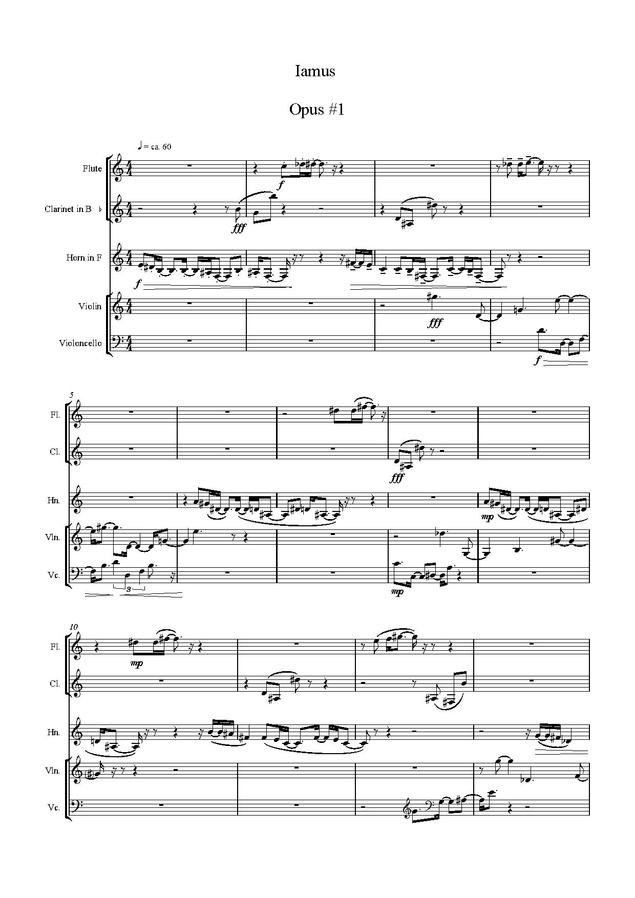
\includegraphics[width=0.4\linewidth]{rys01/lamus_notes.jpg}
    \caption{
      Zapis nutowy utworu \textit{Opus One},
      wygenerowany przez komputer \textit{Lamus}.
    }\label{fig:lamus_notes}
\end{figure}

Druga grupa algorytmów, generująca pliki audio, bazuje na klasie algorytmów
wywodzących się ze \textit{Stable Diffusion}~\cite{stablediffusion}.
Modele generujące pliki audio zgodne z opisem tekstowym 
(przykładowo \texttt{,,smutny jazz''} bądź \texttt{,,muzyka taneczna w stylu Depeche Mode''})
szkolone są w taki sam sposób jak algorytmy \textit{stable diffusion},
dane treningowe składają się z obrazów spektrogramów~\cite{riffusion}. 
Po trenowaniu, model jest wstanie wygenerować spektrogram zawierający
utwór muzyczny zgodny z poleceniem użytkownika (\ref{fig:riffusion_spectro}).
Wygenerowany przez model spektrogram jest konwertowany 
do sygnału dżwiękowego za pomocą odwrotnej transformaty Fouriera.

\begin{figure}[H]
    \centering
    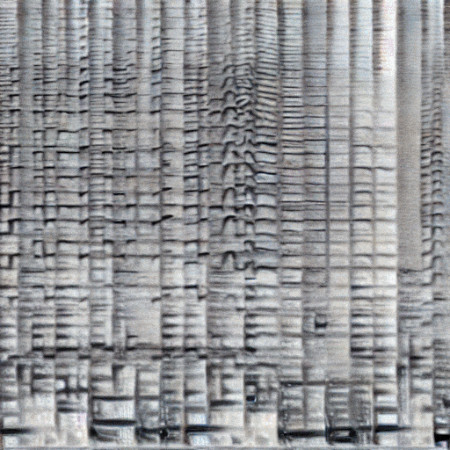
\includegraphics[width=0.4\linewidth]{rys01/riffusion_spectro.jpg}
    \caption{
      Przykładowy spektrogram wygenerowany przez algorytm \textit{Stable Riffusion}
      dla danych wejściowych \texttt{funk bassline with a jazzy saxophone solo}.
    }\label{fig:riffusion_spectro}
\end{figure}

Trzecia grupa algorytmów, symulowanie brzemienia instrumentów muzycznych, najczęściej wykorzystuje sieci
neuronowe trenowane na brzmieniu prawdziwych instrumentów~\cite{engel2017neural}~\cite{engel2020ddsp}. 
Tego typu algorytmy pozwalają symulowanie instrumentów o złożonych barwach, takich jak instrumenty
smyczkowe lub dęte oraz na płynne przechodzenie między brzmieniami różnych instrumentów muzycznych.

% TODO: check later
% https://github.com/Kinyugo/msanii

Metody opisane w rozdziale~\ref{traditional_algos} można porównać pod względem ich przydatności
dla użytkownika końcowego, czyli osoby zajmującej się produkcją nagrań muzycznych. Metoda pierwsza, 
generowanie zapisu symbolicznego, może wydawać się mniej zaawansowana niż generowanie całych plików dźwiękowych.
Jednakże, z perspektywy użytkownika, zapis symboliczny jest bardziej praktyczny,
ponieważ możliwe jest zaimportowanie go do programu DAW i późniejsza modyfikacja zapisu nutowego.
Obecnie dostępne modele generujące pełne nagrania z muzyką nie umożliwiają
szczegółowego edytowania parametrów wygenerowanego dźwięku, ponieważ operują bardzo wysokopoziomowo 
-- syntezują muzykę na podstawie opisu słownego. Podobne problemy występują również podczas wykorzystywania
algorytmów z grupy trzeciej, głębokie sieci neuronowe nie są przystosowane do ręcznej modyfikacji przez użytkownika.

Podsumowując, wykorzystanie wygenerowanego przez komputer zapisu nutowego jest proste,
ze względu na symboliczną naturę zapisu.
Wykorzystanie wygenerowanego przez komputer dźwięku jest ograniczone ze względu na fakt,
że do generowania złożonych sygnałów dźwiękowych wykorzystywane są techniki takie jak
głębokie sieci neuronowe, w których utrudniona jest dokładna kontrola nad konkretnymi
parametrami funkcjonowania sieci.

Niniejsza praca sugeruje nową metodę podejścia do problemu generowania sygnałów dźwiękowych,
którego nie da się zaklasyfikować do żadnej z wyżej wymienionych~(\ref{traditional_algos}) dziedzin komputerowej kompozycji muzycznej.
Graf przetwarzania sygnałów wytworzony przez algorytm implementowany w ramach pracy magisterskiej jest przepisem na gotowy elektroniczny instrument muzyczny,
który może być wykorzystany w programie do komponowania muzyki. Algorytm nie generuje bezpośrednio sygnału dźwiękowego, lecz tworzy
graf przetwarzania sygnałów, który jest zrozumiały dla użytkownika i pozwala na precyzyjne dostosowanie parametrów syntezy.
Tego typu proces generowania grafów przetwarzania sygnałów dźwiękowych może być porównany z procesem projektowania instrumentu muzycznego.

Modyfikowanie ścieżki przetwarzania sygnału jest techniką często wykorzystywaną w muzyce
elektronicznej, do tworzenia dźwięków o interesującej barwie bądź dynamice. Syntezatory dźwięku
dostępne na rynku często wyposażone są w tzw. \textit{patch bay}~(\ref{fig:mother32}), pozwalający na modyfikowanie
grafu przepływu sygnałów wewnątrz syntezatora, bądź połączenie go z zewnętrznym sprzętem muzycznym
bądź elektronicznym.

\begin{figure}[H]
    \centering
    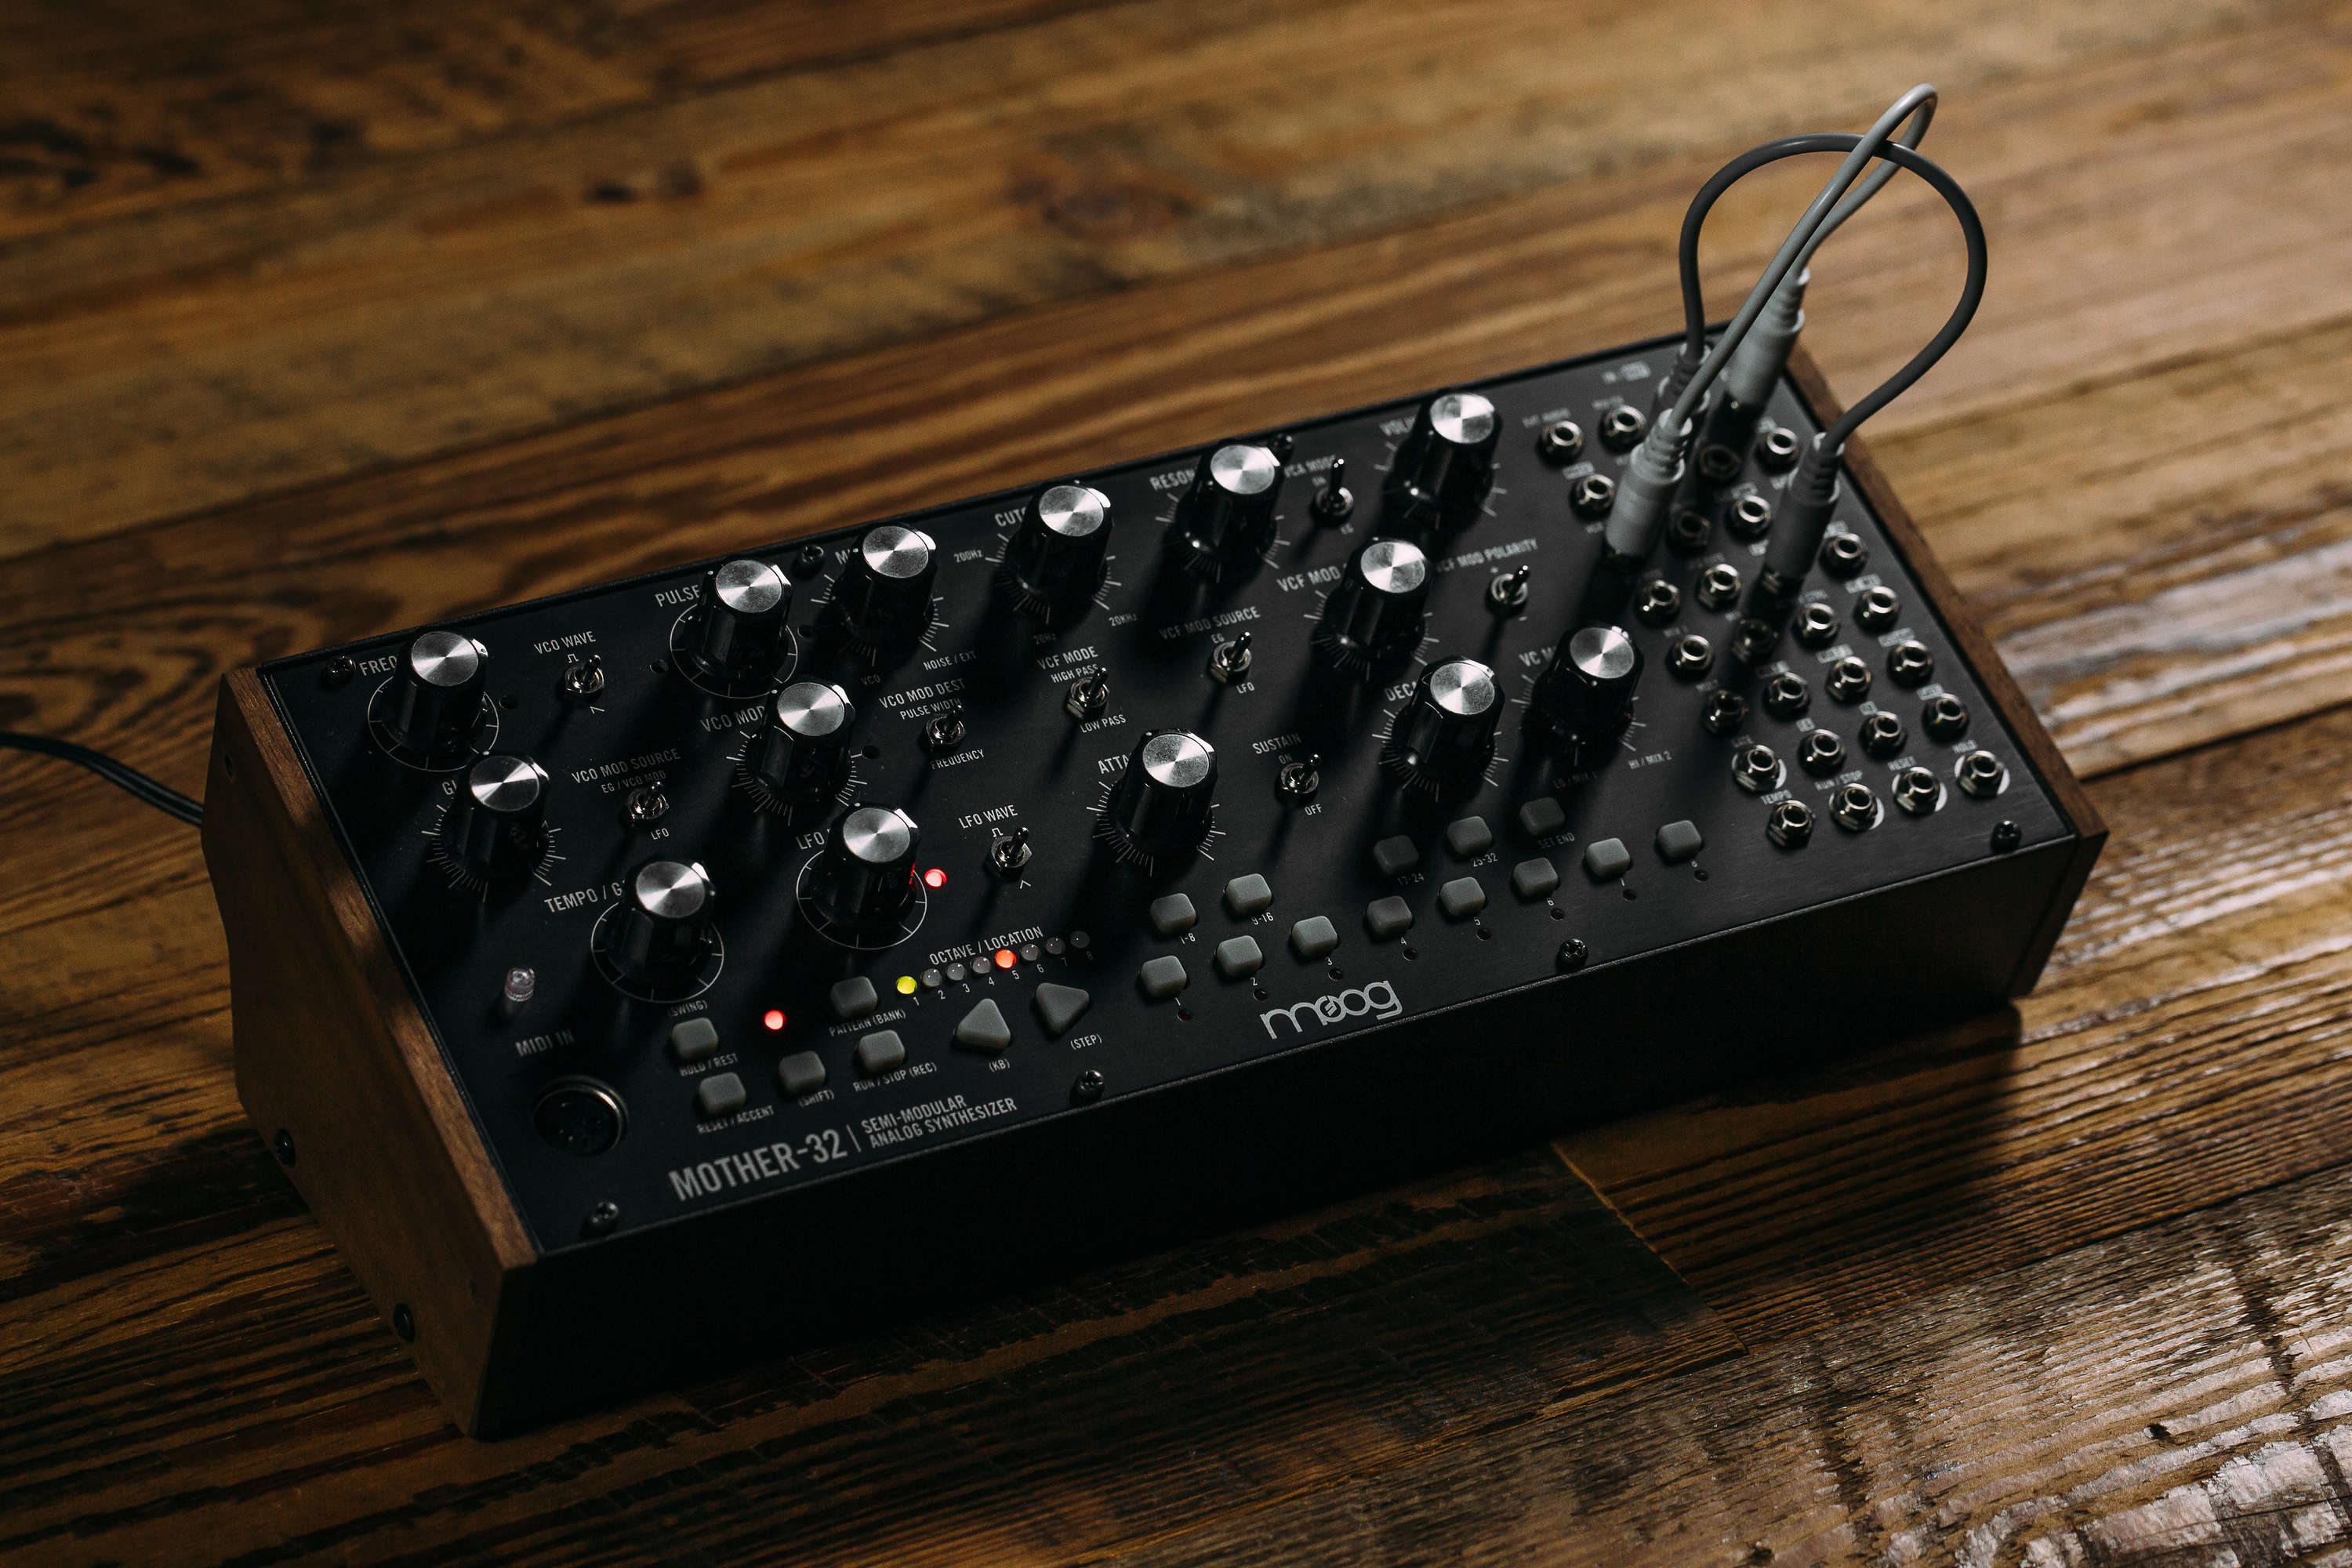
\includegraphics[width=0.7\linewidth]{rys01/mother32.jpg}
    \caption{
      Syntezator \textit{Mother 32} firmy \textit{Moog}, po prawej stronie widoczny
      jest \textit{patch bay} z podłączonymi przewodami, które nadpisują konfigurację
      połączeń między układami generującymi i przetwarzającymi sygnał dźwiękowy.
    }\label{fig:mother32}
\end{figure}


\section{Cel pracy}

Celem pracy jest \textbf{opracowanie algorytmu generacji grafów przetwarzania sygnałów, który
który wykona syntezę próbki dźwięku zadanej przez użytkownika}.
Problem poruszany w pracy można zakwalifikować do grupy zagadnień związanych
z pojęciami \textit{computer-aided design} oraz \textit{generative artificial intelligence}, zastosowanymi w dziedzienie inżynierii dźwięku. Docelowo
zaimplementowany algorytm będzie automatyzował pracę inżyniera dźwięku,
tworząc i konfigurując grafy przetwarzania sygnałów dźwiękowych, dostępne w
programach typu \textit{digital audio workstation}~(\ref{fig:ableton_patch}). Badania obejmują dwa zagadnienia:
\textbf{
\begin{enumerate}\label{research_types}
    \item opracowanie metody generowania grafu przetwarzania sygnałów oraz późniejszej modyfikacji grafu -- jego struktury i parametrów,
    \item dobór funkcji celu, na podstawie której algorytm optymalizujący będzie modyfikował graf przetwarzania sygnałów.
    \item przeprowadzenie badań symulacyjnych, które zweryfikują skuteczność opracowanego algorytmu.
    \item porównanie wyników badań symulacyjnych z pracami naukowymi o podobnej tematyce.
\end{enumerate}
}

\begin{figure}[H]
    \centering
    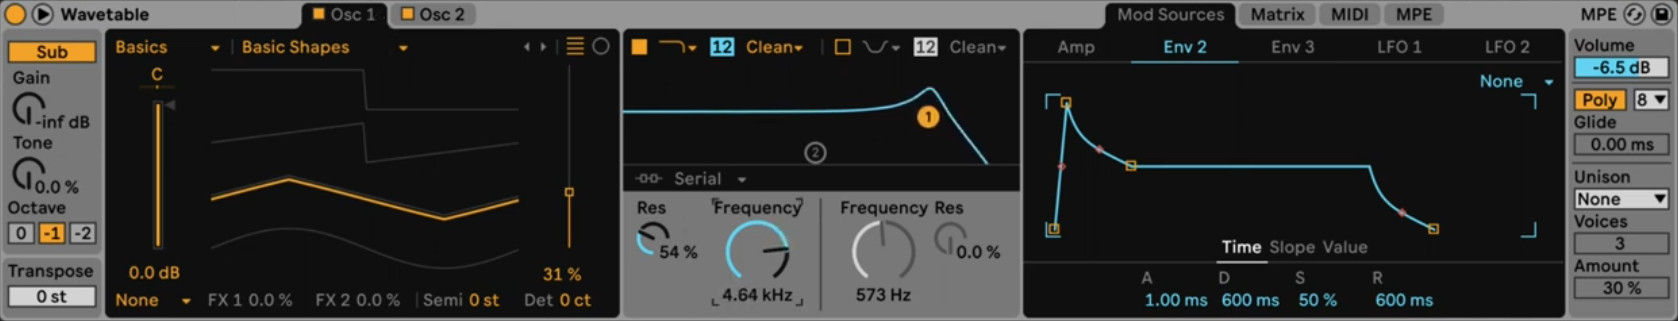
\includegraphics[width=0.8\linewidth]{rys01/ableton_patch.jpg}
    \caption{
      Zbiór parametrów konfigurujących syntezator dźwięku \textit{Wavetable} w programie \textit{Ableton}
    }\label{fig:ableton_patch}
\end{figure}

\subsection{Podstawy syntezy dźwięku}\label{sec:basics_of_sound_synthesis}

W syntezie dźwięku wykorzystuje się algorytmy generujące
i przetwarzające sygnały w zakresie częstotliwości słyszalnych.
Praca wykorzystuje powszechnie używane typy algorytmów syntezy,
opisane w~\cite{computational_music_synthesis}.

\subsubsection{Synteza FM}

Synteza FM wykorzystuje sygnał sinusoidalny jako źródło sygnału podstawowego
(\textit{carrier}). Zróżnicowane barwy dźwięku uzyskiwane są przez modulowanie
częstotliwości sinusoidy podstawowej przez inne sygnały sinusoidalne (\textit{modulators}),
które zazwyczaj generują sygnał o częstotliwości będącej wielokrotnością
częstotliwości podstawowej~\cite{spectral_audio_processing}. Siła modulacji
może być zmieniana w trakcie syntezy, co powoduje zmiany
w odczuwanej barwie dźwięku.

\subsubsection{Synteza subtraktywna}

W syntezie subtraktywnej wykorzystuje się sygnały dźwiękowe o dużej liczbie
składowych harmonicznych, takie jak sygnał piłokształtny lub kwadratowy.
Podstawową barwę dźwięku uzyskuje się przez dobór kilku sygnałów
o różnych kształtach, następnie sygnał jest filtrowany za pomocą filtrów
dolno-, górno- i pasmoprzepusowych~\cite{digital_filters}, aby
usunąć wybrane przez użytkownika składowe częstotliwościowe.
Dynamiczne zmiany w barwie dźwięku uzyskuje się poprzez modulowanie
częstotliwości odcięcia filtru.

\subsubsection{Algorytmy \textit{physical modeling}}

Algorytmy typu \textit{physical modeling} wykorzystują uproszczone
modele fizyczne rzeczywistych obiektów wytwarzających sygnały dźwiękowe,
takie jak struny czy membrany~\cite{lisp_synthesis}.


\subsubsection{symulacja efektu pogłosu/echa~\cite{reverb}~\cite{freeverb}}

Sygnał wygenerowany przez dany algorytm syntezy (lub połączenie wielu algorytmów)
może być przetworzony przez algorytmy symulujące echo lub pogłos (\textit{reverb, delay}).
Tego typu algorytmy naśladują roznoszenie się dźwięku w pudle rezonansowym
instrumentu bądź w dużej przestrzeni (sala koncertowa, jaskinia).
 

\subsection{Generowanie grafu przetwarzania sygnałów}

Proces syntezy dźwięku często jest przedstawiany jako graf przetwarzania sygnałów, w którym
każdy węzeł wykonuje na sygnale określoną operację.
Przykładowy graf przetwarzania sygnału dla syntezatora analogowego subtraktywnego
przedstawiony jest na schemacie~\ref{fig:minilogue_diagram}.
Pierwsze zagadnienie poruszane w pracy sprowadza się do opracowania algorytmu pozwalającego na wygenerowanie
grafu przetwarzania sygnałów DSP oraz jego późniejszą modyfikację. Przykładem modyfikacji grafu
może być wprowadzanie do niego nowych źródeł modulacji bądź zmiana algorytmu generującego sygnał.

\begin{figure}[H]
    \centering
    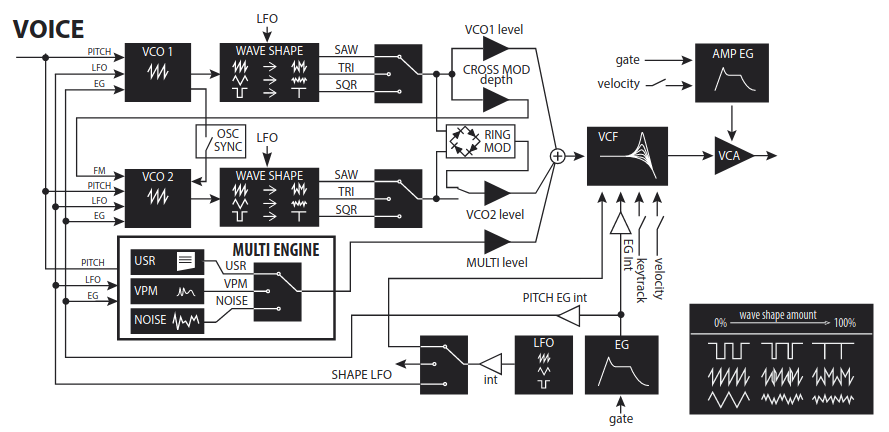
\includegraphics[width=0.8\linewidth]{rys01/minilogue_voice_block_diagram.png}
    \caption{
      Diagram blokowy pojedynczego głosu w syntezatorze 
      \textit{Minilogue xd} firmy \textit{Korg}~\cite{minilogue_diagram}.
    }\label{fig:minilogue_diagram}
\end{figure}

\subsection{Funkcja celu oceniająca podobieństwo barwy dźwieku}

Drugie zagadnienie obejmuje przetestowanie szeregu algorytmów, które można
wykorzystać do zbudowania funkcji celu, która będzie optymalizowana
poprzez~,,dostrajanie'' parametrów i struktury grafu przetwarzania sygnałów dźwiękowych.
Problem porównywania barwy dwóch sygnałów dźwiękowych nie jest problemem trywialnym,
ponieważ wymaga zamodelowania wrażeń psychoakustycznych~\cite{engel2020ddsp} odczuwanych
podczas odsługu próbki dźwięku.
Skuteczność danej funkcji celu finalnie musi być poddana subiektywnej ocenie,
ponieważ nie istnieją obiektywne metryki mierzące z natury subiektywne odczucia słuchacza.
Praca proponuje wykorzystanie współczynników cepstralnych sygnału (MFCC) w połączeniu
z dynamicznym skalowaniem czasu (\textit{dynamic time wrapping}, DTW) jako funkcji celu.
Proces wyboru funkcji celu został
opisany w rozdziale~\ref{target_function_chapter}.

\subsection{Problem optymalizacyjny}

W pracy rozwiązywany jest problem optymalizacyjny, w którym
struktura oraz parametry grafu przetwarzania sygnałów dostosowywane
są tak, aby wygenerować zadaną próbkę dźwięku. Tak wytworzony
graf może być wykorzystany jako elektroniczny instrument muzyczny. 

% Następnie, dla danego układu $N$ węzłów przetwarzania oraz dla macierzy połączeń $C$, 
% należy rozwiązać następujący problem optymalizacji, należy rozwiązać problem
% maksymalizacji funkcji opisanej równaniem~\ref{eq:target_function} dla
% parametrów wszystkich wejść $i_j$ oraz $o_j$, które nie są połączone bezpośrednio
% pomiędzy węzłami.




\section{Zakres pracy, plan badań}\label{chap:thesis_scope}

\subsection{Metody generowania grafu przetwarzania sygnałów oraz późniejsza modyfikacja grafu}

Głównym problemem przy generowaniu grafu przetwarzania sygnałów są ograniczenia nałożone na strukturę grafu,
które należy spełnić, by graf był logicznie interpretowalny jako łańcuch przetwarzania sygnałów.
Graf musi być grafem skierowanym, który nie zawiera pętli o dodatnim sprzężeniu zwrotnym.
% Struktura grafu powinna być możliwie jak najbardziej przejrzysta dla użytkownika. 
Automatyczna ewolucja może dążyć w kierunku wykorzystania nadmiarowej liczby
bloków przetwarzania sygnału, jeśli funkcja celu nie będzie zawierała kary za zbyt złożone grafy.
Podobne prace~\cite{evolutionary_puredata} wykorzystują podejście oparte o 
\textit{mixed-typed carthesian genetic programming}, które będzie punktem startowym dla pracy.
Finalnie, badania dążą do wyznaczenia algorytmu o następujący właściwościach:

\begin{enumerate}
    \item algorytm generuje grafy będące logicznie spójnymi łańcuchami przetwarzania dźwięku (skierowany, bez pętli o dodatnim sprzężeniu zwrotnym w natężeniu sygnału),
    \item algorytm maksymalizuje wykorzystanie poszczególnych bloków przetwarzania w grafie, co minimalizuje finalny rozmiar grafu, czyniąc go bardziej czytelnym,
    \item generowany graf posiada reprezentację umożliwiającą wykonanie krzyżowania dwóch grafów przetwarzania sygnału. Graf będący wynikiem krzyżowania nadal musi być poprawnym grafem przetwarzania sygnału.
\end{enumerate}

\noindent
Elementami grafu przetwarzania sygnałów są używane powszechnie w syntezie dźwięku algorytmy,
opisane w sekcji~\ref{sec:basics_of_sound_synthesis}.

\subsection{Dobór funkcji błędu: różnica między wygenerowanym a docelowym sygnałem dźwiękowym}

Funkcja celu poszukiwana w ramach projektu musi określać, jak dobrze sygnał wygenerowany przez
graf przetwarzania sygnałów pokrywa się z sygnałem docelowym. Porówanie sygnałów musi skupiać się
na cechach sygnału, które są najbardziej słyszalne dla ludzkiego ucha. Jednocześnie funkcja nie powinna
,,karać'' sygnałów, które są względem siebie przesunięte w fazie. Wśród algorytmów, które zostały wybrane
do przetestowania w ramach projektów zawarte są:

\begin{enumerate}
  \item algorytmy porównywania sygnałów oparte o transformatę Fouriera~\cite{sliding_fourier}~\cite{mfcc},
  \item techniki wykorzystywane do generowania~,,cyfrowych podpisów'' sygnałów dźwiękowych (\textit{sound fingerprinting})~\cite{computer_vision_music_identification},
  \item algorytmy wykrywające spadek jakości dźwięku z perspektywy psychoakustycznej~\cite{peaq}~\cite{frechet_audio_distance}.
\end{enumerate}

\section{Struktura i zawartość pracy}

% Praca podzielona jest na następujące części:

Rozdział \textbf{Definicja problemu} formalizuje i opisuje problem optymalizacyjny rozwiązywany w pracy.
W rozdziale \textbf{Analiza i wybór funkcji celu} opisano proces porównywania funkcji z dziedziny przetwarzania sygnałów,
które pozwalają określić jak podobna jest barwa dźwięku dwóch sygnałów dźwiękowych i
uzasadniono wybór funkcji celu, która została zastosowana w pracy.
Rozdział \textbf{Algorytm rozwiązania} opisuje algorytm wykorzystany do rozwiązania problemu
zdefiniowanego w rozdziale~\ref{chap:problem_definition}.
W rozdziale \textbf{Implementacja grafu przetwarzania sygnałów} opisane zostało zaimplementowane w ramach pracy środowisko eksperymentalne,
pozwalające na wytwarzanie grafów przetwarzania sygnałów o dowolnej strukturze.
Przedstawione są w nim również zaimplementowane algorytmy syntezy i przetwarzania sygnałów dźwiękowych.
Rozdział \textbf{Badania symulacyjne} opisuje proces badawczy, w którym narzędzia wytworzone w
rozdziałach~\ref{dsp_graph_chapter} oraz~\ref{target_function_chapter}
zostały wykorzystane do automatycznego wytworzenia grafu DSP, który naśladuje barwę zadanej próbki dźwięku.
Porównuje uzyskane wyniki z podobną pracą badawczą~\cite{evolutionary_puredata}.
Rozdział \textbf{Analiza wyników, możliwe drogi dalszego rozwoju} podsumowuje uzyskane wyniki badań, podejmuje dyskusję nad ogólną skutecznością i przydatnością zaimplementowanego rozwiązania oraz
kreśli potencjalne drogi dalszego rozwoju prac badawczych w podobnej tematyce. W czasie, gdy niniejsza praca była tworzona, zostały opublikowane badania
dotyczące podobnego problemu~\cite{ieee_synth_programming}, rozdział podejmuje dyskusję o różnicach w podejściu do problemu oraz potencjalnych
zalet i wad każdego z podejść. \textbf{Dodatek A} zawiera instrukcję wdrożeniową dla
zaimplementowanego w ramach pracy środowiska eksperymentalnego, w \textbf{Dodatku B}
opisana jest zawartość załączonej do pracy płyty DVD\@.


\chapter{Graf przetwarzania sygnałów} \label{dsp_graph_chapter}

Na potrzeby badań zostało zaimplementowane środowisko, pozwalające na dynamiczne tworzenie grafów przetwarzania
sygnałów~(\ref{fig:example_simple_analog_synth}). W projekcie nie zostało zastosowane gotowe rozwiązanie symulujące syntezator modułowy, takie jak
\href{https://www.bespokesynth.com/}{Bespoke Synth}~\cite{bespoke}, \href{https://vcvrack.com/Rack}{VCVRack}~\cite{vcvrack}
lub \href{https://puredata.info/}{Pure Data}~\cite{pure_data}, ponieważ
nie udostępniały one gotowego interfejsu pozwalającego na łatwą integrację z językiem \texttt{Python}.
Istniejące w internecie gotowe przykłady algorytmów syntezy audio pozwoliły na szybkie zaimplementowanie
środowiska eksperymentowego, które posiada szeroki zbiór dostępnych algorytmów DSP oraz w przystępny sposób
interfejsuje się z językiem \texttt{Python}, co umożliwia wykorzystanie gotowych pakietów obliczeniowych z dziedziny przetwarzania sygnałów.

\begin{figure}[H]
    \centering
    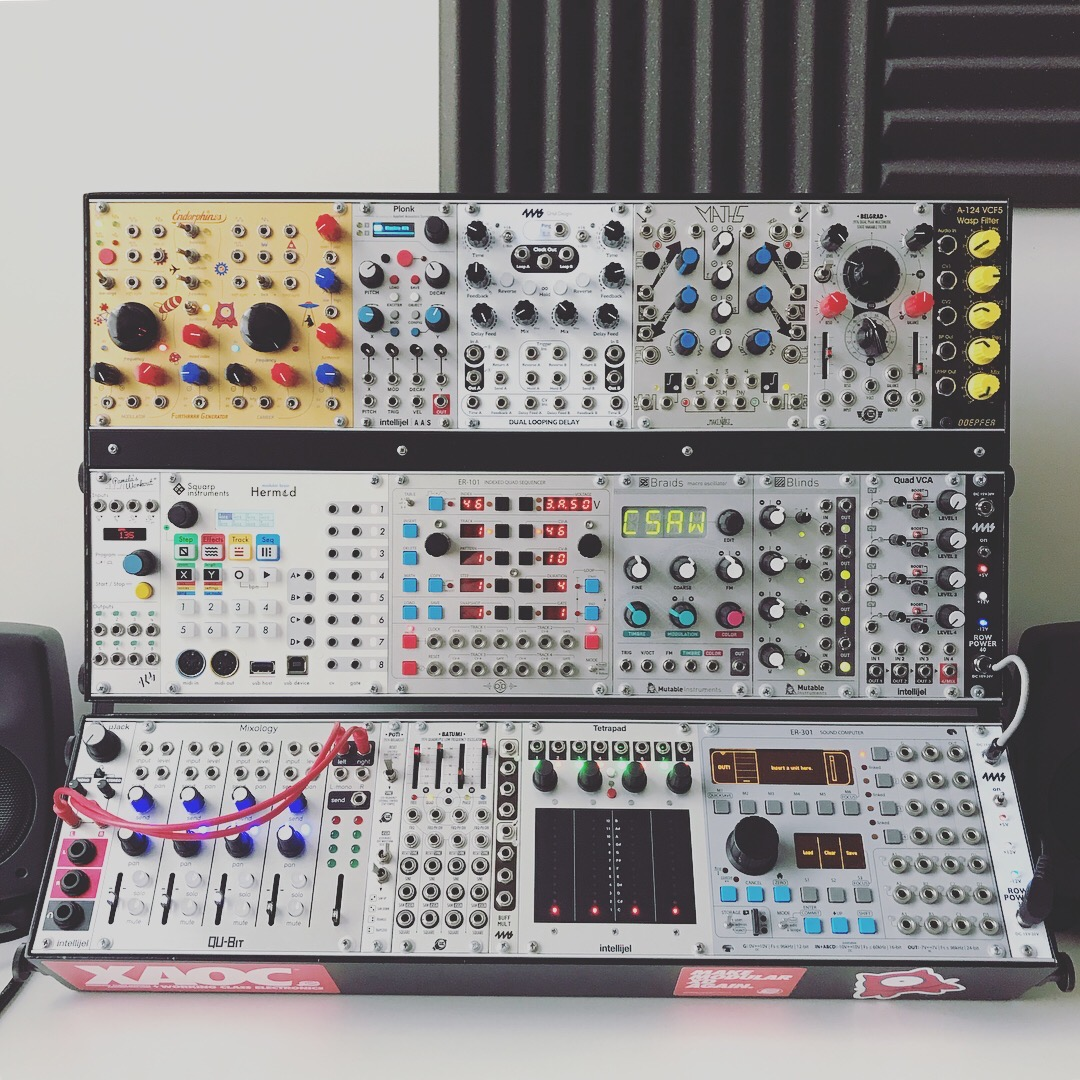
\includegraphics[width=0.4\linewidth]{rys02/eurorack.jpg}
    \caption{
      Przykładowy układ modułów w standardzie \textit{Eurorack}~\cite{eurorack}.
      W prawym dolnym rogu widoczne połączenia modulujące między modułami.
    }
    \label{fig:eurorack_setup}
\end{figure}

\section{Podstawy syntezy dźwięku w syntezatorach modułowych}

Proces syntezy dźwięku może zostać przedstawiony jako zbiór węzłów wykonujących syntezę lub
przetwarzanie sygnału audio oraz połączeń między węzłami. Przykładowe elementy grafu:

\begin{enumerate}
  \item Węzły:
    \begin{enumerate}
      \item generujące sygnał:
        \begin{itemize}
          \item synteza sygnałów (sinusoida, trójkąt, sygnał prostokątny),
          \item sygnał modulujący (LFO, ADSR).
        \end{itemize}
      \item przetwarzające sygnał:
        \begin{itemize}
          \item filtry (górnoprzepustowy, dolnoprzepustowy, pasmowo-przepustowy),
          \item efekty (pogłos, echo).
        \end{itemize}
    \end{enumerate}
  \item Połączenia między węzłami:
    \begin{itemize}
      \item modulowanie parametrów syntezy i przetwarzania sygnału.
    \end{itemize}
\end{enumerate}

\noindent
Odpowiednikiem implementowanego środowiska w świecie rzeczywistym są syntezatory modułowe (przykładowo~\ref{fig:eurorack_setup}),
które pozwalają na dowolne łączenie modułów wykonujących operacje DSP.
Barwę dźwięku w syntezatorze modyfikuje się na dwa sposoby:
\begin{enumerate}
  \item Ustawienie stałej wartości danego parametru w węźle DSP,
  \item Modulacja wartości danego parametru w węźle DSP za pomocą wartości wyjściowej innego węzła.
\end{enumerate}

\begin{figure}[H]
    \centering
    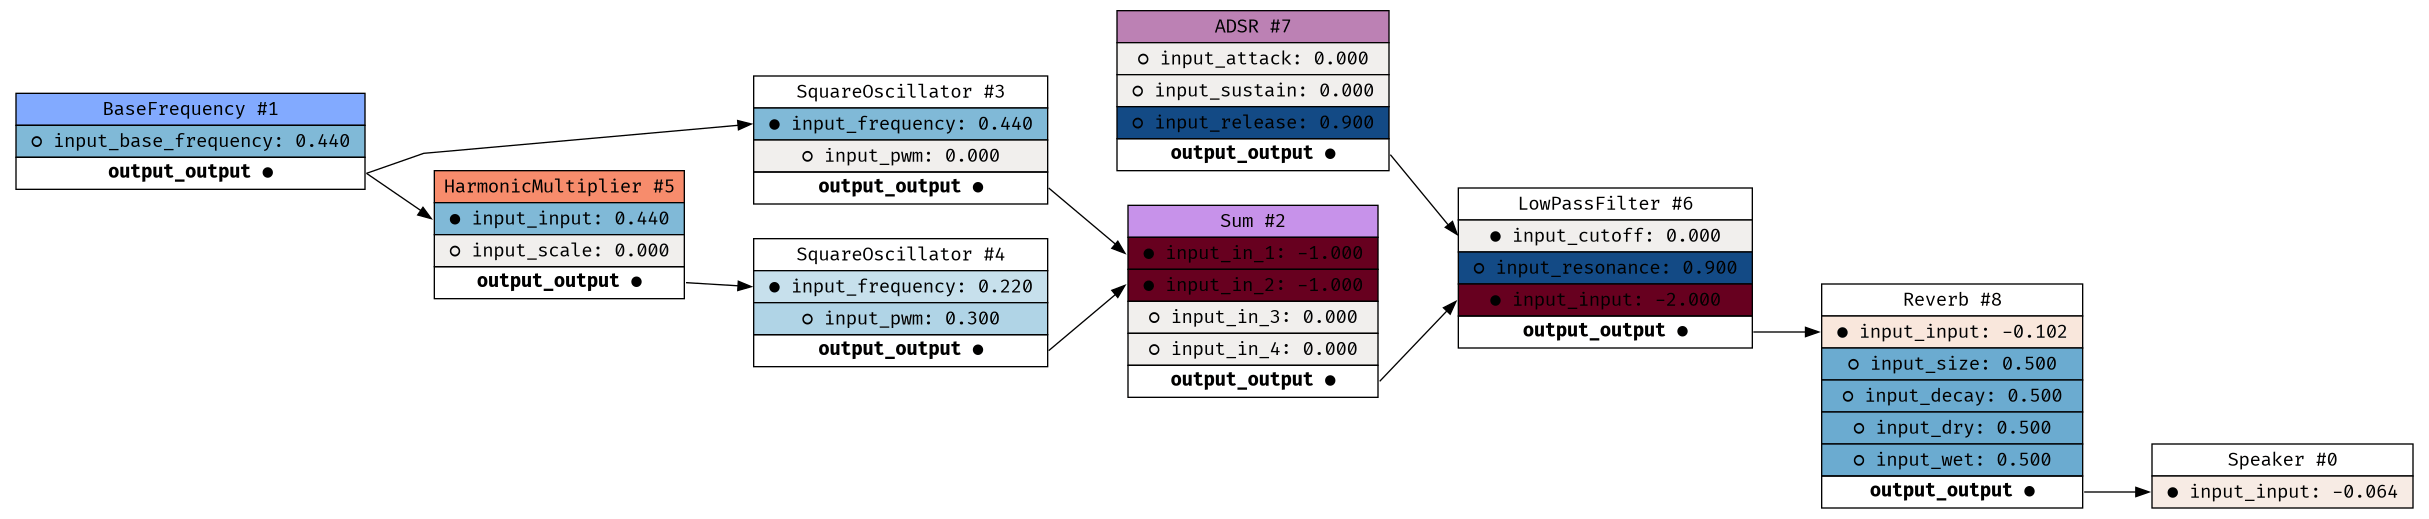
\includegraphics[width=0.9\linewidth]{rys02/luthier_simple_analog.png}
    \caption{
      Przykładowy układ węzłów DSP w zaimplementowanym środowisku eksperymentowym.
      Układ wykonuje syntezę subtraktywną z modulowaną wartością częstotliwości granicznej filtru niskoprzepustowego
      oraz dodaje efekt pogłosu (\textit{reverb})~\cite{reverb}.
    }
    \label{fig:example_simple_analog_synth}
\end{figure}

\noindent
Dla przykładowego układu DSP, przedstawionego na rysunku~\ref{fig:example_simple_analog_synth},
skonfigurowane są między innymi parametry:

\begin{enumerate}
  \item Częstotliwość podstawowa (węzeł \texttt{BaseFrequency \#1}),
  \item wartość, przez którą mnożona jest częstotliwość podstawowa w węźle \texttt{HarmonicMultiplier \#5},
  \item Wartości \texttt{input\_pwm} w węzłach \texttt{SquareOscillator} \texttt{\#3} oraz \texttt{\#4},
  \item Parametry algorytmu pogłosu w węźle \texttt{Reverb \#8}.
\end{enumerate}

\noindent
Z kolei wartość parametru \texttt{input\_cutoff} w węźle \texttt{LowPassFilter \#6} \textbf{jest modulowana}
przez sygnał wychodzący w węźle \texttt{ADSR \#7}, co pozwala na dynamiczne zmiany
częstotliwości odcięcia filtru w czasie, wzbogacając barwę generowanego dźwięku.

\section{Wymagania} \label{sec:requirements}

W ramach pracy zostały zdefiniowane wymagania dotyczące implementowanego później środowiska eksperymentowego,
opisane w niniejszym rozdziale.

\subsection{Węzły DSP}

Pojedynczy węzeł DSP może zostać opisany za pomocą trzech cech:

\begin{enumerate}
  \item Zbiór sygnałów wejściowych,
  \item zbiór sygnałów wyjściowych,
  \item wykonywana przez węzeł operacja.
\end{enumerate}


% \begin{multicols}{2}
\begin{figure}[H]
    \centering
    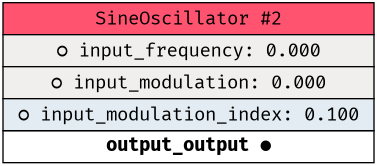
\includegraphics[width=0.4\linewidth]{rys02/example_sine_node.png}
    \caption{
      Węzeł DSP w zaimplementowanym środowisku eksperymentowym, generujący falę sinusoidalną z możliwością modulacji fazy.
    }
    \label{fig:example_sine_node}
\end{figure}

\begin{figure}[H]
    \centering
    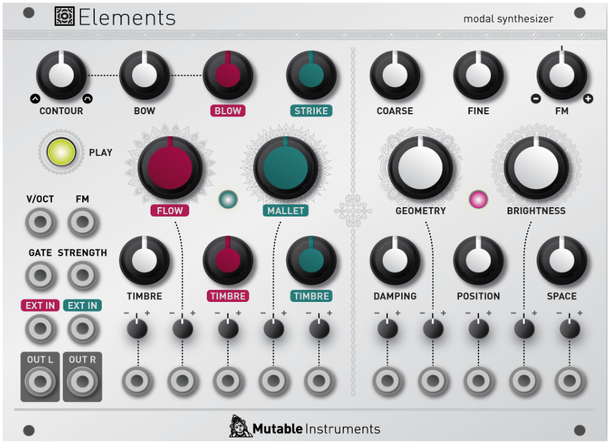
\includegraphics[width=0.45\linewidth]{rys02/mutable_instruments_elements.png}
    \caption{
      Moduł syntezy \textit{Mutable Instruments Elements}, umożliwiający ręczne ustawianie \textbf{oraz} modulację
      parametrów. Moduł wykonuję syntezę typu \textit{physical modeling} \cite{lisp_synthesis}.
    }
    \label{fig:example_eurorack_module}
\end{figure}
% \end{multicols}

\noindent
Przykładowo, przedstawiony na rysunku~\ref{fig:example_sine_node} węzeł posiada:
\begin{enumerate}
  \item sygnały wejściowe:
  \begin{itemize}
    \item \texttt{input\_frequency} - częstotliwość generowanej sinusoidy,
    \item \texttt{input\_modulation} - wartość modulacji fazy, według równania~\ref{eq:fm_sine},
    \item \texttt{input\_modulation\_index}.
  \end{itemize}
  \item Sygnały wyjściowe:
  \begin{itemize}
    \item \texttt{output\_output} - wartość generowanego sygnału sinusoidalnego.
  \end{itemize}
\end{enumerate}

\noindent
Węzeł generuje sygnał sinusoidalny o fazie modulowanej poprzez parametr \texttt{input\_modulation} z siłą modulacji ustawianą przez
parametr \texttt{input\_modulation\_index}, opisane za pomocą równania~\ref{eq:fm_sine}
(jest to uproszczenie równania syntezy FM przedstawionego w \cite{spectral_audio_processing}) oraz listingu~\ref{lst:sine_fm}:

\begin{equation} \label{eq:fm_sine}
  f(t) = sin(t * f + m * m_i)
\end{equation}

\begin{lstlisting}[language=Rust, caption=Implementacja węzła SineOscillator.,label={lst:sine_fm}]
impl DspNode for SineOscillator {
    fn tick(&mut self) {
        let frequency = (self.input_frequency * 1000.0).abs();
        let phase_diff = (2.0 * std::f64::consts::PI * frequency) / SAMPLE_RATE;
        self.output_output =
            (self.phase + self.input_modulation * self.input_modulation_index * 10.0).sin();
        self.phase += phase_diff;

        while self.phase > std::f64::consts::PI * 2.0 {
            self.phase -= std::f64::consts::PI * 2.0
        }
    }
}
\end{lstlisting}

\noindent
\textbf{Wymaganie:} zaimplementowane w ramach pracy środowisko eksperymentalne musi pozwalać na zdefiniowanie węzłów DSP, które generują lub
przetwarzają sygnał. Węzły posiadają sloty wejściowe, z których czytają wartości parametrów sterujących wykonywanymi 
przez węzły operacjami.

\subsection{Połączenia między węzłami -- modulacja parametrów węzłów} \label{sec:modulation_requirements}

Każdy węzeł DSP w środowisku eksperymentowym posiada zbiór parametrów wejściowych. Poza możliwością
ustawienia danego parametru wejściowego na konkretną wartość, możliwa jest też modulacja parametru
wejściowego. Na rysunku~\ref{fig:fm_mod_example} przedstawiony jest przykładowy układ węzłów i modulacji,
które pozwalają na uzyskanie syntezy FM.

\begin{figure}[H]
    \centering
    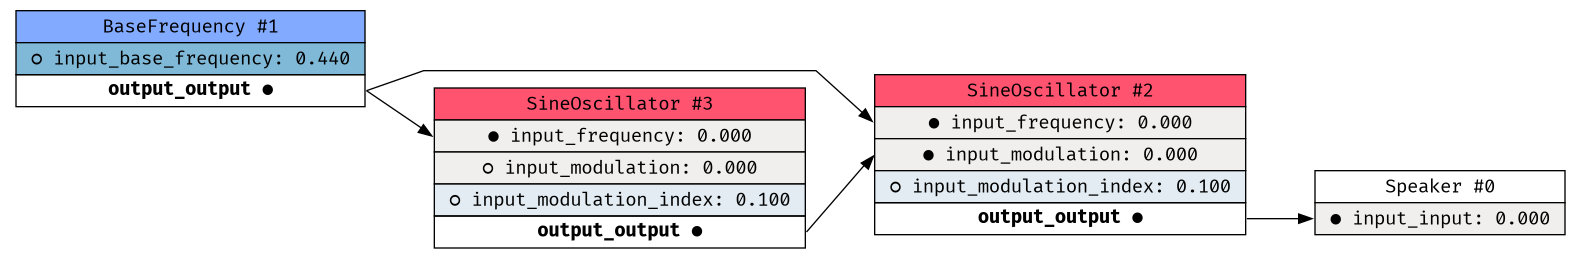
\includegraphics[width=1.0\linewidth]{rys02/fm_mod_example.png}
    \caption{
      Przykładowa modulacja parametru \texttt{input\_modulation} za pomocy sygnału sinusoidalnego, charakterystyczna dla syntezy typu FM \cite{computational_music_synthesis}.
    }
    \label{fig:fm_mod_example}
\end{figure}

\begin{multicols}{2}
\begin{figure}[H]
    \centering
    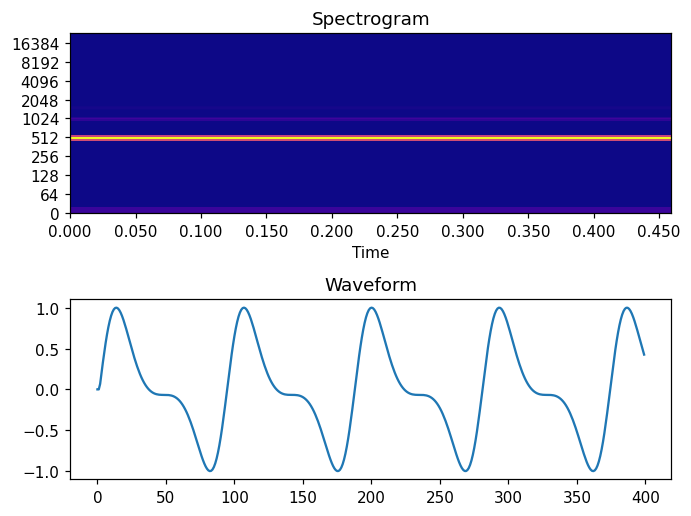
\includegraphics[width=1.0\linewidth]{rys02/spectro_fm.png}
    \caption{
      Spektrogram oraz wykres sygnału wygenerowanego za pomocą układ z rysunku~\ref{fig:fm_mod_example}.
      Widoczne dodatkowe składowe harmoniczne wpływające na barwę dźwięku.
    }
    \label{fig:fm_mod_spectra}
\end{figure}

\begin{figure}[H]
    \centering
    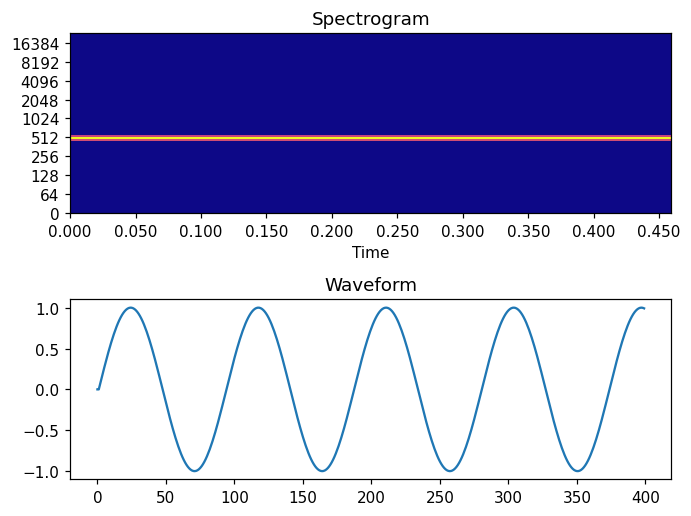
\includegraphics[width=1.0\linewidth]{rys02/spectro_no_fm.png}
    \caption{
      Spektrogram oraz wykres sygnału wygenerowanego przez układ z rysunku~\ref{fig:fm_mod_example}
      \textbf{po usunięciu} połączenia modulującego fazę oscylatora \texttt{\#2}.
      Widoczna tylko jedna składowa harmoniczna: częstotliwość podstawowa.
    }
    \label{fig:fm_no_mod_spectra}
\end{figure}
\end{multicols}

\noindent
\textbf{Wymaganie:} zaimplementowane środowisko pozwala na modulowanie
dowolnego parametu wejściowego w węźle za pomocą wartości wyjściowej dowolnego węzła,
\textbf{w tym modulowanie wejścia węzła wyjściem tego samego węzła} (tzw. \textit{circular patching},
popularny zarówno w syntezie FM jak i w układach analogowych).

\subsection{Graf przetwarzania sygnałów}

Węzły DSP oraz połączenia między nimi istnieją w ramach danego grafu przetwarzania sygnałów, który agreguje
wiele węzłów i wiele połączeń. Instancja grafu DSP musi umożliwiać dynamiczną modyfikację grafu, na którą składają się następujące operacje:

\begin{enumerate}
  \item Dodanie nowego węzła,
  \item Dodanie nowego połączenia między węzłami,
  \item Usunięcie węzła,
  \item Usunięcie połączenia między węzłami,
  \item Ustawienie $i$-tego parametru wejściowego danego węzła na określoną przez użytkownika wartość.
\end{enumerate}

\noindent
Po utworzeniu grafu, użytkownik musi mieć możliwość ,,uruchomienia'' na grafie procesu syntezy dźwięku,
który zwróci użytkownikowi strukturę danych zawierającą wygenerowany sygnał. \\

\noindent
\textbf{Wymaganie:} zaimplementowane środowisko pozwala na dynamiczną modyfikację grafu przetwarzania sygnałów oraz na 
wygenerowanie sygnału z wytworzonego w środowisku grafu.


\subsection{Automatyzacja pracy ze środowiskiem eksperymentowym za pośrednictwem języka \texttt{Python}}

\textbf{Wymaganie:} ze względu na dużą dostępność gotowych algorytmów optymalizacyjnych oraz DSP w języku \texttt{Python}
(\cite{librosa}, \cite{2020SciPy-NMeth}), zaimplementowane środowisko musi udostępniać interfejs pozwalający
na wykonywanie operacji zdefiniowanych w wymaganiach za pośrednictwem języka \texttt{Python}.

\section{Opis zaimplementowanego środowiska eksperymentowego}

W ramach pracy zaimplementowane zostało środowisko pozwalające na dynamiczne budowanie grafów DSP oraz
na generowanie sygnałów dźwiękowych za pomocą wytworzonych grafów,
według wymagań opisanych w sekcji~\ref{section:requirements}. Środowisko zaimplementowano w języku \texttt{Rust},
dzięki czemu proces syntezy sygnałów jest szybszy niż w przypadku implementacji w języku interpretowanym.
Zaimplementowana biblioteka udostępnia interfejs zgodny ze standardem
\textit{Python Extension Module}~\cite{python_extension_module}.

\subsection{Przykłady użycia}

\subsubsection{Utworzenie grafu}

Zaimplementowane środowisko pozwala na tworzenie grafów przetwarzania sygnałów za pomocą poleceń w języku \texttt{Python}.
Listing~\ref{lst:simple_sine} przedstawia proces tworzenia prostego grafu generującego sygnał sinusoidalny.

\begin{lstlisting}[language=python, caption=Utworzenie prostego grafu generującego sygnał sinusoidalny., label={lst:simple_sine}]
g = DspGraph()

carrier = g.add_sine(SineOscillator())
g.patch(
  g.base_frequency_node_id, "output_output",
  carrier, "input_frequency"
)

g.patch(
  carrier, "output_output",
  g.speaker_node_id, "input_input"
)

display(Image(g.draw()))
\end{lstlisting}

\begin{figure}[H]
    \centering
    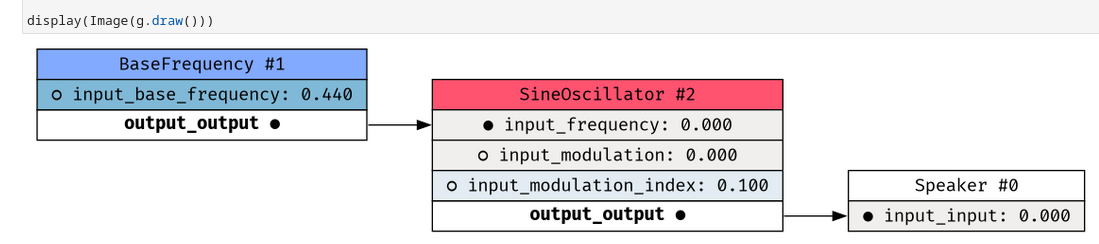
\includegraphics[width=1.0\linewidth]{rys02/simple_graph_creation_example.png}
    \caption{
      Wynik wykonania kodu przedstawionego w listingu~\ref{lst:simple_sine} w środowisku \textit{Jupyter Notebook},
      wizualizacja utworzonego grafu.
    }
    \label{fig:example_graph_creation_jupyter}
\end{figure}

\subsubsection{Uruchomienie procesu syntezy dźwięku}

Jak pokazano na listingu~\ref{lst:numpy_rust}, środowisko eksperymentalne zaimplementowane w ramach pracy w języku \texttt{Rust}
zwraca obiekty typu \texttt{ndarray}, wykorzystywane w większości pakietów obliczeniowych wykorzystywanych w języku \texttt{Python}.
Umożliwia to wykorzystanie gotowych bibliotek dostępnych w języku \texttt{Python},
aby przeanalizować sygnał lub zoptymalizować parametry syntezy \cite{2020SciPy-NMeth} \cite{librosa}.

\begin{lstlisting}[language=python, caption=Typ danych zwracanych przez środowisko eksperymentalne., label={lst:numpy_rust}]
>>> generated_signal = g.play(num_samples=100)
>>> type(generated_signal)
<class `numpy.ndarray'>
\end{lstlisting}

\subsection{Detale techniczne}

\subsubsection{Połączenia między węzłami w grafie}

Ponieważ wymagania zdefiniowane w rozdziale \ref{sec:requirements} zawierają dynamiczne modyfikowanie grafu przetwarzania sygnałów,
nie jest możliwe spredefiniowanie mechanizmu wymiany danych między połączonymi węzłami.
Podczas implementacji rozważane były następujące architektury:

\begin{enumerate}
  \item Przejście przez graf przed uruchomieniem syntezy i określenie kolejności wywołania węzłów,
  \item Wykorzystanie struktury danych kolejki w każdym połączeniu,
  \item Bezpośrednie przepisywanie wartości wyjść z węzłów do modulowanych przez nie wejść po każdej iteracji przetwarzania. \label{test}
\end{enumerate}

Ostatecznie wybrane zostało podejście 3, ze względu na konieczność spełnienia wymagania
\ref{sec:modulation_requirements}, konkretnie możliwości modulowania wejścia danego węzła
przez wyjście tego samego węzła, co uniemożliwia wykorzystanie podejścia 1. Jednocześnie
podejście 3 jest łatwiejsze do implementacji niż podejście 2. Implementację mechanizmu
przesyłu danych między węzłami ułatwiło wykorzystanie makr proceduralnych, opisane w sekcji \ref{sec:proc_macro}.

\subsubsection{Zastosowanie \textit{procedural macros} do automatycznej generacji akcesorów struktur węzłów} \label{sec:proc_macro}

% Przesyłanie wartości modulacji między węzłami grafu wymaga zdefiniowania struktur mapujących
% poszczególne pola struktur danych na ich indeksy, dzięki czemu możliwe jes
Podczas implementacji grafu DSP zostały wykorzystane makra proceduralne~\cite{proc_macro},
które umożliwiają automatyczne zaimplementowanie metod odczytujących $i$-te wejście
lub wyjście danego węzła. Alternatywnym podejściem byłoby wykorzystanie struktur takich
jak słowniki lub mapy, które umożliwiają na inspekcję kluczy w strukturze danych podczas
działania programu i dostęp do nich za pomocą indeksu, jednakże takie podejście zmniejsza
wydajność programu i nie wykorzystuje wykorzystywanie systemu typów wbudowanego w język,
co potencjalnie może być źródłem błędów podczas utrzymywania dużego zbioru węzłów i algorytmów,
które wykonują. Wykorzystanie makr proceduralnych pozwala na ograniczenie powtarzalnych
implementacji podobnych akcesorów i zachowanie zalet silnego systemu typów języka
\texttt{Rust}. % ponieważ na poziomie implementacji

\subsubsection{Implementacja natywnego modułu dla języka \texttt{Python}}

Aby umożliwić wykorzystanie grafu przetwarzania sygnałów z poziomu języka
Python, wykorzystano narzędzie \textit{Maturin}~\cite{maturin}, służące
do implementowania rozszerzeń zgodnych ze standardem \textit{Python Extension Module}~\cite{python_extension_module}
w języku \texttt{Rust}.


\chapter{Funkcja celu -- porównanie barwy dźwięku}~\label{target_function_chapter}

Aby stopniowo dostosować graf przetwarzania sygnałów tak, aby imitował zadaną próbkę dźwięku,
należy wykorzystać funkcję celu, która maleje wraz ze wzrostem podobieństwa
barwy dźwięku między próbki zadaną i sygnałem generowanym przez graf.

\begin{figure}[H]\label{fig:waveform_not_equal_to_perception}
    \centering
    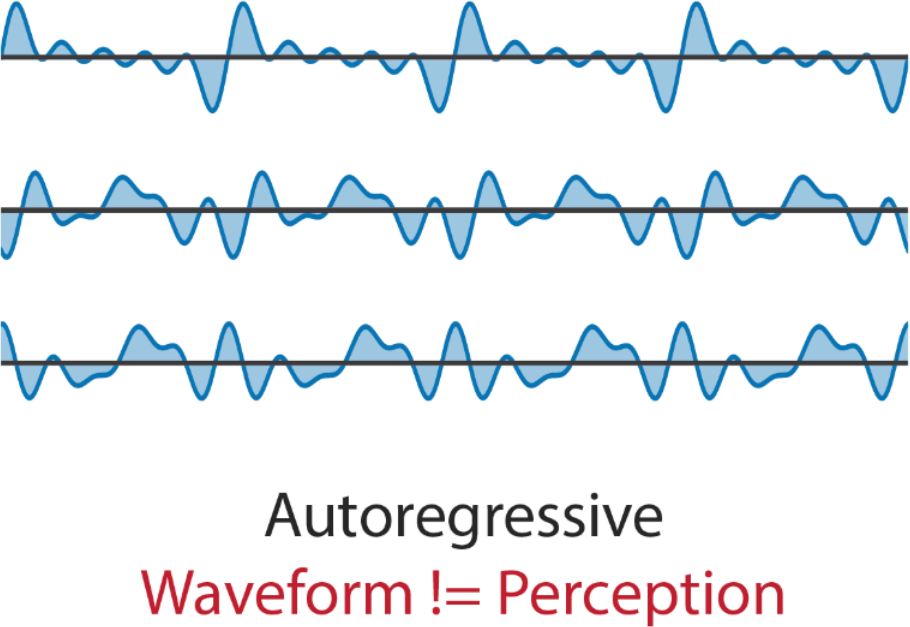
\includegraphics[width=0.45\linewidth]{rys03/d_dsp_example_graph.png}
    \caption{
      Przykład trzech próbek dźwięku, które dla słuchacza brzmią identycznie, mimo
      znacznych różnic w kształcie fali. Źródło obrazka:~\cite{engel2020ddsp}.
    }
\end{figure}

\section{Porównanie barwy dźwięku w literaturze}\label{sec:timbre_comparison_literature_overview}

Żadna z prac przeanalizowanych podczas przeglądu literatury
(\cite{engel2020ddsp},~\cite{ieee_synth_programming},~\cite{ddx7},~\cite{riffusion},~\cite{evolutionary_puredata},~\cite{parallel_evolutionary_optimization_synth_parameters},~\cite{mfcc_dtw})
nie wykorzystuje metod porównywania sygnału osadzonych jedynie w dziedzinie czasu, ponieważ
nie są one skuteczne do porównywania dźwięków pod względem odczuć psychoakustycznych.
Przykład różnych kształtów fali, które z perspektywy słuchacza brzmią jak
taki sam dźwięk zademonstrowano na rysunku~\ref{fig:waveform_not_equal_to_perception}.

Ponieważ porównywanie barwy dźwięku instrumentów muzycznych nie należy do popularnych
tematów badań, podczas przeglądu literatury wykorzystano również badania dotyczące
rozpoznawania głosu, wykorzystujące współczynniki MFCC oraz
\textit{dynamic time warping}~(DTW)~\cite{mfcc_dtw}.

\subsection{Systematyzacja metod z literatury}~\label{sec:timbre_comparison_systematisation}

Metody zaczerpięte z literatury wykorzystują różne podejścia do porównywania barwy dźwięku
pomiędzy sygnałami. Podejścia te można usystematyzować za pomocą dwóch cech.

\begin{enumerate}
  \item Rodzaj wykonanej transformacji z dziedziny czasu do dziedziny częstotliwości:
  \begin{itemize}
    \item transformata Fouriera (w różnych konfiguracjach)~\cite{riffusion}~\cite{ddx7},
    \item MFCC~\cite{ieee_synth_programming}~\cite{evolutionary_puredata}~\cite{mfcc_dtw}.
  \end{itemize}
  \item Dalsze przetwarzanie reprezentacji sygnału w domenie częstotliwości, w celu ułatwienia optymalizacji:
    \begin{itemize}
      \item dostosowywanie wagi konkretnych próbek na podstawie metryki określającej siłę sygnału
        (na przykład \textit{root-mean-square}, RMS)~\cite{parallel_evolutionary_optimization_synth_parameters},
        aby wzmocnić istotność głośniejszych fragmentów dźwięku,
      \item wykorzystanie \textit{dynamic time warping}, aby funkcja celu przyzwalała na
        niedokładności w odwzorowaniu dokładnej dynamiki zmian w charakterystyce spektralnej~\cite{mfcc_dtw}.
    \end{itemize}
\end{enumerate}

\subsection{Wybór funkcji celu do przetestowania}~\label{sec:considered_target_functions}

Na podstawie analizy metod z literatury opisanej w rozdziale~\ref{sec:timbre_comparison_systematisation} zostały wybrane wszystkie warianty
funkcji celu wykorzystywane w przeanalizowanej literaturze:

\begin{enumerate}
  \item Różnica w spektrum Fouriera,
  \item Różnica w spektrum Fouriera liczona za pomocą DTW,
  \item Różnica w MFCC,
  \item Różnica w MFCC liczona za pomocą DTW\@,
  \item Różnica w MFCC ważonym za pomocą RMS\@.
\end{enumerate}

\section{Proces testowania funkcji celu}

\begin{figure}\label{fig:fm_graph_for_benchmarks}
    \centering
    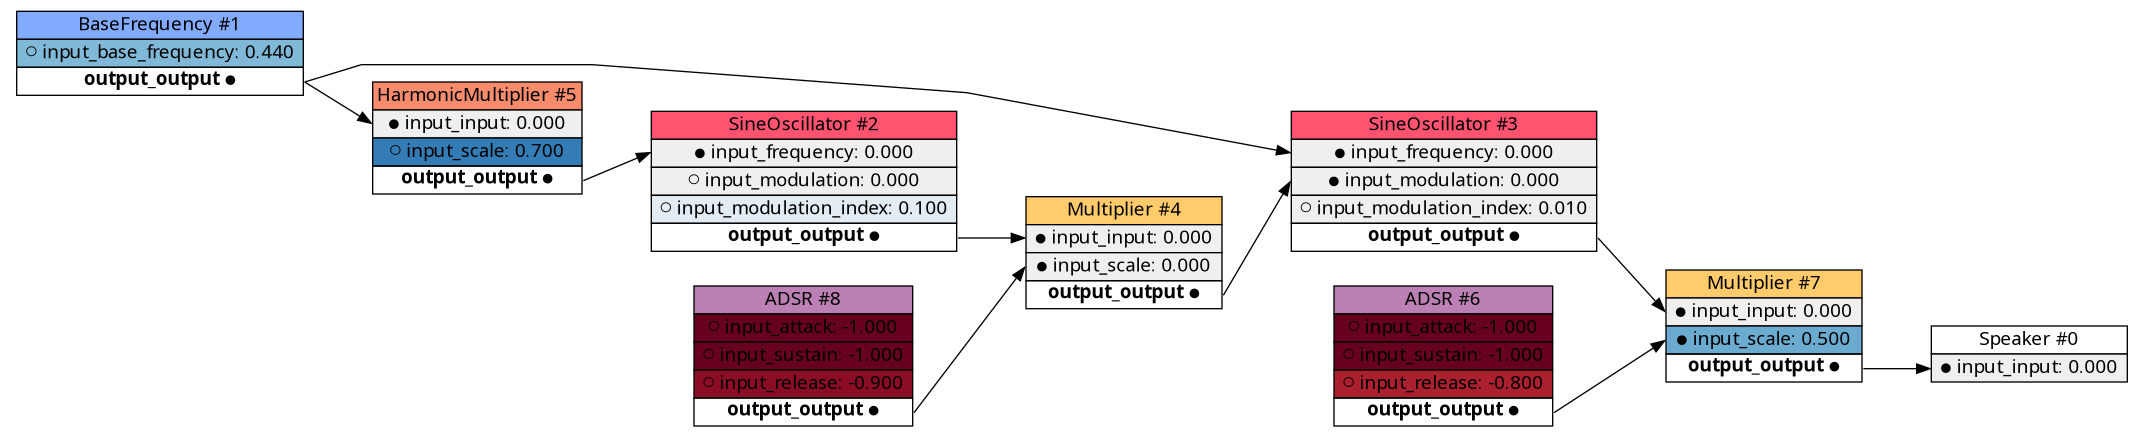
\includegraphics[angle=90,width=0.29\linewidth]{rys03/fm_graph_for_benchmarks.png}
    \caption{
      Prosty graf syntezy FM, zawierający jeden oscylator służący za sygnał nośny
      i jeden oscylator służący za sygnał modulujący.
    }
\end{figure}

Metoda testowania została zaczerpnięta z~\cite{evolutionary_puredata}.
Funkcje celu zostały wpierw przetestowane poprzez wykonanie
zbioru przekrojów przez uproszczony problem syntezy typu FM\@.
Następnie przeprowadzono próby automatycznego dostosowania parametrów dwóch grafów
o predefiniowanej strukturze, dla syntezy FM oraz \textit{analog modeling}.
Ponieważ barwa dźwięku jest odczuciem z natury subiektywnym~\cite{ji2020comprehensive},
ostateczna decyzja dotycząca wyboru funkcji celu została dokonana
przez autora pracy, proces decyzyjny został opisany w
sekcjach~\ref{sec:problem_crossection_results_analysis}
oraz~\ref{sec:fixed_structure_optimisation_results}.

\section{Prezentacja wyników}

Próbki dźwięku (docelowe oraz wygenerowane) zaprezentowane są w pracy w formie
spektrogramów, ponieważ taki format jest najbardziej czytelny dla
człowieka~\cite{computational_music_synthesis}
i pozwala ocenić skuteczność algorytmu optymalizacji.
Inne prace w podobnych dziedzinach również wykorzystują
spektrogramy~\cite{evolutionary_puredata}~\cite{engel2020ddsp}.

\section{Przekrój wartości funkcji celu dla prostego problemu syntezy typu FM}\label{sec:fm_synth_params_cross_section}

Testy obejmowały wygenerowanie wartości funkcji celu podczas
modyfikowania pojedynczego parametru w grafie przetwarzania sygnałów
przedstawionym na rysunku~\ref{fig:fm_graph_for_benchmarks}.
Modyfikowane parametry odpowiadają za różne cechy barwy uzyskanego dźwięku:

\begin{itemize}
  \item \texttt{HarmonicMultiplier/input\_scale}: częstotliwość modulacji FM,
  \item \texttt{SineOscillator/input\_modulation\_index}: siła składowych harmonicznych,
  \item \texttt{ADSR/input\_attack}: dynamika dźwięku.
\end{itemize}


\begin{figure}[H]\label{fig:target_function_testing}
    \centering
    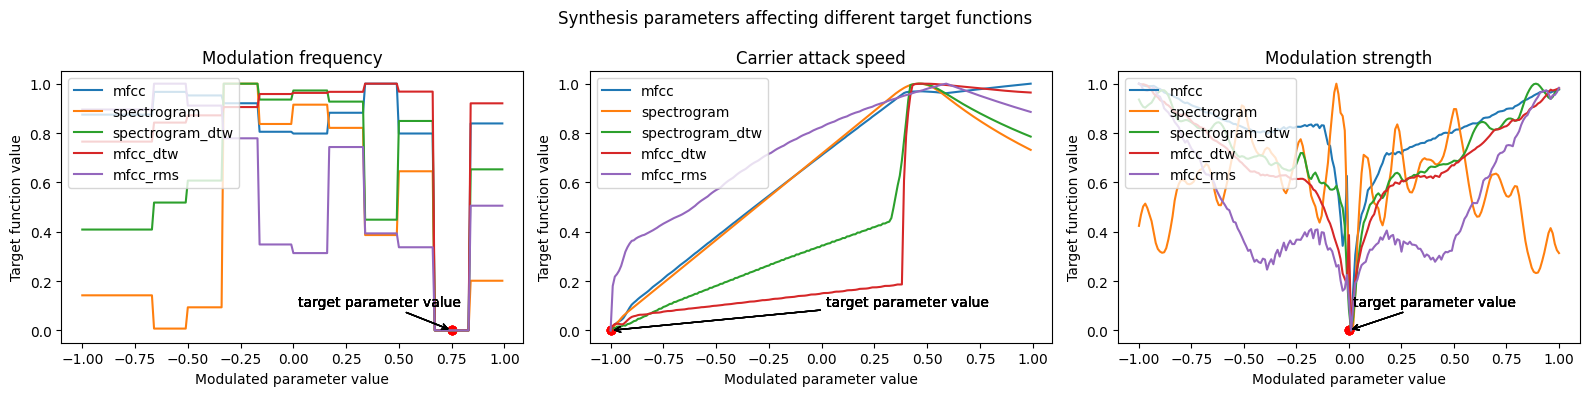
\includegraphics[width=1.0\linewidth]{rys03/target_function_testing.png}
    \caption{
      Zmiany w wartościach testowanych funkcji celu podczas przesuwania różnych parametrów syntezy dźwięku. 
      Kształt pierwszego wykresu wynika z zastosowania kwantyzacji dostępnych częstotliwości modulacji,
      aby wykluczyć nieharmoniczne stosunki częstotliwości modulacji i nośnej. Tego rodzaju praktyka
      jest wykorzystywana w syntezatorach FM~\cite{digitone_manual}, ponieważ ułatwia dostosowywanie parametrów syntezy.
    }
\end{figure}

\subsection{Analiza wyników}\label{sec:problem_crossection_results_analysis}

Wyniki testów zaprezentowane na wykresach~\ref{fig:target_function_testing} pozwalają na
wyeliminowanie różnicy między spektrogramami jako funkcji celu,
ponieważ w przypadku zmian częstotliwości modulacji posiada ona minimum globalne w 
niewłaściwej pozycji parametru. Późniejsze testy wykorzystują tylko funkcje celu
wykorzystujące MFCC\@.

\subsubsection{Częstotliwość modulacji FM}

Wszystkie funkcje z wyjątkiem różnicy między spektrogramami pokazują poprawną, 
najniższą wartość dla właściwej wartości parametru.

\subsubsection{Dynamika dźwięku}

W przypadku wpływu zmian w dynamice dźwięku na wartości funkcji celu,
zastosowanie DTW znacząco zmienia kształt funkcji celu, zależnie od wybranego rozmiaru
okna DTW\@. Duży rozmiar okna powoduje zmniejszenie kary za niedokładne odwzorowanie
dynamiki dźwięku. 

\subsubsection{Siła modulacji}

Różnica między spektrogramami jest najbardziej chaotyczna, nie maleje wraz
ze zbliżaniem się do poprawnej wartości parametru. Pozostałe funkcje celu
wykorzystujące \textit{MFCC} mają lepszą charakterystykę -- maleją
wraz ze zbliżaniem się do poprawnej wartości parametru.

\section{Optymalizacja parametrów dla predefiniowanych
grafów syntezy FM oraz \textit{analog modeling}}

Drugą częścią procesu testowania funkcji celu z literatury było zweryfikowanie skuteczności
każdej z funkcji w uproszczonym problemie optymalizacyjnym, polegającym jedynie na odnalezieniu właściwych
parametrów dla predefiniowanej struktury grafu DSP\@. Wykorzystano dwa grafy
DSP~(rysunki~\ref{fig:analog_graph_for_benchmarks} i~\ref{fig:fm_graph_for_benchmarks}),
wykonujące różne rodzaje syntezy.

\subsection{Synteza FM}

Testowana struktura grafu wykonującego syntezę typu FM~\ref{fig:fm_graph_for_benchmarks}
wykorzystuje 2 operatory: jedną nośną
i jeden modulator. Parametry grafu zostały ręcznie dostrojone aby wygenerować krótki
dźwięk typu \textit{pluck}, w którym modulator przekształca nośną sinusoidę w sygnał zbliżony
do sygnału prostokątnego. Z perspektywy wynikowego spektrum sygnału, przedstawionego na
rysunku~\ref{fig:param_optimisation_results_spectrograms} sygnał składa się z częstotliwości
podstawowej i jednej składowej harmonicznej. Wizualizacja sygnału została przedstawiona
na wykresie~\ref{fig:fm_training_sample_overview}.

\begin{figure}[H]
    \centering
    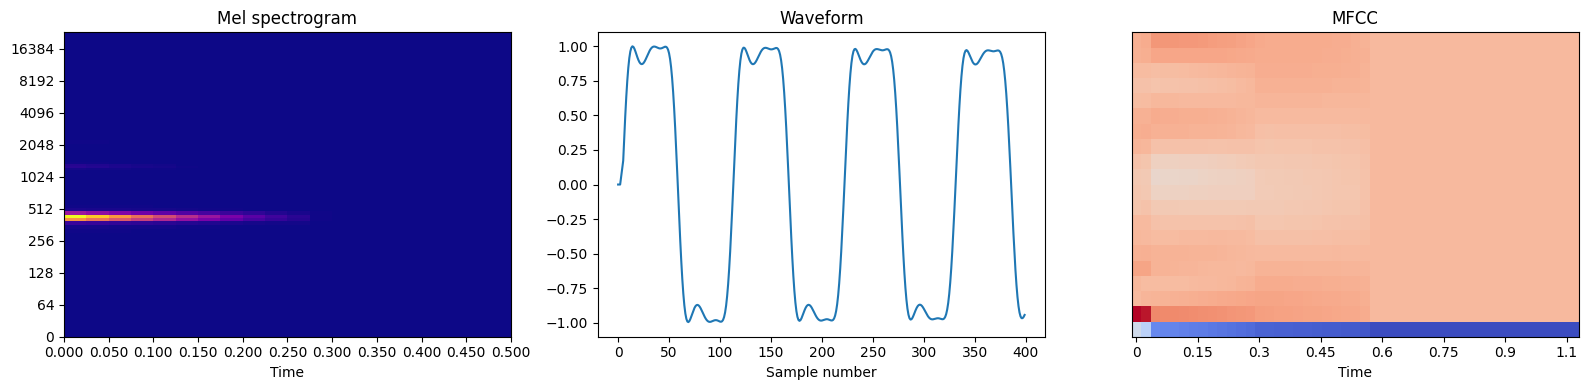
\includegraphics[width=1.0\linewidth]{rys03/fm_training_sample_overview.png}
    \caption{
      Spektrogram, kształt fali oraz wizualizacja MFCC dla próbki dźwięku, którą
      ma imitować graf syntezy FM podczas testów różnych funkcji celu.
    }\label{fig:fm_training_sample_overview}
\end{figure}


\subsection{Synteza \textit{analog modeling}}

\begin{figure}
    \centering
    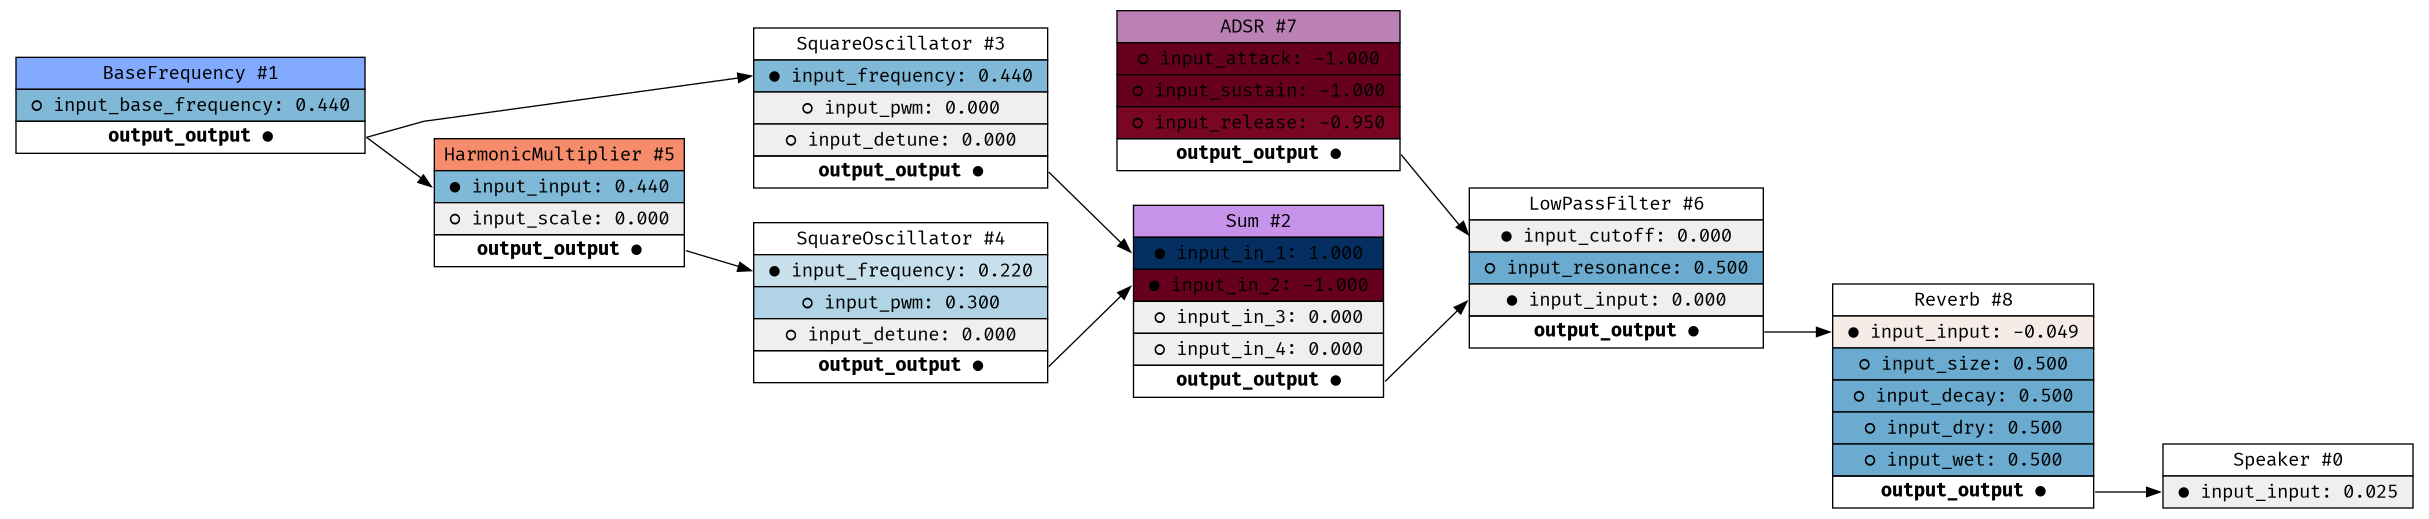
\includegraphics[angle=90, width=0.30\linewidth]{rys03/analog_graph_for_benchmarks.png}
    \caption{
      Graf wykonujący syntezę typu \textit{analog modeling}, wykorzystany do testów funkcji celu.
    }\label{fig:analog_graph_for_benchmarks}
\end{figure}

Synteza \textit{analog modeling} zazwyczaj wykorzystuje mniej parametrów niż synteza
FM~(\ref{fig:fm_graph_for_benchmarks}), aby zwiększyć trudność problemu optymalizacyjnego
graf został roszszerzony o węzeł dodający efekt pogłosu~\cite{reverb}.
Struktura grafu (przedstawiona na rysunku~\ref{fig:analog_graph_for_benchmarks}) składa
się z dwóch oscylatorów generujących sygnał prostokątny. Oscylator \texttt{SquareOscillator \#4}
generuje sygnał przesunięty o oktawę w dół w stosunku do częstotliwości podstawowej, jednocześnie
jego parametr \texttt{input\_pwm} skraca szerokość generowanego impulsu, aby wzbogacić barwę dźwięku
o dodatkowe składowe harmoniczne. Barwa dźwięku zmienia się dynamicznie w czasie dzięki 
zastosowaniu filtra niskoprzepustowego (\texttt{LowPassFilter \#6}), którego
częstotliwość odcięcia jest modulowana przez sygnał sterujący \texttt{ADSR \#7}.
Długość dźwięku generowanego przez oscylatory jest podobna jak w przypadku
grafu FM~(\ref{fig:fm_graph_for_benchmarks}), zastosowanie węzła \texttt{Reverb \#8}
przedłuża czas trwania dźwięku i dodatkowo~,,rozmywa go'' w czasie, co pokazuje
spektrum sygnału na wykresie~\ref{fig:am_training_sample_overview}.

\begin{figure}[H]
  \centering
  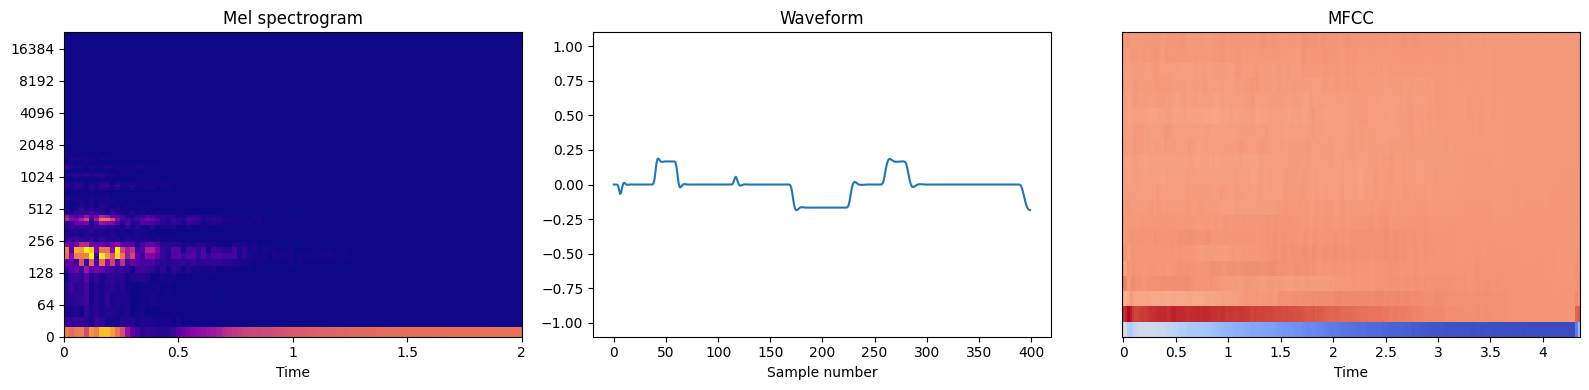
\includegraphics[width=1.0\linewidth]{rys03/am_training_sample_overview.png}
  \caption{
    Spektrogram, kształt fali oraz wizualizacja MFCC dla próbki dźwięku, którą
    ma imitować graf syntezy \textit{analog\_modeling} podczas testów różnych funkcji celu.
  }\label{fig:am_training_sample_overview}
\end{figure}



\subsection{Plan testów}

Dla obu grafów wykonano optymalizację parametrów wejściowych w celu imitacji danej
próbki dźwięku. Optymalizację wykonano 10 razy dla każdej rozważanej~(\ref{sec:considered_target_functions})
funkcji celu. Do optymalizacji parametrów wykorzystano algorytm evolucyjny
\textit{differential evolution}~\cite{2020SciPy-NMeth}. 
Zastosowano następujące parametry algorytmu genetycznego:

\begin{enumerate}
  \item liczba iteracji: \texttt{200},
  \item rozmiar populacji: \texttt{40},
  \item strategia mutacji: \texttt{best1bin},
  \item rekombinacja: \texttt{0.7}.
\end{enumerate}


\subsection{Wyniki testów}\label{sec:fixed_structure_optimisation_results}

\begin{figure}[H]
    \centering
    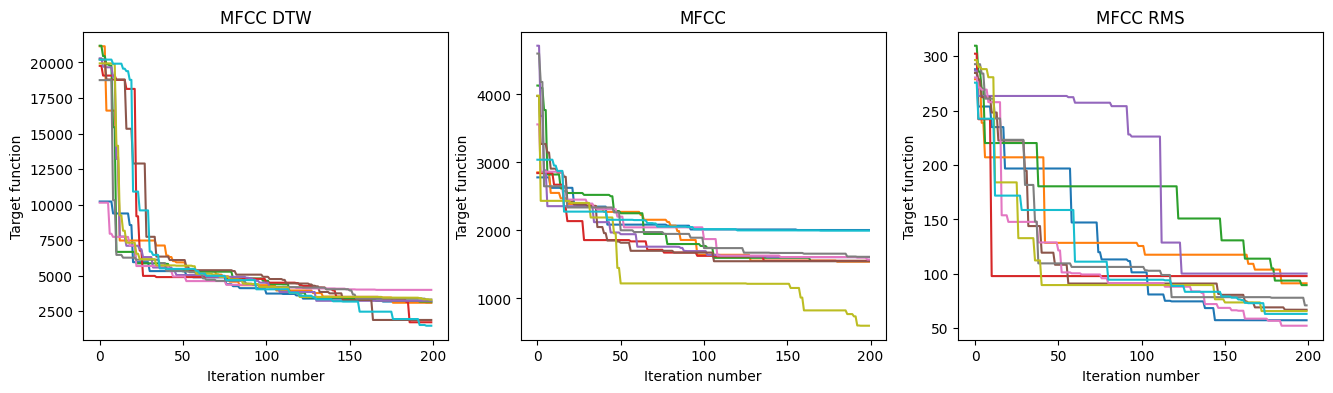
\includegraphics[width=1.0\linewidth]{rys03/target_functions_progress.png}
    \caption{
      Wykresy zmian funkcji celu podczas optymalizacji dla grafu syntezy FM\@.
    }\label{fig:param_optimisation_results_target_fun_plots}
\end{figure}

\begin{figure}[H]
    \centering
    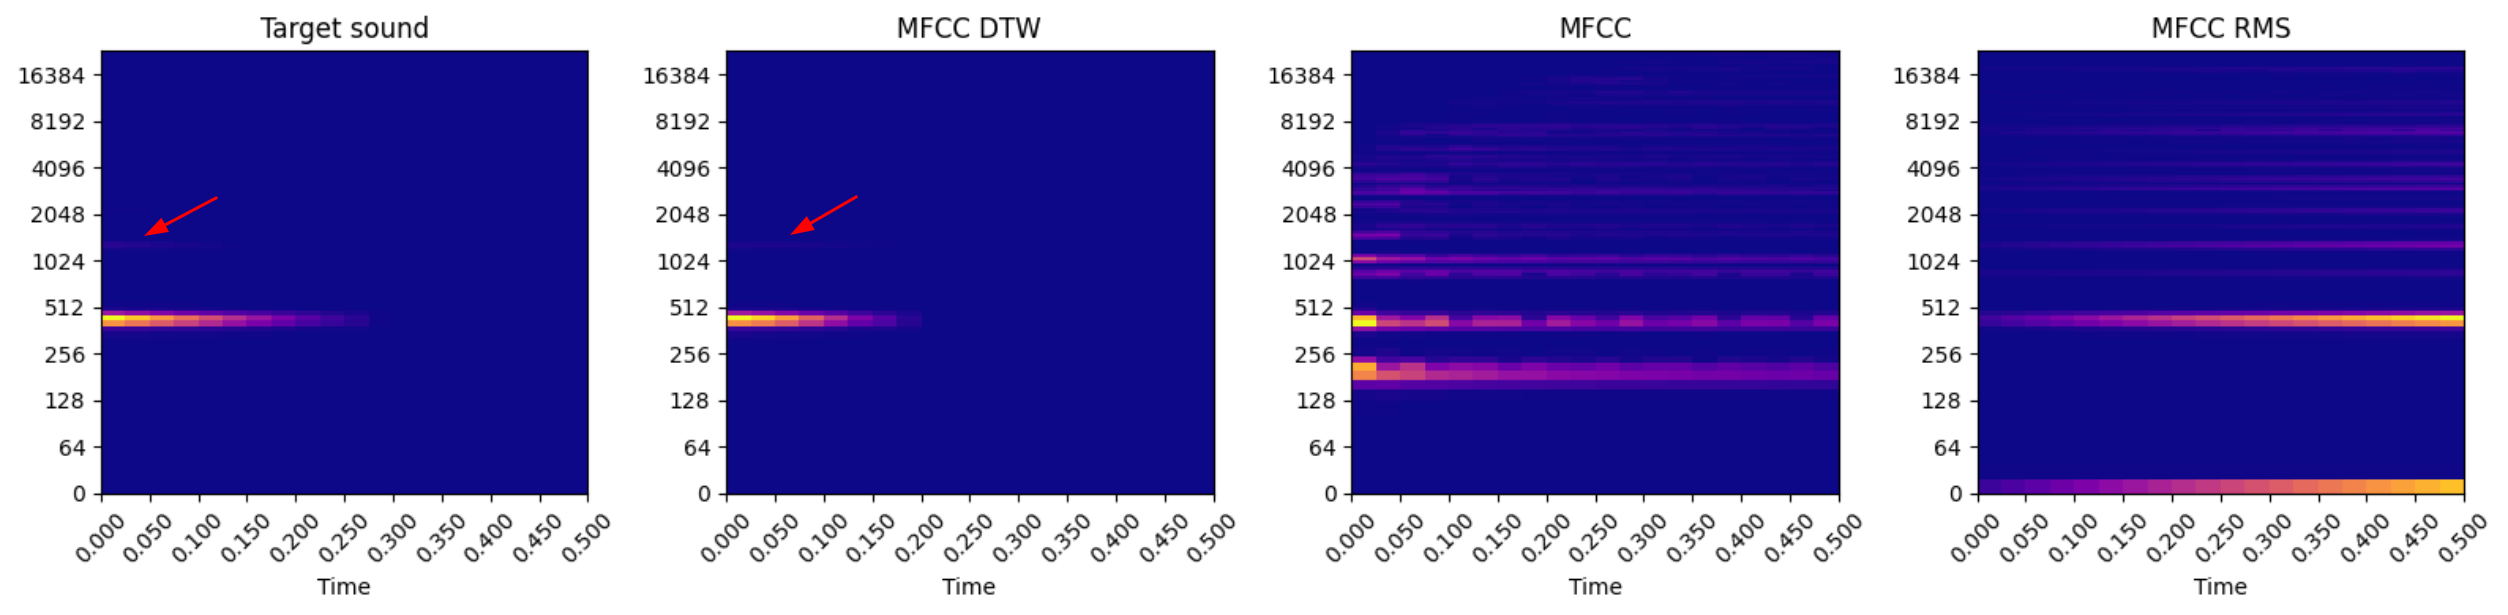
\includegraphics[width=1.0\linewidth]{rys03/spectro_results_fm.png}
    \caption{
      Spektrogram dźwięku docelowego oraz dźwięków uzyskanych w procesie optymalizacji parametrów grafu FM\@.
      Czerwoną strzałką oznaczono składową harmoniczną (słabo widoczną na spektrogramie),
      która została poprawnie odtworzona przez algorytm optymalizacji.
    }\label{fig:param_optimisation_results_spectrograms}
\end{figure}

\subsubsection{Synteza FM}

Algorytm optymalizacji jest w stanie poprawnie dostosować wartości parametrów grafu w przypadku
zastosowania MFCC+DTW jako funkcji celu. Jak pokazuje spektrogram~(\ref{fig:param_optimisation_results_spectrograms}),
poprawnie odtworzona jest zarówno dynamika dźwięku i składowa harmoniczna. Pozostałe funkcje celu nie pozwalają
na odtworzenie sygnału, który w bliski sposób przypomina dźwięk docelowy, pomimo uzyskiwania wyników zbliżonych
do MFCC+DTW we wcześniejszych testach~(\ref{sec:fm_synth_params_cross_section}).

\subsubsection{Synteza \textit{analog modeling}}

\begin{figure}[H]
    \centering
    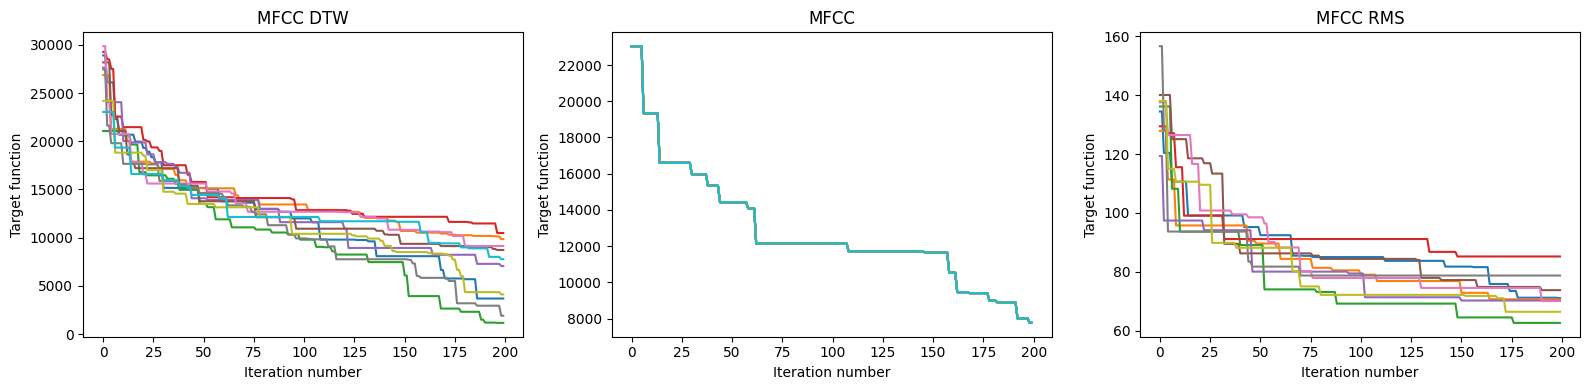
\includegraphics[width=1.0\linewidth]{rys03/am_training_results.png}
    \caption{
      Wykresy zmian funkcji celu podczas optymalizacji dla grafu syntezy \textit{analog modeling}.
    }\label{fig:am_target_fun_plots}
\end{figure}

\begin{figure}[H]
    \centering
    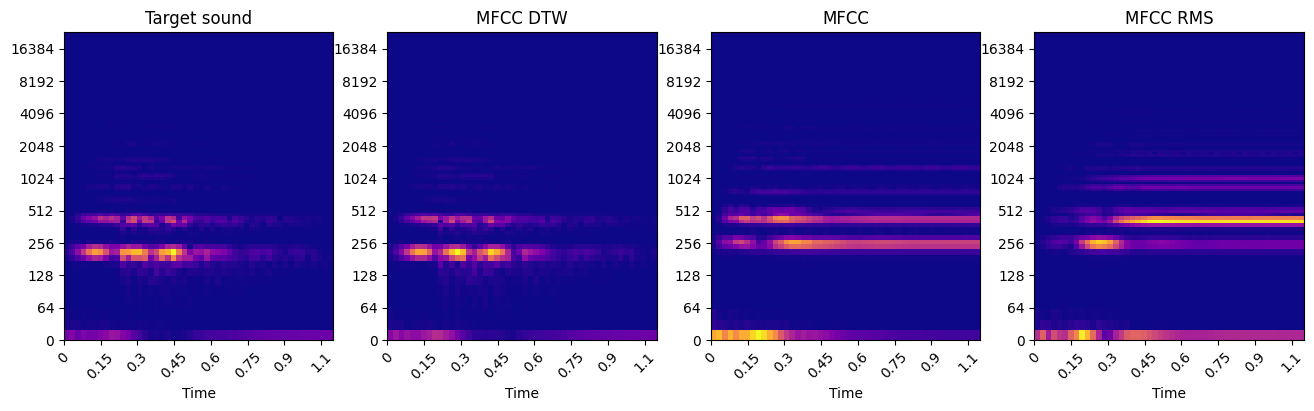
\includegraphics[width=1.0\linewidth]{rys03/spectro_results_am.png}
    \caption{
      Spektrogram dźwięku docelowego oraz dźwięków uzyskanych w procesie
      optymalizacji parametrów grafu \textit{analog modeling}.
    }\label{fig:am_param_optimisation_results_spectrograms}
\end{figure}

Podobnie jak podczas testów syntezy FM, funkcja celu MFCC+DTW pozwala na dokładne odwzorowanie barwy dźwięku.
Na spektrogramie~\ref{fig:am_param_optimisation_results_spectrograms} widoczne są poprawnie odtworzone
składowe harmoniczne, przebieg dynamiczny dźwięku oraz parametry efektu pogłosu. Funkcja celu wykorzystująca
tylko współczynniki MFCC nie jest w stanie odtworzyć przebiegu dynamicznego dźwięku i jedynie częściowo odtwarza
poprawne składowe harmoniczne. MFCC+RMS nie jest w stanie odtworzyć żadnej z cech docelowego dźwięku.

\subsection{Wybór funkcji celu na podstawie wyników}

Wyniki testów pozwalają jednoznacznie wybrać funkcję celu, która porównuje wartości MFCC
sygnałów za pomocą algorytmu \textit{dynamic time warping}. W zakresie pracy nie leży szczegółowe
wytłumaczenie, czemu zastosowanie DFT usprawnia proces optymalizacji. Możliwym intuicyjnym
wytłumaczeniem tego fenomenu jest fakt, że DFT pozwala na rozpoznanie poszczególnych
fonemów w nagraniach mowy~\cite{mfcc_dtw}, niezależnie od prędkości wypowiadania słów. 
Analogicznie, w przypadku porównywania sygnałów dźwiękowych generowanych przez grafy
przetwarzania sygnałów, wykorzystanie DFT może powodować~,,wygładzenie'' niedokładności
w zmianach tembru (transjentach~\cite{transient_music_theory}) i dynamiki dźwięku,
które występują pomiędzy sygnałem docelowym i wygenerowanym.

\chapter{Algorytm rozwiązania}\label{chap:solution_algorithm}

\begin{figure}[H]    
    \centering
    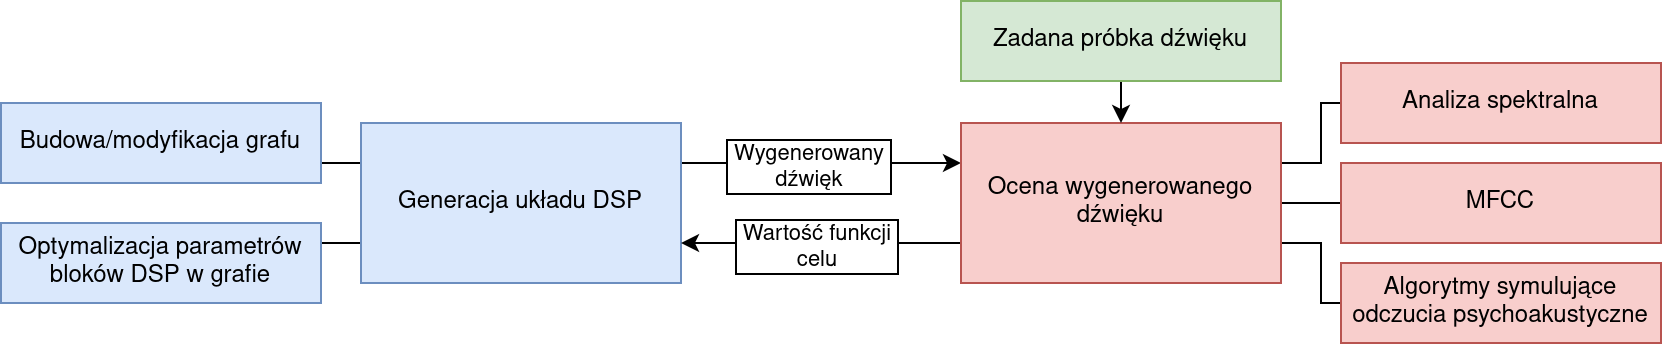
\includegraphics[width=1.0\linewidth]{rys04/solution_algorithm_diagram.png}
    \caption{
      Diagram algorytmu rozwiązania zaimplementowanego w ramach pracy.
      Algorytm oceny może wykorzystywać różne funkcje celu, finalnie zastosowano
      MFCC oraz \textit{dynamic time wrapping},
      proces wyboru funkcji celu opisuje rozdział~\ref{target_function_chapter}.
    }\label{fig:solution_algorithm_diagram}
\end{figure}

Jak opisano w rozdziale poświęconym definicji problemu~(\ref{chap:problem_definition}), praca
rozwiązuje problem budowy grafu DSP z wykorzystaniem dwóch algorytmów:
\begin{enumerate}
  \item Algorytm generujący graf DSP, opisany w rozdziale~\ref{dsp_graph_chapter},
  \item Algorytm oceniający jak bardzo wygenerowany dźwięk jest bliski dźwiękowi docelowemu pod względem barwy,
    opisany w rozdziale~\ref{target_function_chapter}.
\end{enumerate}

Praca wykorzystuje algorytm genetyczny, w którym genotyp odpowiada za strukturę grafu oraz wartości
przypisane do parametrów grafu~(\ref{eq:graph_structure_generation_function},~\ref{eq:graph_params_assignment}).
Diagram blokowy~\ref{fig:solution_algorithm_diagram} ilustruje zaimplementowany algorytm.

\chapter{Analiza wyników, możliwe drogi dalszego rozwoju} \label{results_analysis_chapter}
% \section{Zasady redakcji}
% W pracy należy dbać o poprawność redakcyjną zgodnie z zaleceniami:
% \begin{itemize}
% \item nie zostawiać znaku spacji przed znakami interpunkcji (zamiast ,,powiedziano , że ...'' powinno być ,,powiedziano, że ...''),
% \item kropki po skrótach, które nie są jednocześnie kropkami kończącymi zdanie sklejać z kolejnym wyrazem znakiem tyldy, np.~jak tutaj (\verb?np.~jak tutaj?) lub wstawiać za nimi ukośnik, np.\ jak tutaj (\verb?np.\ jak tutaj?),
% \item nie zapominać o formatowaniu wyliczenia (należy zaczynać małymi literami lub dużymi oraz kończyć przecinkami, średnikami i kropkami -- w zależności od kontekstu danego wyliczenia),
% \item nie zostawiać samotnych literek na końcach linii  (można je ,,skleić'' z wyrazem następnym stosując znaczek tyldy, jak \verb+w~przykładzie+),
% \item nie zostawiać pojedynczych wierszy na końcu lub początku strony (należy kontrolować ,,sieroty'' i ,,wdowy''),
% \item nie zostawiać odstępu pomiędzy tekstem a nawiasami czy znakami cudzysłowów (znaki te powinny przylegać do tekstu, który obejmują ,,jak w tym przykładzie''),
% \item wyrazy obcojęzyczne powinny być pisane czcionką pochyłą (preferowane \verb|\emph{}|) wraz ze skrótem oznaczającym język, w szczególności ma to zastosowanie przy rozwijaniu skrótów, np.~OGC (ang.~\emph{Open Geospatial Consortium}) (w kodzie latexowym wygląda to tak: \verb|np.~OGC (ang.~\emph{Open Geospatial Consortium})|),
% \item każdy zastosowany skrót powinien zostać rozwinięty podczas pierwszego użycia, później może już występować bez rozwinięcia (skrót i jego rozwinięcie powinny trafić również do wykazu \emph{Skróty}, jeśli taki wykaz jest dołączany do dokumentu),
% \item nie wolno zostawiać zbyt dużo białej przestrzeni bez żadnego uzasadnienia. 
% \end{itemize}

% Odnosząc się do ostatniej zasady, to przekłada się ona na gospodarowanie białą przestrzenią. Poniżej przedstawiono przykład złego użycia listy wyliczeniowej. Jeśli bowiem elementy na liście są reprezentowane przez krótki tekst, to wtedy powstaje biała plama. Widać to szczególnie przy długich listach.
% \begin{quotation}
% 	\noindent Moje ulubione kolory to:
% 	\begin{itemize}
% 	\item biały,
% 	\item niebieski,
% 	\item czerwony.
% 	\end{itemize}
% \end{quotation}

% Dużo lepiej w takim przypadku albo po prostu wyliczyć wartości po przecinkach:
% \begin{quotation}
% 	\noindent Moje ulubione kolory to: biały, niebieski, czerwony.
% \end{quotation}
% albo wypisać listę w kilku kolumnach:
% \begin{quotation}
% 	\noindent Moje ulubione kolory to:
% \begin{multicols}{3}
% 	\begin{itemize}
% 	\item biały,
% 	\item niebieski,
% 	\item czerwony.
% 	\end{itemize}
% \end{multicols}
% \end{quotation}



% \section{Rysunki}
% W niniejszym szablonie numeracja rysunków odbywa się automatycznie według następujących reguł: rysunki powinny mieć numerację ciągłą w obrębie danego rozdziału, sam zaś numer powinien składać się z dwóch liczb rozdzielonych kropką. Pierwsza liczbą ma być numer rozdziału, drugą -- kolejny numer rysunku w rozdziale. Przykładowo: pierwszy rysunek w rozdziale 1 powinien mieć numer 1.1, drugi -- numer 1.2 itd., pierwszy rysunek w rozdziale 2 powinien mieć numer 2.1, drugi -- numer 1.2 itd. Wszystko to załatwia szablon. 

% Rysunki powinny być wyśrodkowane na stronie wraz z podpisem umieszczonym na dole. Podpisy nie powinny kończyć się kropką. Czcionka podpisu powinna być mniejsza od czcionki tekstu wiodącego o 1 lub 2 pkt (w szablonie jest to czcionka rozmiaru \texttt{small}). Ponadto należy zachowywać odpowiedni odstęp między rysunkiem, podpisem rysunku a tekstem rozdziału. Przykłady, jak to zrobić, zamieszczono w szablonie.

% W~przypadku korzystania z szablon odstępy te regulowane są automatycznie. Podpis i grafika muszą stanowić jeden obiekt. Chodzi o to, że w edytorach tekstu typu Office podpis nie scala się z grafiką i czasem trafia na następną stronę, osieracając grafikę. Korzystającym z niniejszego szablonu i otoczenia \verb?\figure? takie osierocenie nigdy się nie zdarzy.  

% Do każdego rysunku musi istnieć odwołanie w tekście (inaczej mówiąc: niedopuszczalne jest wstawienie do pracy rysunku bez opisu). Odwołania do rysunków powinny mieć postać: ,,Na rysunku~3.3 przedstawiono...'' lub ,,... co ujęto na odpowiednim schemacie (rys.~1.7)''. 

% Jeśli odwołanie stanowi część zdania, to wtedy wyraz ,,rysunek'' powinien pojawić się w całości. Jeśli zaś odwołanie jest ujęte w nawias (jak w przykładzie), wtedy należy zastosować skrót ,,rys.''. Jeśli do stworzenia obrazka wykorzystano jakieś źródła, to powinny one być zacytowane w podpisie tegoż rysunku. 

% Należy pamiętać o tym, że ,,rysunki'' to twory nieżywotne. W związku z tym nie mogą ''pokazywać''. Dlatego ,,rysunek~1.1 pokazuje ...'' jest stylistycznie niepoprawne. Zamiast tego zwrotu trzeba użyć ,, na rysunku~1.1 pokazano ...''.

% Rysunki można wstawiać do pracy używając polecenia \verb|\includegraphics|. Zalecane jest, aby pliki z grafikami były umieszczane w katalogach 
% odpowiadających numerom rozdziałów czy literom dodatków: \verb|rys01|, \verb|rysA| itd. Sposób wstawiania rysunków do pracy zademonstrowano na przykładze rysunków~\ref{fig:kanji-giri} i \ref{fig:alfabeta}.

% \begin{lstlisting}[label=list:includegraphics,caption=Kod źródłowy przykładów wstawiania rysunków do pracy,basicstyle=\footnotesize\ttfamily]
% \begin{figure}[ht]
%  \centering
%   
\includegraphics[width=0.3\linewidth]{rys05/kanji-giri}
%  \caption{Dwa znaki kanji - giri}
%  \label{fig:kanji-giri}
% \end{figure}

% \begin{figure}[htb]
%  \centering
%   \begin{tabular}{@{}ll@{}}
%   a) & b) \\
%   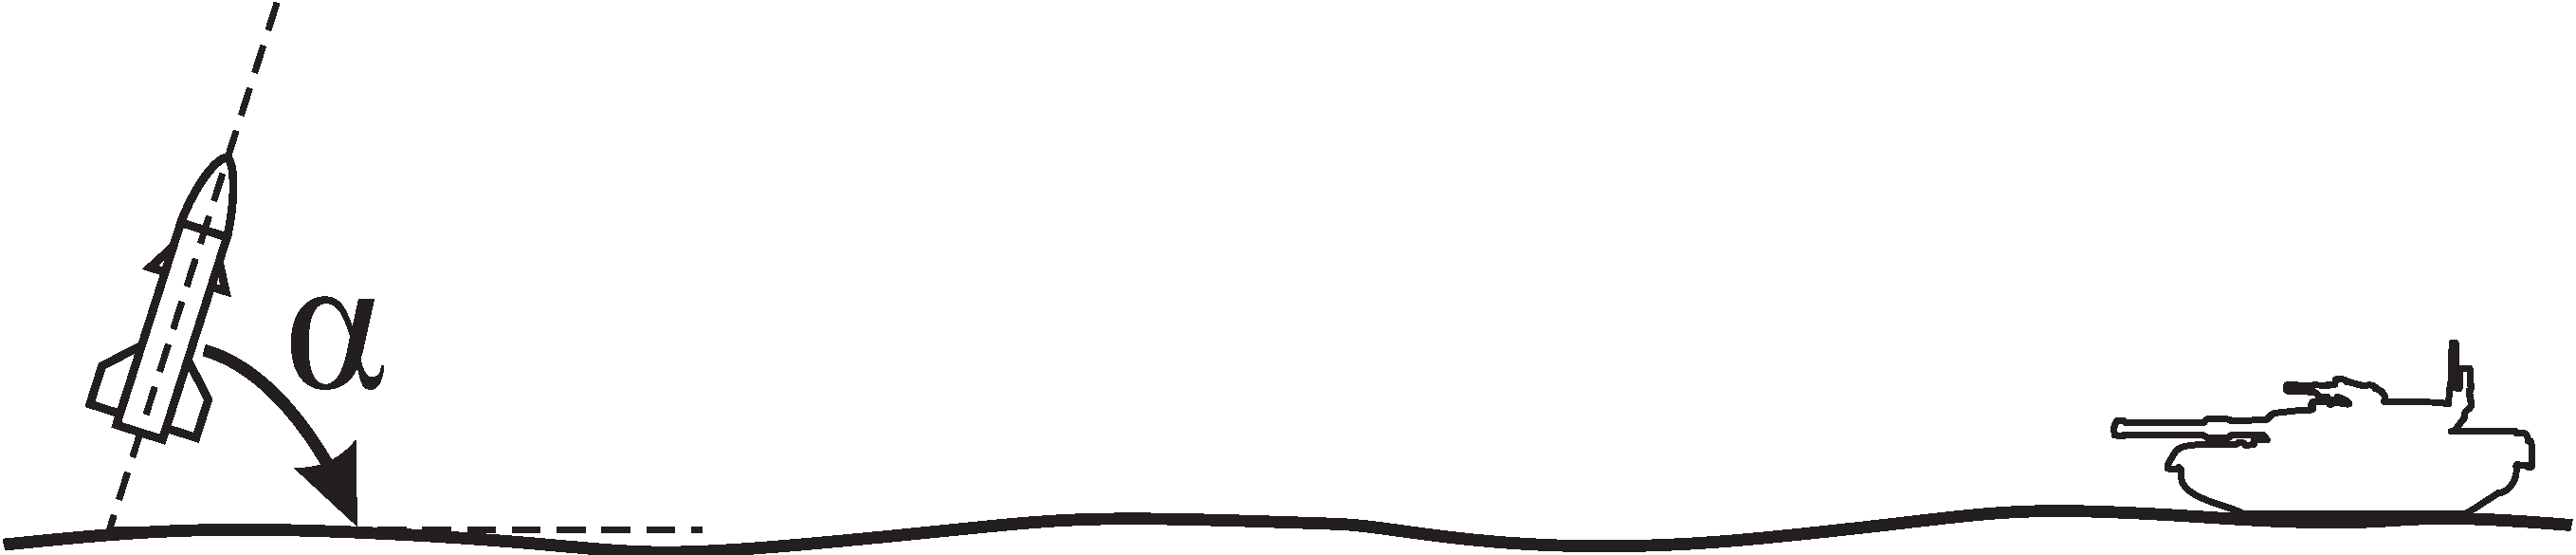
\includegraphics[width=0.475\textwidth]{rys05/alfa1} & 
%   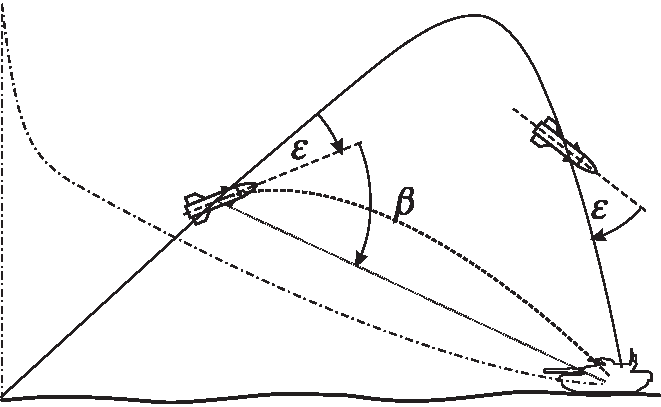
\includegraphics[width=0.475\textwidth]{rys05/beta1}
% 	% jeśli obraki są różnej wysokości, można je wyrównać do góry stosując vtop jak niżej
% 	% \vtop{\vskip-2ex\hbox{{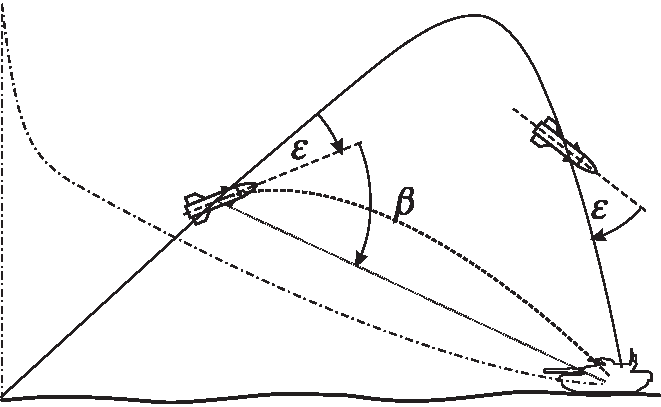
\includegraphics[width=0.475\textwidth]{rys05/beta1}}}} &
% 	% \vtop{\vskip-2ex\hbox{{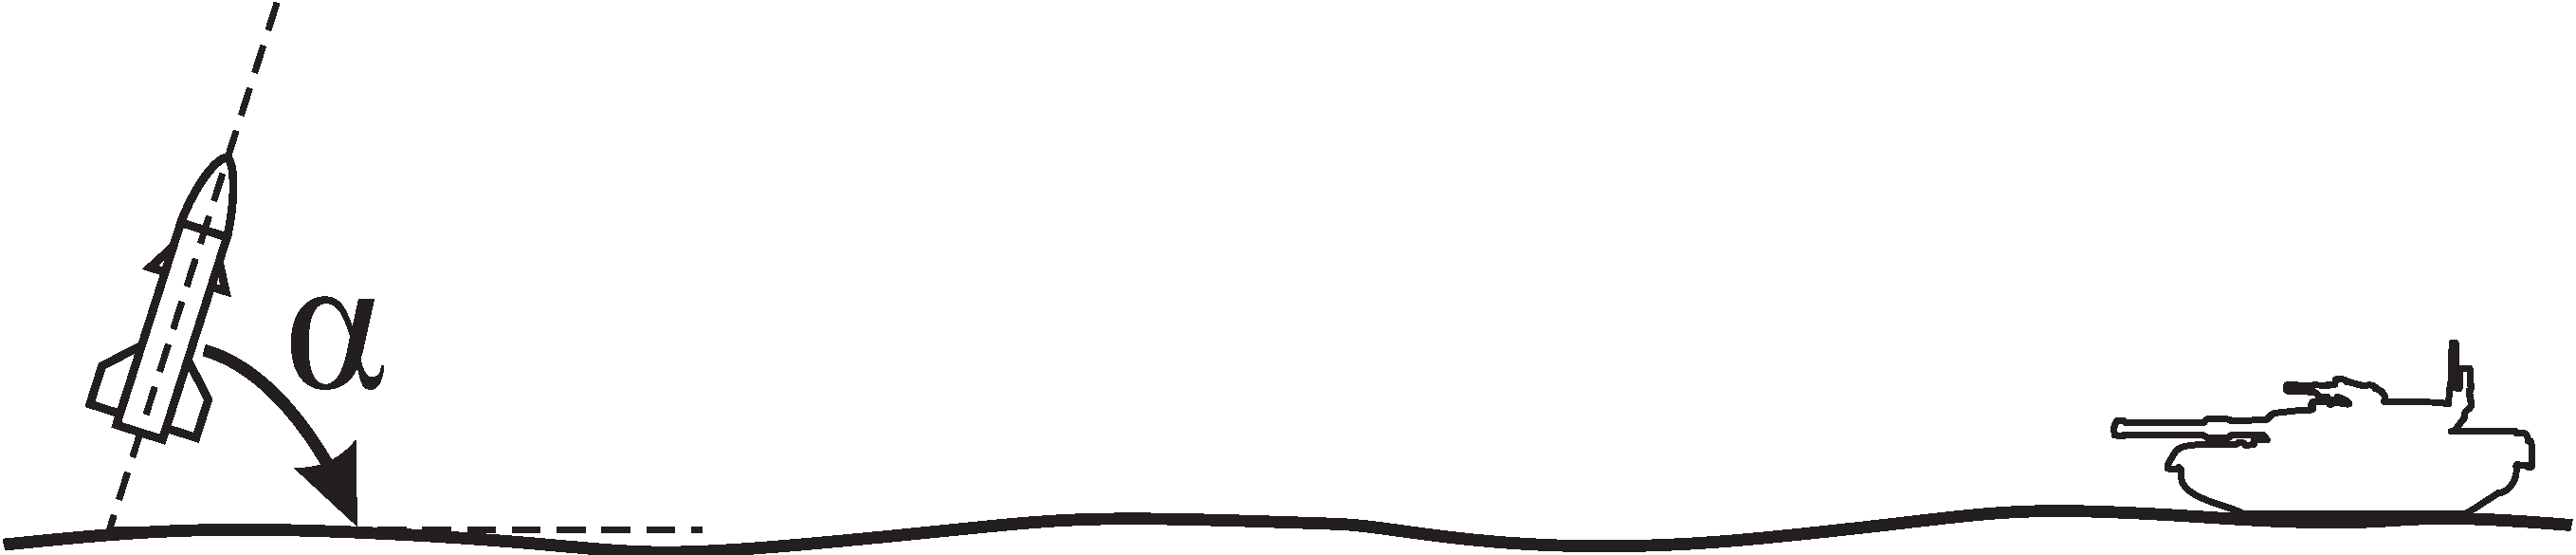
\includegraphics[width=0.475\textwidth]{rys05/alfa1}}}} 
%   \end{tabular}
%  a) trzy podejścia, b) podejście praktyczne}
%  \label{fig:alfabeta}
% \end{figure}
% \end{lstlisting}

% \begin{figure}[ht]
% 	\centering
% 		
\includegraphics[width=0.3\linewidth]{rys05/kanji-giri}
% 	\caption{Dwa znaki kanji -- giri}
% 	\label{fig:kanji-giri}
% \end{figure}

% \begin{figure}[htb]
%   \centering
% 	\begin{tabular}{@{}ll@{}}
% 	a) & b) \\
%   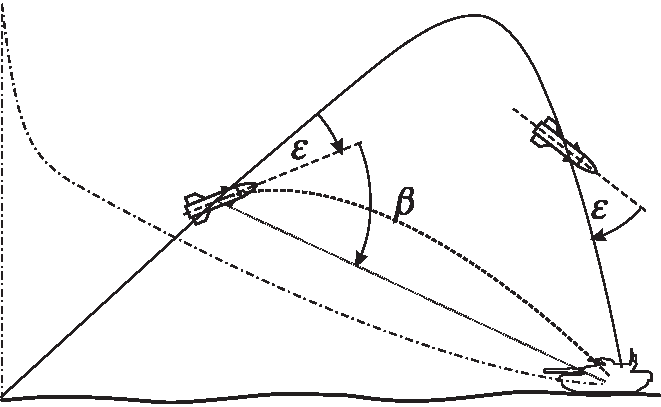
\includegraphics[width=0.475\textwidth]{rys05/beta1} & 
% 	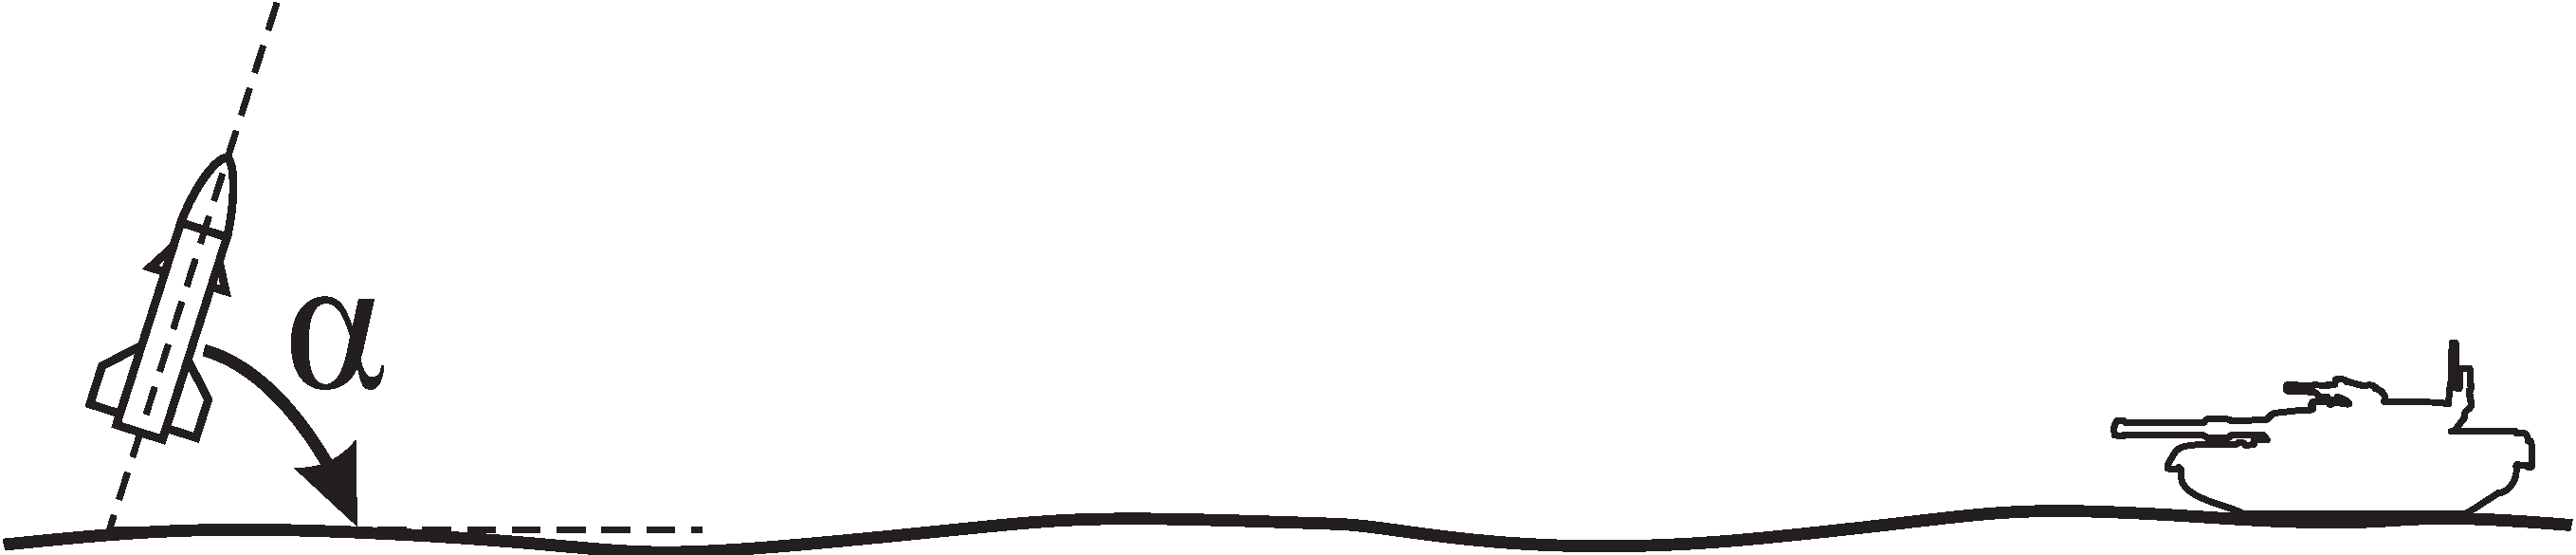
\includegraphics[width=0.475\textwidth]{rys05/alfa1}
% 	% jeśli obraki są różnej wysokości, można je wyrównać do góry stosując vtop jak niżej
% 	% \vtop{\vskip-2ex\hbox{{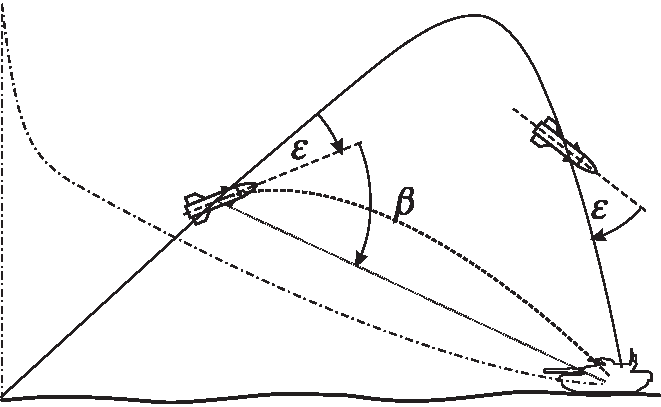
\includegraphics[width=0.475\textwidth]{rys05/beta1}}}} &
% 	% \vtop{\vskip-2ex\hbox{{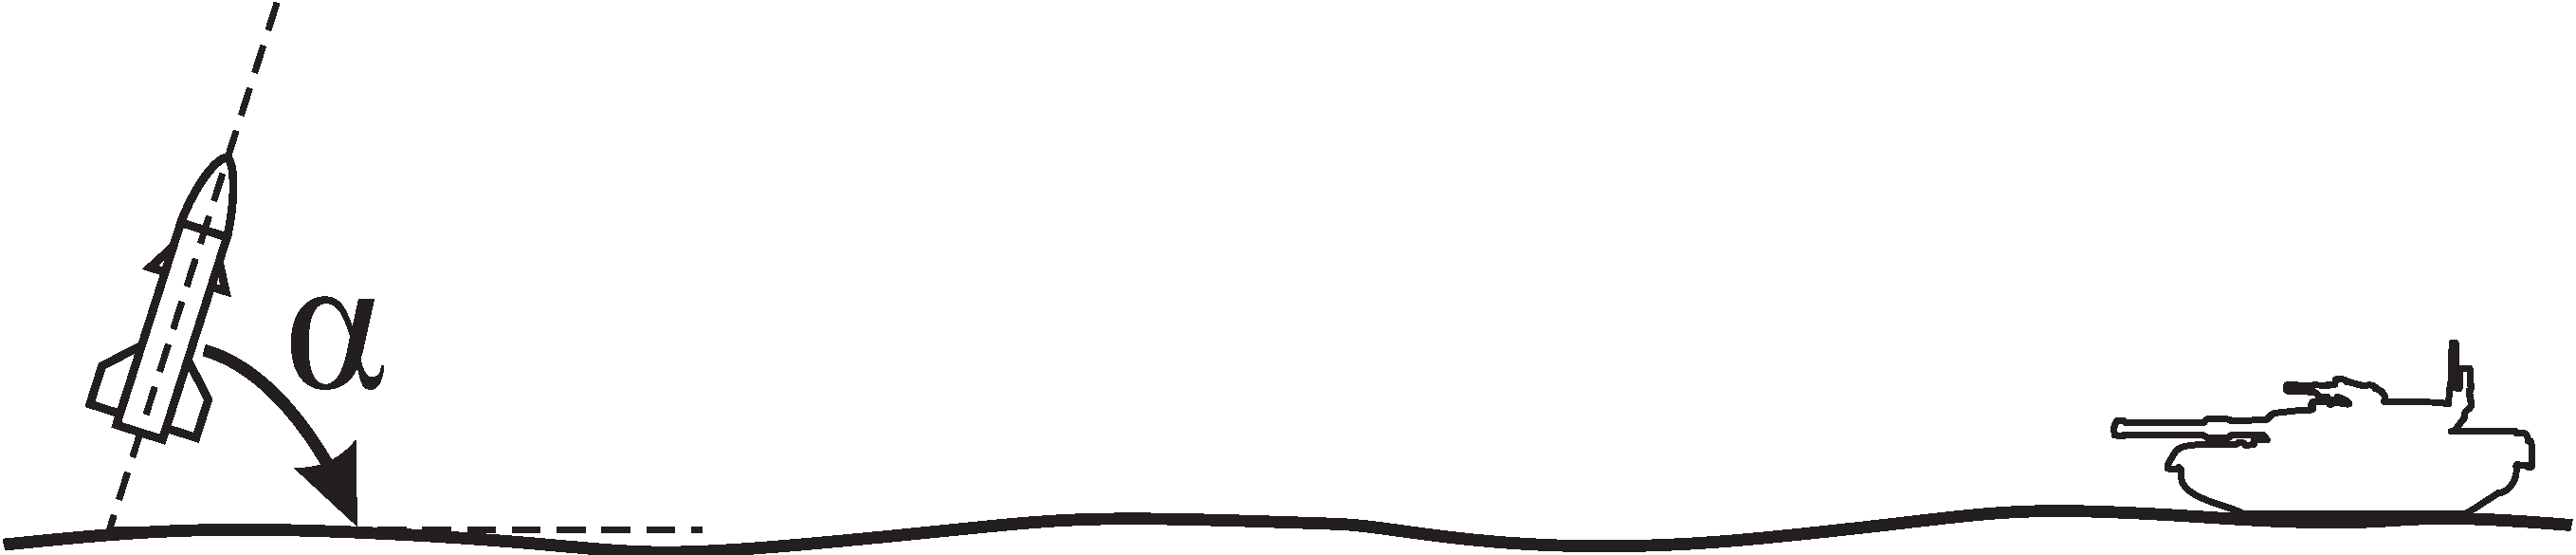
\includegraphics[width=0.475\textwidth]{rys05/alfa1}}}}  \caption{Wyznaczanie trajektorii lotu rakiety: 
% 	\end{tabular}
%   \caption{Wyznaczanie trajektorii lotu rakiety: a) trzy podejścia, b) podejście praktyczne}
%   \label{fig:alfabeta}
% \end{figure}

% Grafiki wektorowe powinny być dostarczone w plikach pdf. Rozmiar strony w~pliku pdf powinien być równy lub minimalnie większy od rozmiaru znajdującej się na nim grafiki (proszę spojrzeć na przykłady grafik wykorzystanych w niniejszym szablonie). Chodzi o to, aby na rysunku nie pojawiała się niepotrzebna biała przestrzeń (rozmiar płótna ma odpowiadać rozmiarowi grafiki bez żadnych marginesów, elementy grafiki powinny być ciasno ułożone). Grafiki rastrowe (głównie zrzuty z ekranu bądź zdjęcia) powinny być dostarczane w plikach o formacie \texttt{png} z~kompresją bezstratną. Zastosowanie kompresji stratnej, jak \texttt{jpg}, wprowadza niepotrzebne artefakty. Podobnie jak w przypadku grafik wektorowych, grafiki rastrowe nie powinny mieć białych marginesów.

% Niezłym sposobem generowanie ładnej grafiki wektorowej, w szczególności diagramów, jest posłużenie się, kolejno, następującymi darmowymi narzędziami:
% \begin{itemize}
% \item w \texttt{diagrams.net} (dawniej \texttt{draw.io}): narysowanie diagramu i wyeksportowanie do pdf (bezpośrednio lub pośrednio, poprzez zapisanie pliku w formacie \texttt{svg}, a potem jego wyświetlenie w~przeglądarce internetowej i wydrukowanie do \texttt{pdf}),
% \item w \texttt{inkscape}: zaimportowanie \texttt{pdf}, rozdzielenie grupy, wykasowanie niepotrzebnych elementów (tła), zaznaczenie wszystkiego, przycięcie strony do zaznaczonych (Ctr-Shift-R), zapisanie jako \texttt{pdf}. 
% \end{itemize}

% Na rysunku~\ref{fig:diagramy} pokazano przykład dobrze i źle (od strony technicznej) narysowanego diagramu. Celowo pokazano ramki, by było widać marginesy. Normalnie ramek tych nie należy stosować.
% \begin{figure}[htb]
%   \centering
% 	\begin{tabular}{@{}ll@{}}
% 	a) & b) \\
%   \vtop{\vskip-2ex\hbox{\fbox{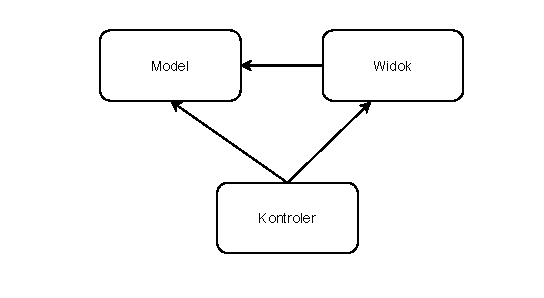
\includegraphics[width=0.4\linewidth]{rys05/diagram1}}}} & 
% 	\vtop{\vskip-2ex\hbox{\fbox{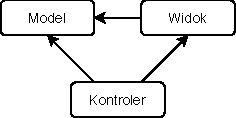
\includegraphics[width=0.4\linewidth]{rys05/diagram2}}}}
% 	% jeśli obraki są różnej wysokości, można je wyrównać do góry stosując vtop jak niżej
% 	% \vtop{\vskip-2ex\hbox{{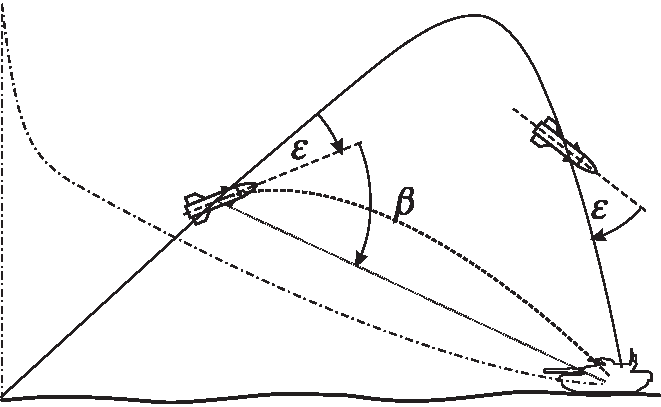
\includegraphics[width=0.475\textwidth]{rys05/beta1}}}} &
% 	% \vtop{\vskip-2ex\hbox{{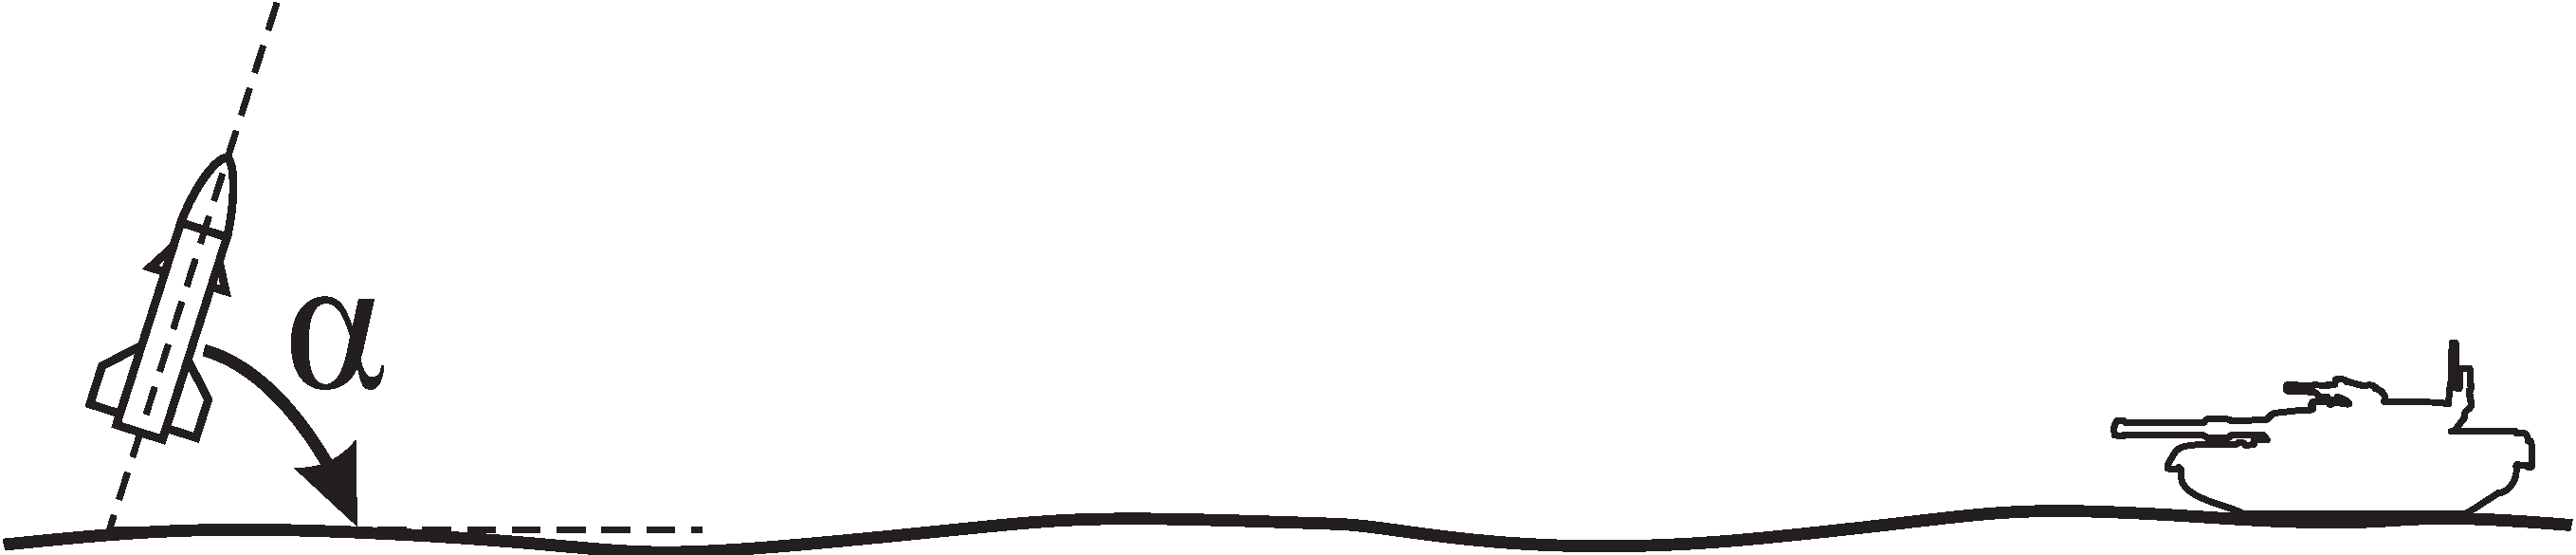
\includegraphics[width=0.475\textwidth]{rys05/alfa1}}}}  \caption{Wyznaczanie trajektorii lotu rakiety: 
% 	\end{tabular}
%   \caption{Przykład diagramu: a) złego, b) w miarę dobrego}
%   \label{fig:diagramy}
% \end{figure}

% Elementy na rysunkach nie powinny być wypełnione 100\% czernią ponieważ na wydrukach tworzą się plamy przebijające się przez kartkę. Zamiast tego wypełnienie elementów powinno być ustawione na ok.\ 90\% czerni.

% Czcionka na rysunkach nie może być większa od czcionki wiodącej tekstu (jedyny wyjątek to np.\ jakieś nagłówki).
% Należy stosować czcionkę kroju Arial, Helvetica bądź tego samego kroju co czcionka dokumentu (\texttt{texgyre-termes}). 

% Jeśli na jednym rysunku pojawić się ma kilka grafik, to zamiast stosować \texttt{subfigure} lub inne otoczenia należy: dostarczyć tabelę z wstawionymi do niej rysunkami, opcjonalnie adnotować jej części (np.~a) i b)), odnieść się do tych części w podpisie (posługując się adnotacjami, jak to zrobiono na rysunkach~\ref{fig:alfabeta} i \ref{fig:diagramy}, lub opisem słownym, np.~,,z lewej strony pokazano ...'', ,,po prawej zamieszczono ...'').

% Jeśli na rysunku zamieszczono w tabeli kilka grafik, to ich pozycjonowaniem (wyjustowaniem od góry) można manipulować za pomocą komendy:
% \verb+\vtop{\vskip-2ex\hbox{\includegraphics[width=0.475\textwidth]{nazwa}}}+

% Na rysunkach nie wolno nadużywać kolorów oraz ozdobników (wiele narzędzi do tworzenia diagramów dostarcza grafikę z cieniowaniem, gradacją kolorów itp.\  co niekoniecznie przekłada się na czytelność rysunku).
% Jeśli rysunki są kolorowe, to kolory te powinny być rozróżnialne po konwersji do poziomów szarości (chodzi o to, aby na wydrukach wykonanych na drukarkach monochromatycznych można było dostrzec różnice).

% Podczas robienia zrzutów z ekranu należy zadbać o to, by taki zrzut był czytelny po wydrukowaniu. Czyli aby pojawiające się literki były wystarczająco duże, a przestrzenie bez treści -- relatywnie małe. Przystępując do robienia zrzutu trzeba odpowiednio wyskalować elementy na ekranie. Na przykład robiąc zrzut z przeglądarki FF najpierw należy wcisnąć CTR--0 (domyślne skalowanie), potem CTR--{}- (zmniejszenie skali o stopień). Potem dobrze jest zawęzić okno przeglądarki tak, by interesująca treść wypełniła je w całości. Jeśli na obserwowanej stronie jest zbyt dużo pustych obszarów, to należy je jakoś zawęzić (sterując wielkością okna przeglądarki lub aktywnymi elementami interfejsu użytkownika). Zrzut bowiem wcale nie musi być odzwierciedleniem 1:1 domyślnego układu obserwowanych elementów. Ważne jest, by na zrzucie pokazać interesujący, opisywany fragment i żeby ten fragment był czytelny. Nie trzeba też zawsze robić zrzutów w układzie 16:9 (lub innym panoramicznym). Czasem lepiej jest zrobić zrzuty okien niemal kwadratowych, bo lepiej się układają w wynikowym dokumencie. Poza tym można je przeskalować (powiększyć) by zajmowały całą szerokość strony, a wtedy czcionka na wydrukach będzie większa. Takie skalowanie dla zrzutów panoramicznych zwykle się nie udaje. Na rysunku~\ref{fig:zrzuty} pokazano przykłady dobrze i źle zrobionych zrzutów (w celu oszczędzenia miejsca zrzuty umieszczono obok siebie).
% 	
% \begin{figure}[htb]
%   \centering
% 	\begin{tabular}{@{}ll@{}}
% 	a) & b) \\
%   \vtop{\vskip-2ex\hbox{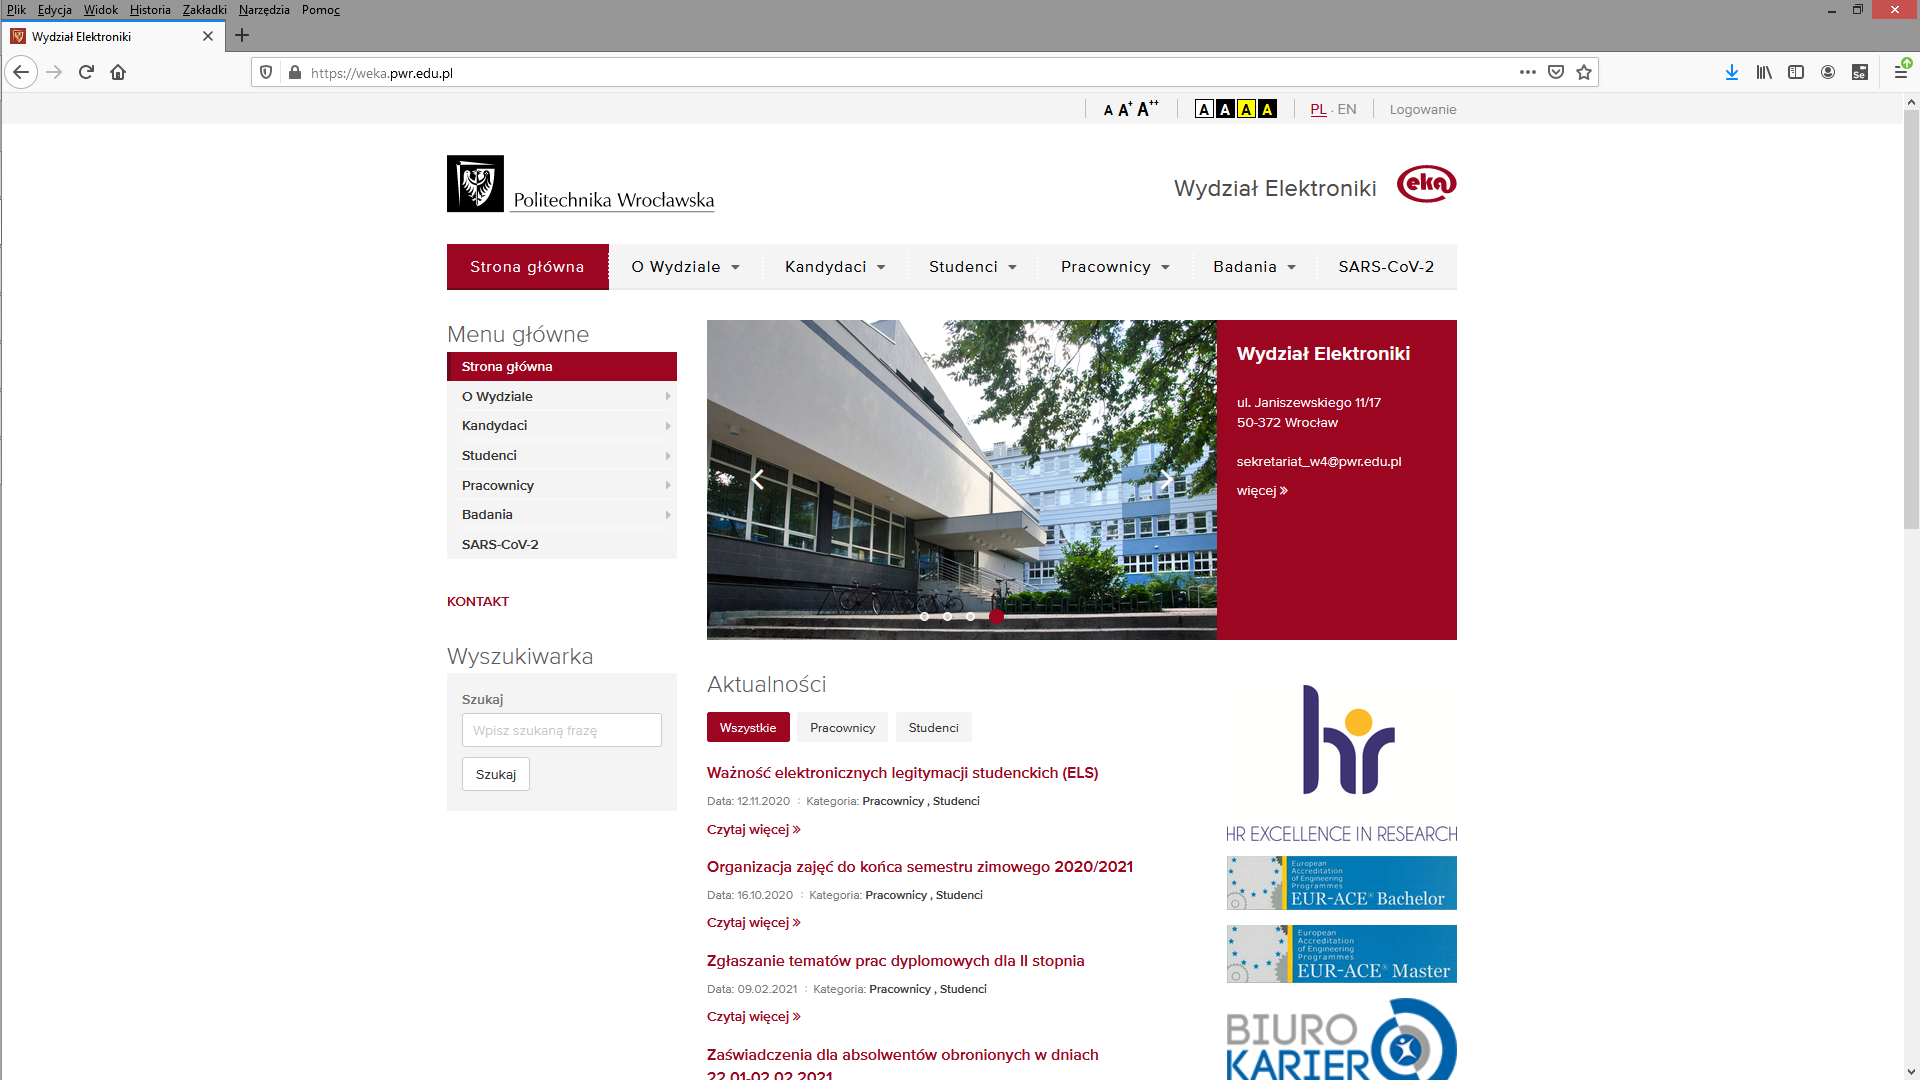
\includegraphics[width=0.475\textwidth]{rys05/zrzut1}}} & 
% 	\vtop{\vskip-2ex\hbox{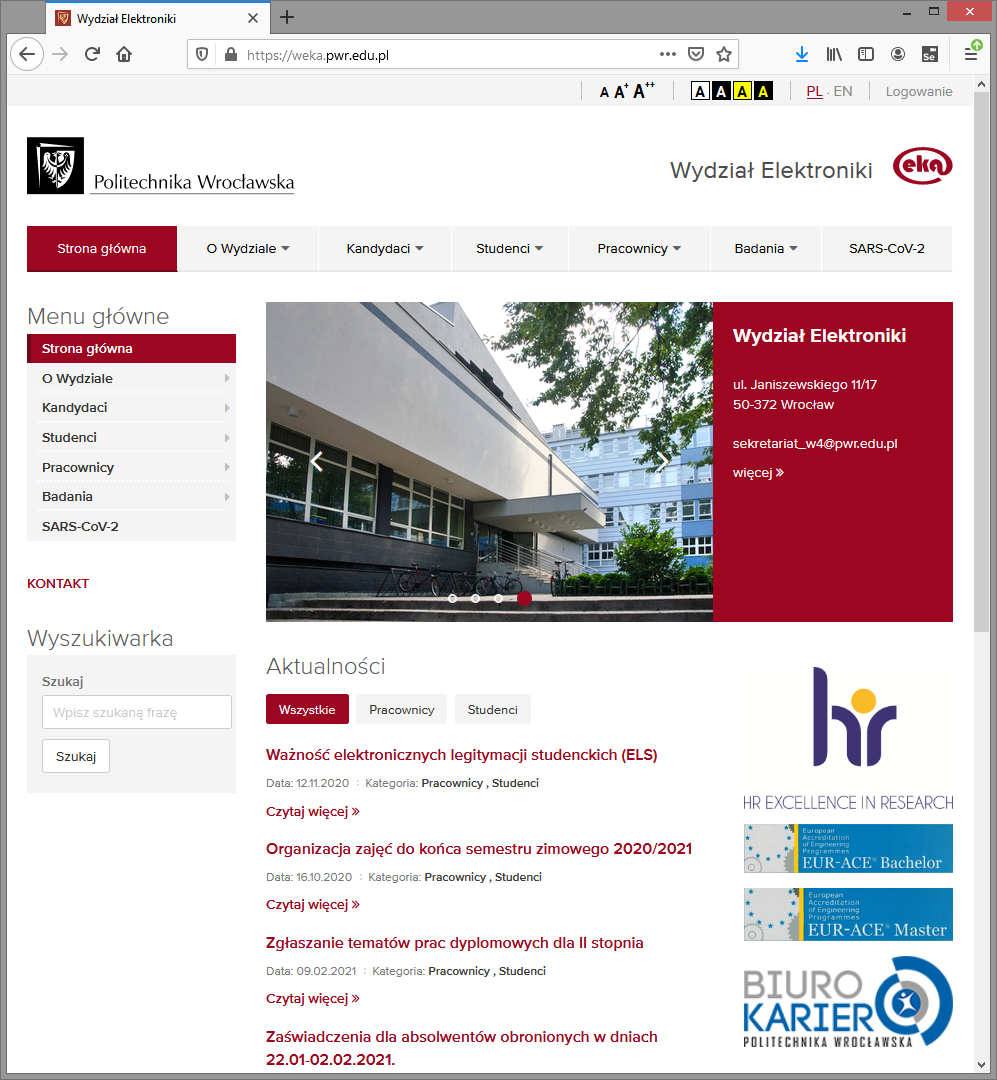
\includegraphics[width=0.475\textwidth]{rys05/zrzut2}}}
% 	% jeśli obraki są różnej wysokości, można je wyrównać do góry stosując vtop jak niżej
% 	% \vtop{\vskip-2ex\hbox{{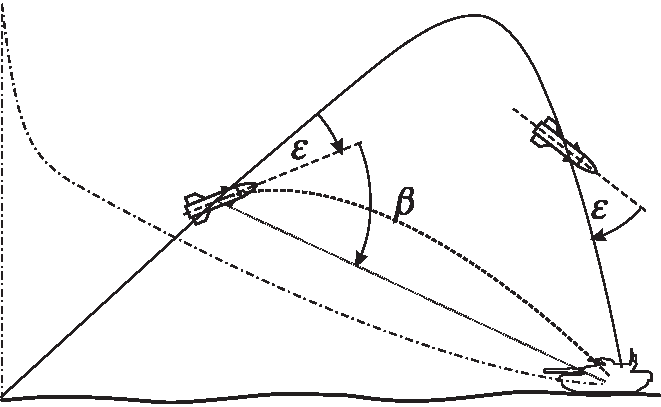
\includegraphics[width=0.475\textwidth]{rys05/beta1}}}} &
% 	% \vtop{\vskip-2ex\hbox{{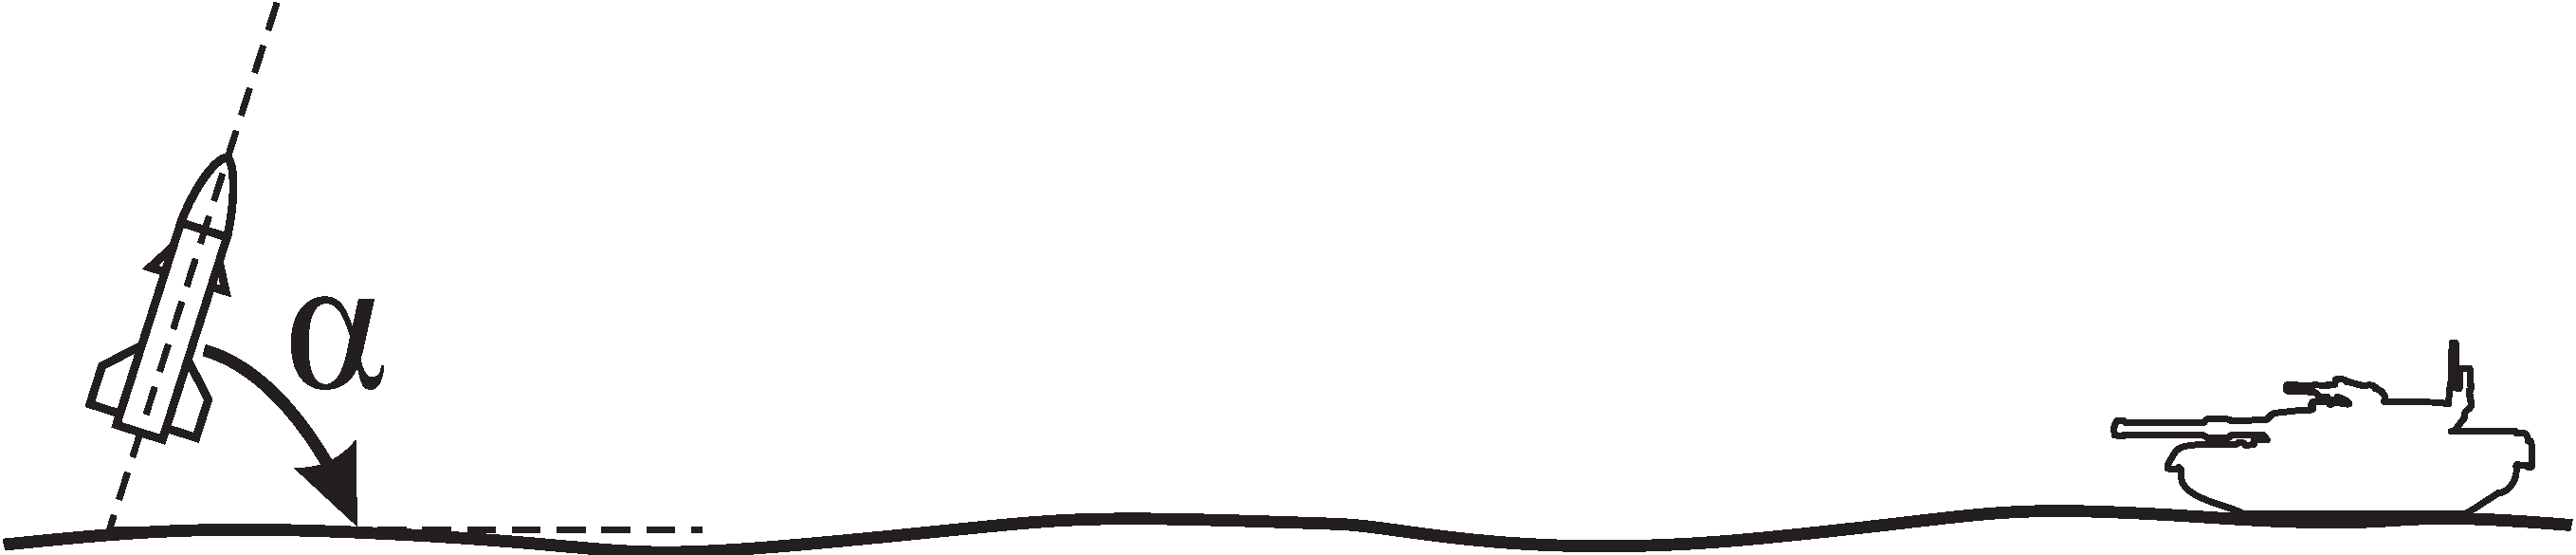
\includegraphics[width=0.475\textwidth]{rys05/alfa1}}}}  \caption{Wyznaczanie trajektorii lotu rakiety: 
% 	\end{tabular}
%   \caption{Przykłady zrzutów z ekranu: a) zły (nieczytelny, zrobiony przy zbyt szerokim oknie, z niepotrzebnymi marginesami, niepotrzebnym paskiem menu), b) w miarę dobry (w miarę czytelny, zrobiony przy zawężonym oknie, byłoby wskazane jeszcze usunięcie z niego beleczki z faviconem (jeśli nic nie wnosi) oraz przycięcie od dołu (jeśli treści tam pokazywane nie są istotne))}
%   \label{fig:zrzuty}
% \end{figure}

% 	
% Czasem problemem jest tworzenie zrzutów z ekranu, gdy występują na nim dane wrażliwe. Istnieją dwa sposoby na radzenie sobie z tym problemem.
% Pierwszy polega na zastąpieniu w~systemie danych danych rzeczywistych danymi testowymi -- wygenerowanymi tylko do celów prezentacji.
% Zrzut robi się wtedy na bazie danych testowych.
% Drugi polega na wykonaniu zrzutu z~ekranu, na którym pokazano dane rzeczywiste, i następnie zamianie tych danych już w pliku graficznym
% za pomocą odpowiedniego edytora (np.~\texttt{gimp}). Czyli oryginalny zrzut z ekranu należy otworzyć w edytorze, a potem
% nadpisać oryginalny tekst własnym tekstem. Konieczne jest wtedy dobranie odpowiednich czcionek aby nie było widać
% wprowadzonych zmian. 
% \begin{quotation}
% Uwaga: takie manipulowanie zrzutami jest usprawiedliwione jedynie w przypadku konieczności ochrony danych wrażliwych czy też lepszego pokazania wybranych elementów. Nie może to prowadzić generowania fałszywych rezultatów!!!
% \end{quotation}

% \section{Wstawianie kodu źródłowego}
% Kod źródłowy można wstawiać jako blok tekstu pisany czcionką maszynową. Używa się do tego otoczenie \verb?\lstlisting?. W atrybutach otoczenia można zdefiniować tekst podpisu wstawianego wraz z numerem nad blokiem, etykietę do tworzenia odwołań, sposób formatowania i~inne ustawienia. Zaleca się stosowanie w tym otoczeniu następujących parametrów:
% \begin{lstlisting}[basicstyle=\footnotesize\ttfamily]
% \begin{lstlisting}[label=list:req1,caption=Initial HTTP Request,
%                    basicstyle=\footnotesize\ttfamily]
% \end{lstlisting}
% Szczególnie przydatne podczas wstawiania większej ilości kodu źródłowego jest zastosowanie parametru \verb+basicstyle=\footnotesize\ttfamily+. Dzięki niemu zmniejsza się czcionka, a~przez to na stronie można zmieścić dłuższe linijki kodu. Użycie tak zdefiniowanego parametru nie jest jednak sztywnym zaleceniem. Wielkość czcionki można dobierać do potrzeb. 
% {\belowcaptionskip=-10pt
% \begin{lstlisting}[label=list:req1,caption=Initial HTTP Request,
%                    basicstyle=\footnotesize\ttfamily]
% GET /script/Articles/Latest.aspx HTTP/1.1
% Host: www.codeproject.com
% Connection: keep-alive
% Cache-Control: max-age=0
% Accept: text/html,application/xhtml+xml,application/xml
% User-Agent: Mozilla/5.0 ...
% Accept-Encoding: gzip,deflate,sdch
% Accept-Language: en-US...
% Accept-Charset: windows-1251,utf-8...
% \end{lstlisting}
% }
% Można też sformatować kod bez stosowania numerowanego podpisu (wtedy nie zamieszcza się \texttt{caption} na liście atrybutów).
% \begin{lstlisting}[basicstyle=\footnotesize\ttfamily]
% GET /script/Articles/Latest.aspx HTTP/1.1
% Host: www.codeproject.com
% Connection: keep-alive
% Cache-Control: max-age=0
% Accept: text/html,application/xhtml+xml,application/xml
% User-Agent: Mozilla/5.0 ...
% Accept-Encoding: gzip,deflate,sdch
% Accept-Language: en-US...
% Accept-Charset: windows-1251,utf-8...
% \end{lstlisting}

% Ponadto istnieje kilka sposobów wstawiania kodu źródłowego w bieżącej linijce tekstu:
% \begin{itemize} 
% \item korzystając z polecenia \verb?\texttt? ustawiającego czcionkę maszynową, jak w przykładzie \texttt{tutaj} (efekt zastosowania komendy \verb?\texttt{tutaj}?). Problemem jednak mogą okazać się znaki podkreślenia i inne znaki kontrolne.
% \item korzystają z otoczenia \verb?\verb? zapewniającego wypisanie kodu czcionką maszynową jak w~przykładzie \verb|tutaj| (efekt zastosowania komendy \verb?\verb|tutaj|?). Problemem jest to, że polecenie \verb?\verb? nie potrafi łamać dłuższego tekstu.
% \item korzystając z polecenia \verb?\lstin? umożliwiającego wypisanie kodu czcionką ustawianą w~opcjach jak w przykładzie
% \lstset{basicstyle=\ttfamily}\lstinline{tutaj} (efekt komendy \verb+\lstset{basicstyle=\ttfamily}\lstinline{tutaj}+) lub \lstinline[basicstyle=\ttfamily]=tutaj= (efekt komendy \verb+\lstinline[basicstyle=\ttfamily]=tutaj=+).
% \end{itemize}

% Poniżej zamieszczono przykłady kodów źródłowych z podświetleniem składni.

% \begin{lstlisting}[language=Java,style=JavaStyle,caption=Opis 1, label=lst:pierwszy]
% package pl.mrbarozoit.backend;

% import org.springframework.boot.SpringApplication;
% import org.springframework.boot.autoconfigure.SpringBootApplication;

% @SpringBootApplication
% public class BackendApplication {

%     public static void main(String[] args) {
%         SpringApplication.run(BackendApplication.class, args);
%     }

% }
% \end{lstlisting}

% Jeśli w kodzie źródłowym jest jakiś nieistotny fragment względem omawianego problemu, to można go wykropkować (patrz listing~\ref{lst:drugi}).

% {\belowcaptionskip=-9pt % To polecenie zmniejszy odległość podpisu od pokazywanego kodu (jego stosowanie jest zalecane)
% \begin{lstlisting}[language=JavaScript,style=JavaScriptStyle,caption=Opis 2, label=lst:drugi]
% // Karma configuration file, see link for more information
% // https://karma-runner.github.io/1.0/config/configuration-file.html

% module.exports = function (config) {
%   config.set({
%     basePath: '',
%     frameworks: ['jasmine', '@angular-devkit/build-angular'],
%     plugins: [
%       require('karma-jasmine'),
%       require('karma-chrome-launcher'),
%       require('karma-jasmine-html-reporter'),
%       require('karma-coverage-istanbul-reporter'),
%       require('@angular-devkit/build-angular/plugins/karma')
%     ],
%     ... // opuszczony kod
%     autoWatch: true,
%     browsers: ['Chrome'],
%     singleRun: false,
%     restartOnFileChange: true
%   });
% };
% \end{lstlisting}
% }

% Jeśli kod jest wąski, to można sformatować go w dwóch kolumnach jak na listingu~\ref{lst:kontrakt-board-move-in}.

% % Trzeba zacząć po linijce przerwy
% \begingroup 
% \listingcaption{Kontrakt na model wejściowy endpointu \texttt{/api/v1/chess/board/move}}
% \setlength\multicolsep{0pt plus 2pt}%
% \begin{lstlisting}[style=json-style, multicols=2, label=lst:kontrakt-board-move-in]
% {
%    "lastPosition": {
%       "fenDescription": "string"
%    },
%    "image": {
%       ...
%    },
%    "positions": {
%       "chessboardCorners": [
%          ...
%       ],
%       "tilesCornerPoints": [
%          ...
%       ]
%    },
%    "referenceColors": {
%       ...
%    },
% }
% \end{lstlisting}
% \vspace{6pt plus 2pt}
% \endgroup

% \section{Wykaz literatury oraz cytowania}
% \label{sec:literatura}
% Cytowania powinny być zamieszczane w tekście z użyciem komendy \verb+\cite{}+. Jej argumentem powinien być klucz cytowanej pozycji (lub lista kluczy  rozdzielonych przecinkiem bez spacji, jeśli takich pozycji w danym miejscu cytuje się więcej) jaki jest używany w bazie danych bibliograficznych (plik \texttt{dokumentacja.bib}). Po kompilacji \texttt{bibtex} i \texttt{pdflatex} w tekście pojawia się właściwy odsyłacz do pozycji w wykazie literatury (ujęty w kwadratowe nawiasy -- zgodnie z~tym, co definiuje styl \texttt{plabbrv.bst}), zaś w samym wykazie (rozdział Literatura) -- zacytowana pozycja. Przykładem cytowania jest: ,,dobrze to opisano w pracach~\cite{JS07,SQL2}'' (gdzie zastosowano komendę \verb?\cite{JS07,SQL2}?).

% Co do zawartości rekordów bibliograficznych - style bibtexowe potrafią ,,skracać'' imiona (czyli wstawiać, jeśli taka wola, inicjały zamiast pełnych imion). Niemniej dobrze jest od razu przyjąć jakąś konwencję. Proponuje się, aby w rekordach od razu wstawiane były inicjały zamiast pełnych imion.

% Niekiedy tytuły prac zawierają wyrazy z dużymi i małymi literami. Takie tytuły należy brać w podwójne nawiasy klamrowe, aby \texttt{bibtex} nie zamienił ich na postać, w której poza pierwszą literą pozostałe są małe.

% Jeśli jakiś cytowany zasób pochodzi z Internetu, to jego rekord w pliku \texttt{bib} powinien wyglądać jak niżej.
% \begin{lstlisting}[basicstyle=\footnotesize\ttfamily]
% @INPROCEEDINGS{SQL2, 
%   title={{A MySQL-based data archiver: preliminary results}}, 
%   author={Bickley, M. and Slominski, Ch.},
%   booktitle = {{Proceedings of ICALEPCS07}},
% 	month = oct,
% 	day = {15--19},
% 	year={2007}, 
%   note={\url{http://www.osti.gov/scitech/servlets/purl/922267} 
% 	[dostęp dnia 20 czerwca 2015]}
% }
% \end{lstlisting}
% A to inny przykład rekordu danych bibliograficznych:
% \begin{lstlisting}[basicstyle=\footnotesize\ttfamily]
% @TechReport{JS07,
% 	author = {Jędrzejczyk, J. and Śródka, B.},
% 	title  ={Segmentacja obrazów metodą drzew decyzyjnych},
% 	year = {2007},
% 	institution = {Politechnika Wrocławska, Wydział Elektroniki}
% }
% \end{lstlisting}

% \section{Indeks rzeczowy}
% \label{sec:indeks}
% Generowanie indeksu \index{generowanie!-- indeksu} po trosze wygląda jak generowanie wykazu literatury \index{generowanie!-- wykazu literatury}-- wymaga kilku kroków. Podczas pierwszej kompilacji \texttt{pdflatex} generowany jest plik z rozszerzeniem \texttt{*.idx} (zawierający ,,surowy indeks''). Następnie, bazując na tym pliku, generowany jest plik z rozszerzeniem \texttt{*.ind} zawierający sformatowane dane. Ten krok wymaga uruchomienia odpowiedniego narzędzia oraz zastosowania plik z definicją stylu \texttt{Dyplom.ist}. W kroku ostatnim dokonuje się kolejnej kompilacji \texttt{pdflatex} (dzięki niej w wynikowym dokumencie pojawi się Indeks rzeczowy). Domyślnie Indeks rzeczowy zostanie sformatowany w~układzie dwukolumnowym.

% Oczywiście aby to wszystko zadziałało w kodzie szablonu należy umieścić odpowiednie komendy definiujące elementy indeksu rzeczowego (\verb?\index?) oraz wstawiające sformatowany Indeks rzeczowy do dokumentu wynikowego (\verb?\printindex?). Więcej informacji o tworzeniu indeksu rzeczowego można znaleźć na stronie \url{https://en.wikibooks.org/wiki/LaTeX/Indexing}. Poniżej przedstawiono przykłady komend użytych w szablonie do zdefiniowania elementów indeksu rzeczowego:
% \begin{itemize}
% \item \verb?\index{linia komend}? -- pozycji główna.
% \item \verb?\index{generowanie!-- indeksu}? -- podpozycja.
% \end{itemize}

% Generowanie pliku \texttt{*.ind} można inicjować na kilka sposobów:
% \begin{itemize}
% \item poprzez wydanie odpowiedniego polecenia bezpośrednio w linii komend \index{linia komend}
% \begin{lstlisting}[basicstyle=\footnotesize\ttfamily]
% makeindex Dyplom.idx -t Dyplom.ilg -o Dyplom.ind -s Dyplom.ist
% \end{lstlisting}
% \item poprzez odpalenie odpowiedniego narzędzia środowiska. Na przykład w \texttt{TeXnicCenter} definiuje się tzw. \texttt{output profiles}: 
% \begin{lstlisting}[basicstyle=\footnotesize\ttfamily]
% makeindex "%tm.idx" -t "%tm.ilg" -o "%tm.ind" -s "%tm.ist"
% \end{lstlisting}
% a samo generowanie pliku \texttt{*.ind} zapewni wybranie pozycji menu \texttt{Build/Makeindex}.
% \item korzystając z odpowiednio sparametryzowanych pakietów i komend wewnątrz kompilowanego dokumentu (czyli od razu przy okazji jego kompilacji).
% \begin{lstlisting}[basicstyle=\footnotesize\ttfamily]
% \DisemulatePackage{imakeidx}
% \usepackage[noautomatic]{imakeidx} 
% % jeśli chcemy, by indeks by generowany automatycznie programem makeindex:
% %\usepackage[makeindex]{imakeidx} 
% % a tak ponoć można przekazać opcje do programu generującego indeks:
% %\makeindex[options=-s podrecznik -L polish -M lang/polish/utf8] 
% %\makeindex[options=-s podrecznik]
% \makeindex
% \end{lstlisting}

% Niestety, \texttt{makeindex} jest narzędziem, które umieszcza część pozycji w grupie \texttt{Symbols}, a~nie w grupach związanych z literkami alfabetu. W związku z czym indeksowany element zaczynający się od polskiej literki trafia do grupy \texttt{Symbols}, jak np.~\verb?\index{Światło}?\index{Światło}. Jeśli chce się zamieszczać w indeksie symbole matematyczne, to dobrze jest to robić jak w następującym przykładzie: \verb?\index{$asterisk@$\ast$}? \index{$asterisk@$\ast$} czy też \verb?\index{c@$\mathcal{C}$}?\index{c@$\mathcal{C}$}, tj.~dostarczając przy okazji klucz do sortowania.
% Lepiej w tym względzie radzą sobie inne narzędzia, jak \texttt{texindy} lub \texttt{xindy} dostępne pod linuxem. Korzystając z nich uzyskuje się grupy polskich literek w indeksie rzeczowym (hasła zaczynające się od polskich literek już nie trafiają do grupy Symbols). Przykład polecenia wydanego z linii komend, w którym wykorzystano \texttt{texindy} zamieszczono poniżej (zakładamy kodowanie plików w UTF8, można dla niniejszego szablonu zmienić na cp1250):
% \begin{lstlisting}[basicstyle=\footnotesize\ttfamily]
% texindy -L polish -M lang/polish/utf8 Dyplom.idx
% \end{lstlisting}

% To polecenie wygeneruje \texttt{Dyplom.ind} o zawartości:
% \begin{lstlisting}[basicstyle=\footnotesize\ttfamily]
% \begin{theindex}
%   \providecommand*\lettergroupDefault[1]{}
%   \providecommand*\lettergroup[1]{%
%       \par\textbf{#1}\par
%       \nopagebreak
%   }

%   \lettergroup{G}
%   \item generowanie
%     \subitem -- indeksu, 27
%     \subitem -- wykazu literatury, 27

%   \indexspace

%   \lettergroup{L}
%   \item linia komend, 27

%   \indexspace

%   \lettergroup{Ś}
%   \item \'Swiat\IeC {\l }o, 28

% \end{theindex}
% \end{lstlisting}


% \end{itemize}


% Aby mieć większą kontrolę automatyczne generowanie indeksu zostało w niniejszym szablonie wyłączone (indeks trzeba wygenerować samemu, wydając polecenie \texttt{makeindex} lub zalecane \texttt{texindy}).

% \section{Inne uwagi}
% Dobrym sposobem na kontrolę błędów występujących podczas kompilacji jest wstawianie linijki \verb?\end{document}? w wybranym miejscu dokumentu. Jest to szczególnie przydatne w przypadkach, gdy błędy te są trudne do zidentyfikowania (gdy wygenerowane przez kompilator numery linii z błędami nie są tymi, w których błędy występują). Wystarczy wtedy przestawić wspomnianą linijkę do kolejnych miejsc, aż znajduję to miejsce, gdzie występuje problem.

% Aby osiągnąć apostrofy maszynowe (złożone z samych kresek) należy użyć polecenia \verb?"{}jak tutaj{}"? (podwójny apostrof stojący bezpośrednio przed niektórymi literkami zamienia je na literki z akcentami, aby temu zapobiec dostawiono nawiasy klamrowe). W efekcie otrzymamy "{}jak tutaj{}". Jeśli natomiast apostrofy mają być drukarskie (złożone z kropek i kresek), to należy użyć polecenia \verb?,,jak tutaj''? (dwa pojedyncze przecinki i dwa pojedyncze apostrofy). W efekcie otrzymamy ,,jak tutaj''. Można też użyć znaków apostrofów odpowiednio zakodowanych „jak tutaj”, tylko że czasem trudno pisze się takie apostrofy w środowiskach kompilacji projektów latexowych.


% Oto sposoby ustawienia odstępów między liniami:
% \begin{itemize}
% \item używając komendy \verb+\linespread{...}+ (akceptowalne), przy czym atrybutem tej metody jest współczynnik zależny od wielkości
% czcionki.  Dla czcionki wiodącej 12pt odstęp półtora linii osiągnie się komendą \verb+\linespread{1.241}+. Dla innych czcionek wiodących wartości tego parametru są jak w poniższym zestawieniu.
% \begin{lstlisting}[basicstyle=\footnotesize\ttfamily]
% 10pt 1.25 dla \onehalfspacing 
%      1.667 for \doublespacing, 
% 		 ponieważ ,,basic ratio'' = 1.2 
% 		(\normalfont posiada \baselineskip rozmiaru 12pt)
% 11pt 1.213 dla \onehalfspacing oraz 1.618 dla \doublespacing, 
%      ponieważ ,,basic ratio'' = 1.236 
% 		(\normalfont posiada \baselineskip rozmiaru 13.6pt)
% 12pt 1.241 dla \onehalfspacing oraz 1.655 dla \doublespacing, 
%      ponieważsince ''basic ratio'' is 1.208 
% 		(\normalfont has a \baselineskip of 14.5pt)
% \end{lstlisting}
% Kłopot w tym, że raz ustawiony odstęp będzie obowiązywał do wszystkich czcionek (brak jest mechanizmu zmiany współczynnika w zależności od wielkości czcionki akapitu).

% \item używając pakietu \texttt{setspace} (niezalecane). Ponieważ klasa \texttt{memoir} emuluje pakiet \texttt{setspace}, w preambule dokumentu należałoby umieścić:
% \begin{lstlisting}[basicstyle=\footnotesize\ttfamily]
% \DisemulatePackage{setspace}
% \usepackage{setspace}
% \end{lstlisting}
% a potem można już sterować odstęp komendami:
% \begin{lstlisting}[basicstyle=\footnotesize\ttfamily]
% \singlespacing
% \onehalfspacing
% \doubelspacing
% \end{lstlisting}
% Ten sposób pozwala na korzystanie z mechanizmu automatycznej zmiany odległości linii w~zależności od wielkości czcionki danego akapitu.
% \item korzystając bezpośrednio z komend dostarczonych w klasie \texttt{memoir} (zalecane):
% \begin{lstlisting}[basicstyle=\footnotesize\ttfamily]
% \SingleSpacing
% \OnehalfSpacing
% \DoubleSpacing
% \end{lstlisting}
% Ten sposób również pozwala na korzystanie z mechanizmu automatycznej zmiany odległości linii w zależności od wielkości czcionki danego akapitu.
% \end{itemize}

% Na koniec jeszcze uwaga o rozmiarze pliku wynikowego. Otóż \texttt{pdflatex} generuje pliki \texttt{pdf}, które zazwyczaj mogłyby być nieco lepiej
% skompresowane. Do lepszego skompresowania tych plików można użyć programu \texttt{ghostscript}. Wystarczy w tym celu wydać komendę (pod windowsami):
% \begin{lstlisting}[basicstyle=\footnotesize\ttfamily]
% gswin64 -sDEVICE=pdfwrite -dCompatibilityLevel=1.4 -dNOPAUSE -dQUIET \
% -dSAFER -dBATCH -sOutputFile=Dyplom-compressed.pdf Dyplom.pdf
% \end{lstlisting}
% W poleceniu tym można również wstawić opcję \texttt{-dPDFSETTINGS=/prepress} (zapewniającą uzyskanie wysokiej jakości, zachowanie kolorów, uzyskanie obrazków w rozdzielczości 300 dpi). Ze względów licencyjnych ghostscript używa domyślnie algorytmów z kompresją stratną. Przy kompresji może więc dojść do utraty jakości bitmap.

\chapter{Badania symulacyjne}\label{chap:research}


% \section{Porównanie wyników optymalizacji z literaturą~\cite{evolutionary_puredata}}

Praca wykorzystuje próbki dźwięku z literatury~\cite{evolutionary_puredata_results}
aby przetestować zaimplementowany algorytm i jednocześnie porównać jego wyniki
z podobną pracą. Wykorzystano te próbki dźwięku
z literatury, które \textbf{nie zostały wygenerowane} za pomocą
oprogramowania do syntezy \textit{Pure Data}~\cite{pure_data},
ponieważ oryginalna praca wykorzystywała
to oprogramowanie jako środowisko do syntezy dźwięku -- takie porównanie
nie byłoby miarodajne, ponieważ algorytm z literatury miałby do dyspozycji
dokładnie takie same algorytmy, które zostały wykorzystane do wygenerowania
dźwięków docelowych.
Przed przeprowadzeniem optymalizacji ustalono wartość częstotliwości podstawowej~$f_0$
dla każdego z testowanych dźwięków, aby algorytm optymalizował parametry kontrolujące
jedynie barwę dźwięku dla z góry zadanej właściwej wysokości dźwięku.
Podobną praktykę stosują badania z literatury~\cite{ieee_synth_programming}.
Zastosowano implementację algorytmu estymującego częstotliwość podstawową
\textit{YIN}~\cite{yin_pitch_estimation}, dostępną w pakiecie obliczeniowym
\texttt{librosa}~\cite{librosa}. Przebieg procesu optymalizacji dla każdego z testowanych
dźwięków umieszczony jest na płycie CD, co opisuje dodatek~\ref{chap:opis-plyty}.

\subsubsection{Parametry algorytmu genetycznego}

W badaniach zastosowano następujące parametry algorytmu genetycznego:

\begin{enumerate}
  \item rozmiar populacji: \texttt{50},
  \item liczba iteracji: \texttt{200},
  \item strategia mutacji: \texttt{best1bin},
  \item rekombinacja: \texttt{0.7}.
\end{enumerate}

Ze względu na długi czas działania zaimplementowanego algorytmu optymalizacji
(średnio 10 minut na pojedynczą iterację),
w pracy nie udało się porównać jak różne parametry algorytmu genetycznego
wpływają na proces optymalizacji. Finalnie wykonano tylko jedną pełną optymalizację
dla każdego z testowanych dźwięków.

\newpage

\section{Dźwięk fletu}

Dźwięk \texttt{flute.wav}~(rysunek~\ref{fig:literature_flute_sound_overview})
jest nagraniem prawdziwego instrumentu dętego. Kształt fali jest nieregularny,
charakterystyka spektralna zawiera dynamicznie pojawiające się i słabnące 
składowe częstotliwościowe.

% \begin{multicols}{3}
\begin{figure}[H]
    \centering
    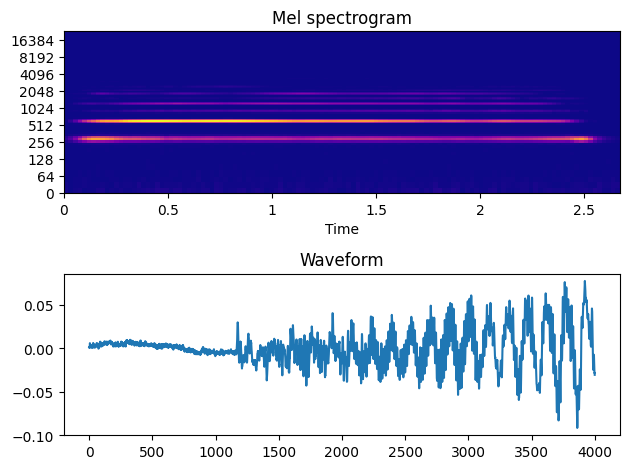
\includegraphics[width=0.7\linewidth]{rys06/target_sample_flute_literature.png}
    \caption{
      Spektrogram i wykres fali dla dźwięku \texttt{flute.wav} wykorzystywanego
      do eksperymentów w~\cite{evolutionary_puredata_results}.
    }\label{fig:literature_flute_sound_overview}
\end{figure}

\begin{figure}[H]
    \centering
    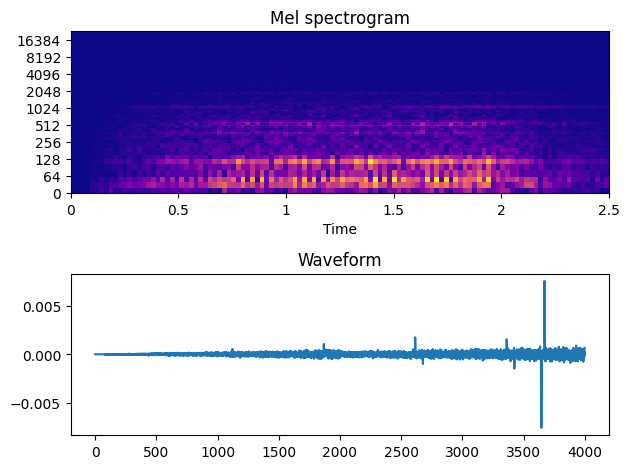
\includegraphics[width=0.7\linewidth]{rys06/evolved_sample_flute.png}
    \caption{
      Spektrogram i wykres fali dla dźwięku \texttt{flute.wav}
      wytworzonego przez zaimplementowany algorytm optymalizacji
      dla dźwięku \texttt{flute.wav}.
    }\label{fig:evolved_flute_sound_overview}
\end{figure}

\begin{figure}[H]
    \centering
    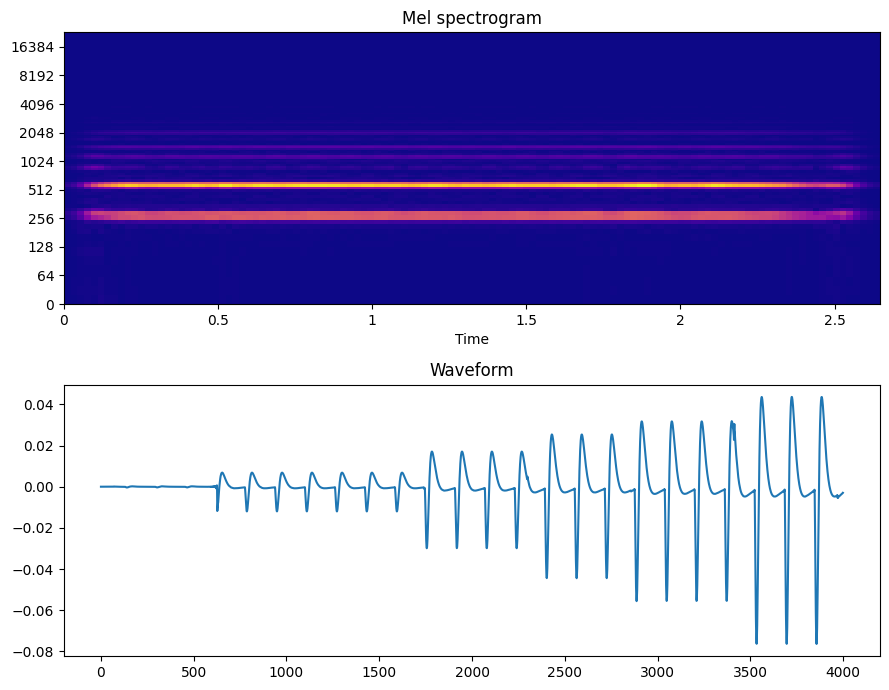
\includegraphics[width=0.7\linewidth]{rys06/macret_evolved_flute.png}
    \caption{
      Spektrogram i wykres fali dla dźwięku
      wygenerowanego przez algorym z literatury~\cite{evolutionary_puredata}
      na wzór \texttt{flute.wav}.
    }\label{fig:evolved_literature_flute}
\end{figure}
% \end{multicols}

\begin{figure}[H]
    \centering
    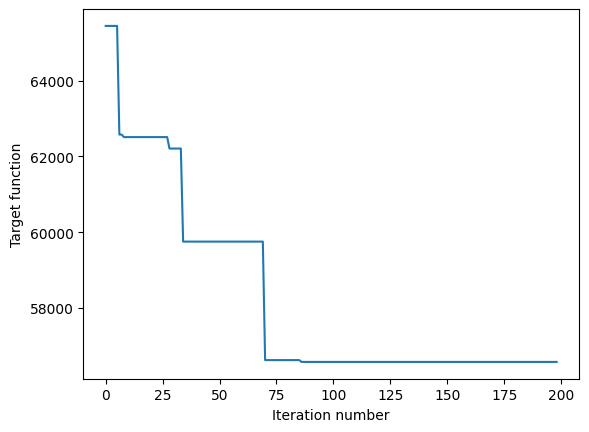
\includegraphics[width=0.6\linewidth]{rys06/flute_target_fun_values.png}
    \caption{
      Zmiany wartości funkcji celu podczas optymalizacji.
    }%\label{fig:evolved_literature_flute}
\end{figure}



\section{Sampel z syntezatora \textit{OP-1}}

Dźwięk \texttt{op1\_1.wav}, wygenerowany przy pomocy syntezatora \textit{OP-1} jest próbą
zasymulowania dźwięku instrumentu dętego przez syntezator. Podobnie jak w przypadku
prawdziwego dźwięku fletu, widoczne są zmienne w czasie składowe harmoniczne, jednak
sygnał wygenerowany na syntezatorze jest bardziej stabilny.

% \begin{multicols}{3}
\begin{figure}[H]
    \centering
    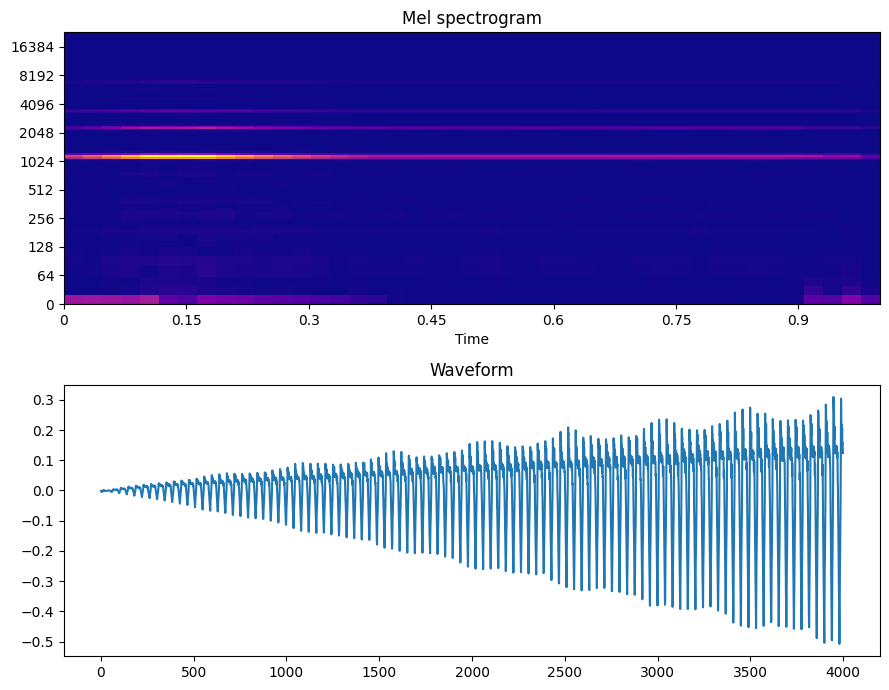
\includegraphics[width=0.7\linewidth]{rys06/target_sample_op1_literature.png}
    \caption{
      Spektrogram i wykres fali dla dźwięku \texttt{op1\_1.wav} wykorzystywanego
      do eksperymentów w~\cite{evolutionary_puredata_results}.
    }\label{fig:literature_op_1_sound_overview}
\end{figure}


\begin{figure}[H]
    \centering
    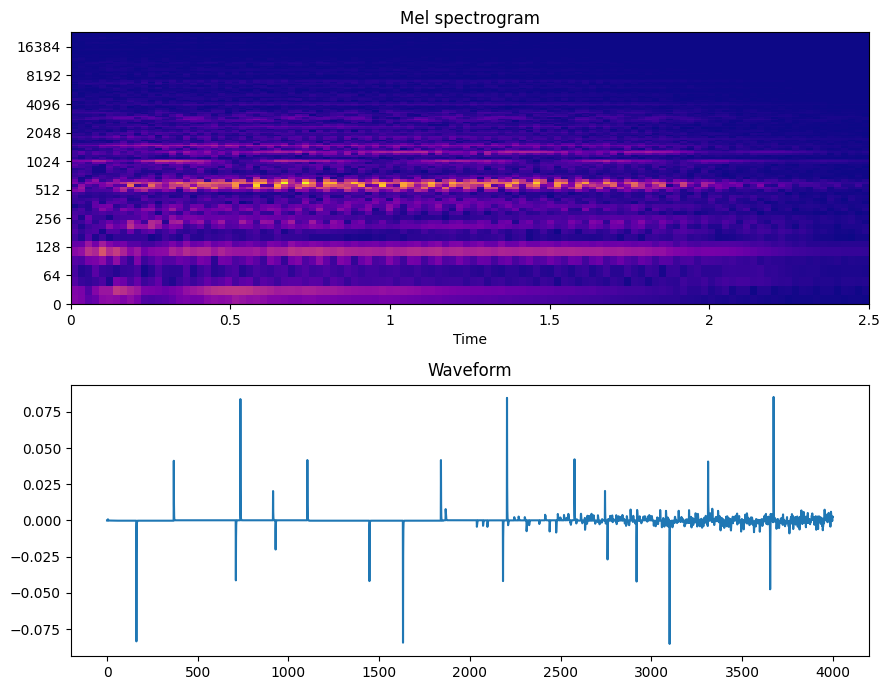
\includegraphics[width=0.7\linewidth]{rys06/evolved_sample_op1.png}
    \caption{
      Spektrogram i wykres fali dla dźwięku wygenerowanego
      przez algorytm optymalizacji na wzór \texttt{op1\_1.wav}.
    }\label{fig:evolved_op1_sound_overview}
\end{figure}


\begin{figure}[H]
    \centering
    \includegraphics[width=0.7\linewidth]{rys06/macret_evolved_op1.png}
    \caption{
      Spektrogram i wykres fali dla dźwięku wygenerowanego
      przez algorytm z literatury~\cite{evolutionary_puredata} na wzór \texttt{op1\_1.wav}.
    }\label{fig:evolved_literature_op1_sound_overview}
\end{figure}
% \end{multicols}

\begin{figure}
    \centering
    \includegraphics[angle=90,width=0.45\linewidth]{rys06/evolved_graph_op1.png}
    \caption{
      Graf DSP wygenerowany przez zaimplementowany algorytm
      dla dźwięku docelowego \texttt{op1\_1.wav}.
    }\label{fig:evolved_graph_op1}
\end{figure}


\begin{figure}[H]
    \centering
    \includegraphics[width=0.6\linewidth]{rys06/op1_target_fun_values.png}
    \caption{
      Zmiany wartości funkcji celu podczas optymalizacji.
    }%\label{fig:evolved_literature_flute}
\end{figure}

\section{Transjent}

Dźwięk \texttt{transient.wav}, przedstawiony na rysunku~\ref{fig:literature_transient_sound_overview},
został wykorzystany w literaturze~\cite{evolutionary_puredata} do sprawdzenia jak dobrze algorytm
generujący dźwięk potrafi przybliżyć dźwięki o dynamicznych zmianach w charakterystyce spektralnej.
Tego typu dźwięki przypominają brzmienie instrumentów klawiszowych: fortepianu lub klawesynu.

% \begin{multicols}{3}
\begin{figure}[H]
    \centering
    \includegraphics[width=0.7\linewidth]{rys06/transient_sample_literature.png}
    \caption{
      Spektrogram i wykres fali dla dźwięku \texttt{transient.wav} wykorzystywanego
      do eksperymentów w~\cite{evolutionary_puredata_results}.
    }\label{fig:literature_transient_sound_overview}
\end{figure}

\begin{figure}[H]
    \centering
    \includegraphics[width=0.7\linewidth]{rys06/evolved_sample_transient.png}
    \caption{
      Spektrogram i wykres fali dla dźwięku wygenerowanego na wzór
      \texttt{transient.wav}.
    }\label{fig:evolved_transient_sound_overview}.
\end{figure}

\begin{figure}[H]
    \centering
    \includegraphics[width=0.7\linewidth]{rys06/macret_evolved_transient.png}
    \caption{
      Spektrogram i wykres fali dla dźwięku wygenerowanego 
      przez algorytm z literatury~\cite{evolutionary_puredata} na wzór
      \texttt{transient.wav}.
    }\label{fig:evolved_literature_transient_sound_overview}.
\end{figure}
% \end{multicols}

\begin{figure}[H]
    \centering
    \includegraphics[width=0.6\linewidth]{rys06/transient_target_fun_values.png}
    \caption{
      Zmiany wartości funkcji celu podczas optymalizacji.
    }%\label{fig:evolved_literature_flute}
\end{figure}

\begin{figure}
    \centering
    \includegraphics[angle=90,width=0.35\linewidth]{rys06/evolved_graph_transient.png}
    \caption{
      Graf DSP wygenerowany przez zaimplementowany algorytm
      dla dźwięku docelowego \texttt{transient.wav}.
    }\label{fig:evolved_graph_transient}
\end{figure}



\section{Dźwięki inne niż przykłady z literatury}\label{sec:non_literature_samples}

Badania przeprowadzone w ramach~\cite{evolutionary_puredata}
wykorzystują ograniczony zbiór dźwięków, koncentrując
się na instrumentach dętych i syntezie FM\@. Algorytm przetestowano
również na samodzielnie wytworzonych dźwiękach, wykorzystując syntezę
subtraktywną~\ref{fig:minilogue_target_sample}.

% \begin{multicols}{2}
\begin{figure}[H]
    \centering
    \includegraphics[width=0.7\linewidth]{rys06/target_minilogue.png}
    \caption{
      Spektrogram i wykres fali dla dźwięku wygenerowanego 
      na syntezatorze \textit{Korg Minilogue xd}.
    }\label{fig:minilogue_target_sample}
\end{figure}

\begin{figure}[H]
    \centering
    \includegraphics[width=0.7\linewidth]{rys06/evolved_minilogue.png}
    \caption{
      Spektrogram i wykres fali dla dźwięku wygenerowanego 
      przez zaimplementowany w ramach pracy algorytm na
      wzór~\ref{fig:minilogue_target_sample}.
    }\label{fig:evolved_minilogue_sample}.
\end{figure}
% \end{multicols}


\begin{figure}
    \centering
    \includegraphics[angle=90,width=0.44\linewidth]{rys06/evolved_graph_minilogue.png}
    \caption{
      Graf DSP wygenerowany przez zaimplementowany algorytm
      dla dźwięku docelowego~\ref{fig:minilogue_target_sample}.
      Poprawnie został odtworzony filtr niskoprzepustowy oraz
      sterujący nim sygnał ADSR\@.
    }\label{fig:evolved_graph_op1}
\end{figure}


\chapter{Analiza wyników, możliwe drogi dalszych badań}\label{chap:results_analysis}


% Wyniki uzyskane przez zaimplementowany algorytm optymalizacji
% opisane w rozdziałach~\ref{chap:research} oraz~\ref{target_function_chapter} pozwalają

Wyniki przedstawione w rozdziałach~\ref{chap:research} oraz~\ref{target_function_chapter}
wskazują, że zaimplementowany algorytm optymalizacji wytwarza poprawne rozwiązania
dla części problemów. Nawet gdy finalnie wygenerowane brzmienie różni
się od dźwięku docelowego, algorytm wytwarza interesujące barwy dźwięku,
które można zakwalifikować jako~,,wariacje'' na temat oryginalnego sygnału.
Tego typu wyniki mogą być wartościowe dla potencjalnych użytkowników algorytmu.
W niniejszym rozdziale przeprowadzono szczegółową analizę obserwacji,
uzyskanych podczas procesu badawaczego.


\section{Zbiór danych testowych}\label{sec:not_enough_benchmarking_data}

Automatyczna konstrukcja elektronicznych instrumentów muzycznych jest stosunkowo
nowym obszarem badań, w związku z czym brakuje odpowiednich zbiorów danych
umożliwiających porównywanie sprawności różnych algorutmów.
Porównanie wykonane w niniejszej pracy nie stanowi przekroju
przez wiele możliwych typów syntezy, ponieważ w procesie przeglądu
literatury nie udało się znaleźć stosownego zbioru danych.

Jak pokazały wyniki opisane w sekcji~\ref{sec:non_literature_samples},
zaimplementowany algorytm generuje lepsze rozwiązania w przypadku
syntezy \textit{analog modeling}, podczas gdy praca służąca
za porównanie~\cite{evolutionary_puredata} zawiera głownie przykłady
syntezy FM oraz nagrania instrumentów dętych. Sugestie dotyczące
stworzenia bardziej różnorodnego zbioru dźwięków o różnych barwach
i dynamice zawarto w sekcji~\ref{sec:potential_improvements}.


\section{Optymalizacja parametrów grafu dla problemów o małej złożoności}

Jak wykazały testy przeprowadzone w rozdziale~\ref{target_function_chapter},
zaimplementowany algorytm jest w stanie dokładnie odtworzyć wartości
parametrów grafu dla prostych problemów syntezy
FM~(\ref{fig:param_optimisation_results_spectrograms})
i umiarkowanie złożonych problemów syntezy
\textit{analog modeling}~(\ref{fig:am_param_optimisation_results_spectrograms}).
Testy na małej próbie słuchaczy pozwalają stwierdzić,
że \textbf{nie są oni w stanie odróżnić} sygnałów wygenerowanych
dla problemów z rozdziału~\ref{target_function_chapter}
od dźwięków docelowych.

% \begin{enumerate}
%   \item Nawet jak nie działa to idzie w kierunku celu, często generując interesujące brzmienia po drodze,
%   \item Problemy ze zmianami w dynamice, szczególnie pierwsze ułamki sekund,
% \end{enumerate}


\section{Potencjał wykorzystania w przemyśle muzycznym}

Wytwarzane przez algorytm barwy są zróżnicowane i brzmią
w sposób~,,muzyczny'' -- nawet gdy wygenerowany dźwięk
znacząco różni się od docelowej barwy, algorytm nie generuje
szumu ani~,,kakofonii''. 
Zaimplementowany algorytm może być uruchomiony na standardowym komputerze,
dostępnym dla przeciętnego użytkownika, co otwiera możliwość jego integracji
z oprogramowaniem typu \textit{digital audio workstation}. Integracja
z oprogramowaniem do produkcji muzyki otwiera drogę do wykorzystania
wtyczek \texttt{VST}, znacznie zwiększając liczbę dostępnych
dla algorytmu węzłów przetwarzania sygnału, potencjalnie usprawniając
jego działanie.


\section{Potencjalne usprawnienia wydajności algorytmu}

\begin{figure}[H]
    \centering
    \includegraphics[width=1.0\linewidth]{rys07/profile_target_function_execution.png}
    \caption{
      Wizualizacja danych wygenerowanych przez profiler języka Python
      dla przykładowego problemu optymalizacji. Widoczne składowe wpływające
      na sumaryczny czas ewaluacji funkcji celu.
      Czerwoną strzałką oznaczono czas poświęcony
      na syntezę dźwięku w grafie DSP\@.
    }\label{fig:target_function_profiling}
\end{figure}

\begin{figure}[H]
    \centering
    \includegraphics[width=1.0\linewidth]{rys07/mfcc_search.png}
    \caption{
      Porównanie czasu obliczania współczynników MFCC (\texttt{dsp.py:115})
      oraz czasu działania algorytmu DTW (\texttt{dsp.py:171}).
    }\label{fig:mfcc_profiling}
\end{figure}

Rysunki~\ref{fig:target_function_profiling} oraz~\ref{fig:mfcc_profiling}
przedstawiają wyniki profilowania zaimplementowanego algorytmu, wykonane
za pomocą narzędzia \href{https://jiffyclub.github.io/snakeviz/}{\texttt{snakeviz}}.
W pracy została wykorzystana gotowa implementacja
algorytmu DTW (\textit{dynamic time warping}) w języku \texttt{Python}, której
wykonanie zajmuje największą część czasu obliczania wartości funkcji celu.
Wykorzystanie pakietu numerycznego \texttt{numpy} bądź implementacja DTW w
kompilowanym języku programowania może znacząco poprawić szybkość działania algorytmu.

\section{Potencjalne drogi dalszego rozwoju algorytmu}\label{sec:potential_improvements}

Pierwszym krokiem, który należy wykonać w celu usprawnienia
algorytmu optymalizacji jest przygotowanie zbioru dźwięków,
które będą służyły za \textbf{zbiór weryfikujący poprawność działania algorytmu}.
Przykłady zaczerpnięte z literatury~\cite{evolutionary_puredata_results}
nie zawierają wystarczająco bogatej gamy możliwych do wygenerowania
barw dźwięku, które wymusiłyby na algorytmie optymalizacji wykorzystanie
różnorodnych algorytmów syntezy i struktur grafu DSP\@. Wyniki
eksperymentów wykonanych w rozdziale~\ref{chap:research} pozwalają
na zasugerowanie zbioru cech dźwięków, których warianty
powinny być zawarte w zbiorze weryfikującym:

\begin{enumerate}
  \item Typ syntezy:
  \begin{itemize}
    \item synteza \textit{analog modeling},
    \item synteza FM,
    \item synteza \textit{physical modeling}.
  \end{itemize}
  \item Dynamika dźwięku:
    \begin{itemize}
      \item Głośny od samego początku, dynamicznie słabnący,
      \item Równomiernie głośny przez całą długość nagrania,
      \item Powoli narastający i powoli słabnący.
    \end{itemize}
\end{enumerate}

% Po przygotowaniu zbioru walidacyjnego

% Podczas implementacji algorytmu optymalizacji grafu oraz prowadzenia badań

\subsection{Rozmiar okna w algorytmie DTW}

W domyślnym wariancie, algorytm DTW przeszukuje cały sygnał
przy poszukuwaniu pasujących do siebie segmentów. Takie
zachowanie zwiększa złożoność czasową algorytmu, jednocześnie
zmniejszając karę za niedokładne odwzorowanie zmian w dynamice dźwięku.
Przeprowadzone w ramach pracy testy pozwalają sugerować, że zmniejszenie
rozmiaru okna w algorytmie DTW pozwoli na jednoczesne przyspieszenie czasu
wyliczania funkcji celu i usprawni wyniki optymalizacji.

  % \item Różne wielkości okna DTW,
\subsection{Lepsza reprezentacja struktury grafu DSP w genotypie}

Jak opisano w sekcji~\ref{sec:graph_structure_definition}, genotyp grafu DSP
podzielony jest na dwa fragmenty:

\begin{itemize}
  \item $S$ -- fragment odpowiadający za strukturę grafu,
  \item $P$ -- fragment odpowiadający za wartości parametrów w grafie.
\end{itemize}

Po wygenerowaniu danej struktury grafu $G_s$~(\ref{eq:graph_structure_generation_function}),
parametry grafu przypisywane są poprzez równoczesne iterowanie przez wektor $P$ oraz
przez listę parametrów w wygenerowanym grafie $G_s$. Zastosowanie takiego algorytmu
powoduje, że zmiana struktury grafu może spowodować przypisanie parametrów w inne miejsca
na nowym grafie, gdzie ich wartości będą miały zupełnie inny wpływ na sygnał
generowany przez graf. Problem można rozwiązać poprzez trwałe przypisanie danych
parametrów $p_i$ do konkretnych parametrów konkretnej struktury w grafie. Jeśli gen 
tworzący daną strukturę nie będzie aktywny, geny określające parametry tej struktury nie będą
miały wpływu na generowany sygnał i nie zaburzą sposobu przypisania pozostałych genów.


\subsection{Dalsze poszukiwania funkcji celu porównującej barwę sygnałów dźwiękowych}

W pracach przeanalizowanych podczas przeglądu literatury wykorzystano 2 podejścia
do porównania barwy sygnałów dźwiękowych: różnica między spektrogramami oraz
różnica między wartościami współczynników MFCC
(szczegóły opisano w rozdziale~\ref{target_function_chapter}).
Wyniki przeglądu literatury pozwalają podejrzewać, że porównywanie sygnałów
dźwiękowych pod względem ich barwy w kontekście brzmienia muzycznego
nie jest szeroko zbadanym problemem i istnieje potencjał na opracowanie
nowych rozwiązań.


\subsection{Trenowanie na coraz dłuższych fragmentach dźwięku}

Ponieważ złożoność czasowa algorytmu DTW wynosi $O(N^2/\log\log N)$~\cite{dtw_time_complexity},
im dłuższy jest zadany sygnał dźwiękowy, tym bardziej czas wyliczenia
wartości funkcji celu dominuje nad czasem syntezy sygnału dźwiękowego. Potencjalnym
rozwiązaniem tego problemu jest podzielenie optymalizacji na etapy, w których
do optymalizacji grafu DSP wykorzystywane są coraz dłuższe fragmenty dźwięku docelowego.

\subsection{Rozszerzenie genotypu grafu DSP o dodatkowe źródła modulacji}

W syntezatorach dźwięku często wykorzystuje się sygnały modulujące (przedstawione
na rysunkach~\ref{fig:mother32} oraz~\ref{fig:minilogue_diagram}), które modulują
dane parametry generowanego sygnału za pomocą sygnałów kontrolnych (CV). 
W pracy wykorzystano jedynie sygnał obwiedni (\textit{ADSR envelope}),
modulujący intensywność modulacji w przypadku syntezy FM~(\ref{fig:gene_f1})
lub częstotliwość odcięcia w przypadku syntezy
\textit{analog modeling}~(\ref{sec:filters_selection_graph_structure}).
Rozszerzenie zbioru dostępnych sygnałów kontrolnych o oscylator niskoczęstotliwościowy
(\textit{LFO - low frequency oscillator}), który w zależności od genotypu
moduluje różne parametry w grafie DSP może znacząco zwiększyć różnorodność
generowanych barw dźwięku.


\section{Subiektywna natura porównania}

Generowanie dźwięku stanowi zagadnienie,
które w dużej mierze zależy od subiektywnego odbioru słuchaczy.
Ocena zgodności barwy dźwięku dźwięku według określonej funkcji celu
niekoniecznie przekłada się na subiektywną preferencję użytkownika.
Istnieje możliwość, że niedoskonałości funkcji celu mogą wpływać korzystnie na 
odbiór przez słuchaczy, ponieważ dostarczą nieoczekiwanych efektów, 
które mogą być wykorzystane jako źródło inspiracji w procesie kreatywnym.

% LITERATURA (zostanie wygenerowana automatycznie)
%UWAGA: bibliotekę referencji należy przygotować samemu. Dobrym do tego narzędziem jest JabRef.
%       JabRef oferuje jednak większą liczbę typów rekordów niż obsługuje BibTeX.
%       Proszę nie deklarować rekordów o typach nieobsługiwanych przez BibTeX.
%       Formatowania wykazu literatury i cytowań odbywać się ma zgodnie z zadeklarowanym stylem.
%       Zalecane są style produkujące numeryczne cytowania (w postaci [1], [2,3]).
%       Takim stylem jest np. plabbrv
\bibliographystyle{plabbrv}
%       Aby zapanować nad odstępami w wykazie literatury można posłużyć się poniższą komendą
\setlength{\bibitemsep}{2pt} % - zacieśnia wykaz
%       Pozycja Literatura pojawia się w spisie treści nieco inaczej niż spisy rysunków, tabel itp.
%       Aby zachować właściwe odstępy należy użyć poniższej komendy
\addtocontents{toc}{\addvspace{2pt}} % ustawiamy odstęp w spisie treści przed pozycją Literatura 
%       Nazwę pliku przygotowanej biblioteki wpisuje się bez rozszerzenia .bib
%       (linia poniżej załaduje rekordy z pliku "dokumentacja.bib")
\bibliography{dokumentacja}
\appendix
\chapter{Instrukcja wdrożeniowa}
Jeśli praca skończyła się wykonaniem jakiegoś oprogramowania, to w dodatku powinna pojawić się instrukcja wdrożeniowa (o tym jak skompilować/zainstalować to oprogramowanie).
Przydałoby się również krótkie ,,\emph{how to}'' (jak uruchomić system i coś w nim zrobić -- zademonstrowane na jakimś najprostszym przypadku użycia). Można z tego zrobić osobny dodatek.
\chapter{Opis załączonej płyty CD/DVD}\label{chap:opis-plyty}
% Tutaj jest miejsce na zamieszczenie opisu zawartości załączonej płyty. Opis ten jest redagowany przed załadowaniem pracy do systemy APD USOS, a więc w chwili, gdy nieznana jest jeszcze nazwa, jaką system ten wygeneruje dla załadowanego pliku. Dlatego też redagując treść tego dodatku dobrze jest stosować ogólniki typu: ,,Na płycie zamieszczono dokument \texttt{pdf} z niniejszej tekstem pracy'' -- bez wskazywania nazwy tego pliku. 

% Dawniej obowiązywała reguła, by nazywać dokumenty według wzorca \texttt{W04\_[nr albumu]\_[rok kalendarzowy]\_[rodzaj pracy]}, gdzie \texttt{rok kalendarzowy} odnosił się do roku realizacji kursu ,,Praca dyplomowa'', a nie roku obrony. Przykładowo wzorzec nazwy dla pracy dyplomowej inżynierskiej w konkretnym przypadku wyglądał tak: \texttt{W04\_123456\_2015\_praca inżynierska.pdf},  Takie nazwy utrwalane były w systemie składania prac dyplomowych. Obecnie działa to już inaczej.

Załączona płyta CD zawiera następujące pliki:

\begin{enumerate}
  \item \texttt{luthier.zip} -- archiwum zawierające repozytorium ze
    środowiskiem eksperymentowym zaimplementwanym w ramach pracy.
    Stan z dnia przekazania finalnej wersji pracy na uczelnię,
  \item \texttt{Dyplom.pdf} -- praca dyplomowa w formacie PDF,
    stan z dania przekazania finalnej wersji pracy na uczelnię.
\end{enumerate}



% Jeśli w pracy pojawiać się ma indeks, należy odkomentować poniższe linie
%%\chapterstyle{noNumbered}
%%\phantomsection % sets an anchor
%%\addcontentsline{toc}{chapter}{Indeks rzeczowy}
%%\printindex

\end{document}
